\documentclass[11pt, a4paper, twoside]{report}
\usepackage[utf8]{inputenc}
\usepackage[a4paper,headheight=13.6pt,width=150mm,top=25mm,bottom=25mm,bindingoffset=6mm]{geometry}
\usepackage{natbib}
\usepackage{graphicx}
\usepackage{fancyhdr}
\usepackage{titlesec}
\usepackage{todonotes}
\usepackage{enumitem}
\usepackage{graphicx}
\usepackage{ragged2e}
\usepackage{parskip}
\usepackage{lipsum}
\usepackage{csquotes}
\usepackage{float}
\graphicspath{ {img/} }

\def\code#1{\texttt{#1}}

\newcommand{\chapfnt}{\fontsize{17.28}{19}}
\newcommand{\secfnt}{\fontsize{14}{17}}
\newcommand{\ssecfnt}{\fontsize{12}{14}}

\titleformat{\chapter}[display]
{\normalfont\chapfnt\bfseries}{\chaptertitlename\ \thechapter}{20pt}{\chapfnt}

\titleformat{\section}
{\normalfont\secfnt\bfseries}{\thesection}{1em}{}

\titleformat{\subsection}
{\normalfont\ssecfnt\bfseries}{\thesubsection}{1em}{}

\titlespacing*{\chapter} {0pt}{50pt}{40pt}
\titlespacing*{\section} {0pt}{3.5ex plus 1ex minus .2ex}{2.3ex plus .2ex}
\titlespacing*{\subsection} {0pt}{3.25ex plus 1ex minus .2ex}{1.5ex plus .2ex}
\titlespacing*{\subsubsection} {0pt}{1.5ex plus 1ex minus .2ex}{1.0ex plus .2ex}

\pagestyle{fancy}

\usepackage{listings}
\usepackage{color}

\definecolor{dkgreen}{rgb}{0,0.6,0}
\definecolor{gray}{rgb}{0.5,0.5,0.5}
\definecolor{mauve}{rgb}{0.58,0,0.82}

\lstset{frame=tb,
  language=Java,
  aboveskip=3mm,
  belowskip=3mm,
  showstringspaces=false,
  columns=flexible,
  basicstyle={\small\ttfamily},
  numbers=none,
  numberstyle=\tiny\color{gray},
  keywordstyle=\color{blue},
  commentstyle=\color{dkgreen},
  stringstyle=\color{mauve},
  breaklines=true,
  breakatwhitespace=true,
  tabsize=3
}

\lstdefinelanguage{RsT}
{
 directives={example, Example, EXAMPLE},
 delim=*[directive]{..\ },
 directivestyle=\color{red}\underbar,
}[
 keywords,
 directives,
 comments,
]

\fancyhead{}
\fancyhead[RO,LE]{Membrane: Peer-To-Peer File Backup}
\fancyfoot{}
\fancyfoot[LE,RO]{\thepage}

\fancyfoot[LO,CE]{\ifnum\value{chapter}>0\chaptername \hspace{1pt} \thechapter\fi}
\fancyfoot[CO,RE]{Dominic Hauton}

\graphicspath{ {img/} }

\bibliographystyle{agsm}

\PassOptionsToPackage{hyphens}{url}\usepackage{hyperref}
\usepackage{hyperref}

\setcitestyle{square}

%opening
\title{Membrane - A Peer-To-Peer File Backup System}
\author{Dominic Hauton}

\begin{document}

\begin{titlepage}
	\centering
	
\includegraphics[width=0.3\textwidth]{uob-logo}\par\vspace{0.5cm}
	{\scshape\LARGE University of Bath \par}
	\vspace{2.5cm}
	{\huge\bfseries Membrane\par A Peer-To-Peer File Backup System\par}
	\vspace{1.5cm}
	{\Large\itshape Dominic Hauton\par}
	\vspace{1cm}
	{\scshape\Large BSc (hons) Computer Science\par}
	\vfill
	Supervised by\par
	Dr.~Russell Bradford

	\vspace{1cm}

% Bottom of the page
	{\large \the\year\par}
\end{titlepage}

\renewcommand{\abstractname}{}
\begin{abstract}
This dissertation may be made available for consultation within the University
Library and may be photocopied or lent to other libraries for the purposes of consultation.

\vspace{0.5cm}
\noindent
\emph{Dominic Hauton}
\end{abstract}

\begin{titlepage}
	\centering
	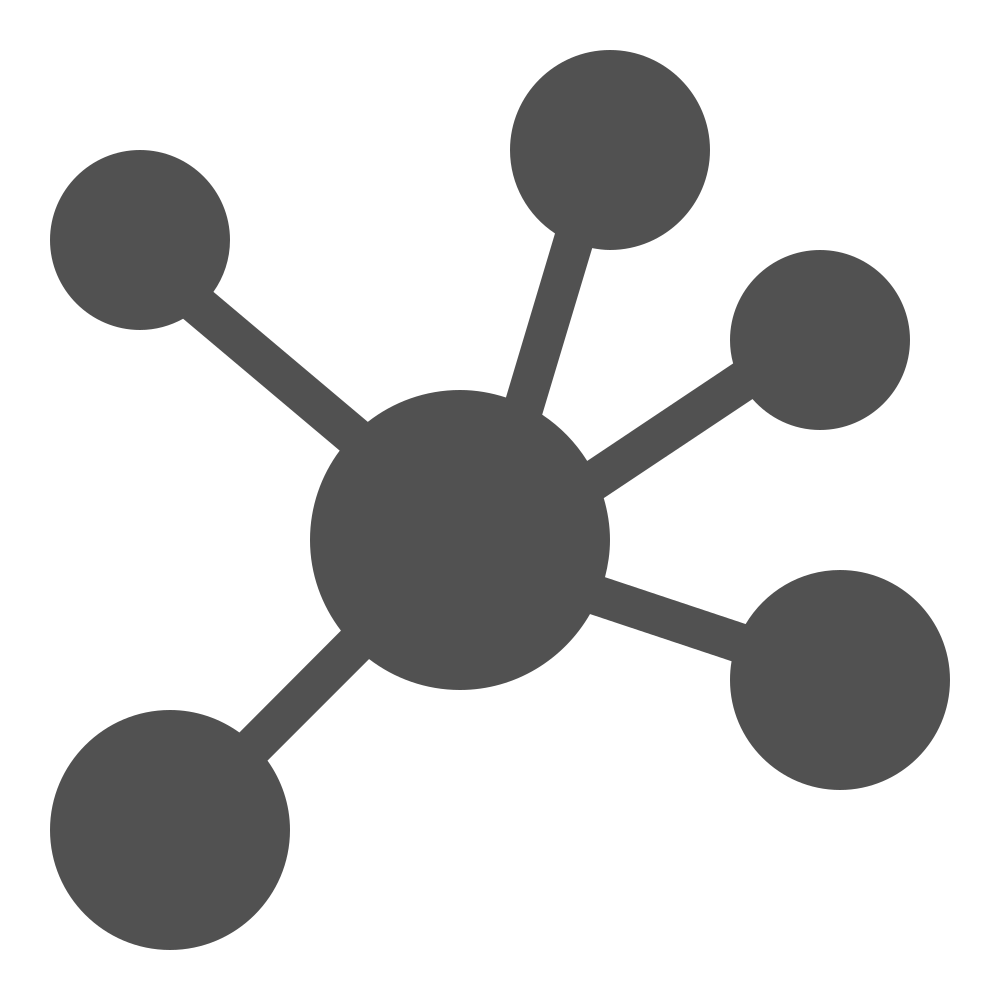
\includegraphics[width=0.5\textwidth]{membrane-logo}\par\vspace{1cm}
	{\huge\bfseries Membrane\par A Peer-To-Peer File Backup System\par}
	\vspace{1cm}
	Submitted by 
	{\Large\itshape Dominic Hauton\par}
	
	
	\vfill
	
	
	\justifying
	\noindent
	\textbf{COPYRIGHT}
	
	\vspace{0.25cm}
	\noindent
	Attention is drawn to the fact that copyright of this dissertation rests with its author. The Intellectual Property Rights of the products produced as part of the project belong to the author unless otherwise specified below, in accordance with the University of Bath’s policy on intellectual property (see http://www.bath.ac.uk/ordinances/22.pdf).
	
	\vspace{0.5cm}
	\noindent
	This copy of the dissertation has been supplied on condition that anyone who consults it is understood to recognise that its copyright rests with its author and that no quotation from the dissertation and no information derived from it may be published without the prior written consent of the author.
	
	\vspace{0.5cm}
	\noindent
	\textbf{DECLARATION}
	
	\vspace{0.25cm}
	\noindent
	This dissertation is submitted to the University of Bath in accordance with the requirements of the degree of Bachelor of Science in the Department of Computer Science. No portion of the work in this dissertation has been submitted in support of an application for any other degree or qualification of this or any other university or institution of learning. Except where specifically acknowledged, it is the work of the author.
	
	\vspace{0.25cm}
	\noindent
	\emph{Dominic Hauton}
	
\end{titlepage}

\renewcommand{\abstractname}{Abstract}
\begin{abstract}
Membrane is an amalgam of distributed storage and backup software, designed to operate on a very large scale: terabytes of data backed up across thousands of users across the world. A Membrane user is able to trade storage space with peers across the network, allowing them to securely store their backups world wide providing the user with data resilience with high availability at no monetary cost to the peer.

The applications vary from users who require a secure backup tool with file versioning for their important documents, to corporations that need to provide data resilience to their employees without investing in infrastructure, instead making use of redundant storage space on employee terminals.

In this report we follow the design and construction of Membrane, drawing on knowledge from distributed storage, intelligent agent technology and existing backup tools, finishing by providing a sound analysis of the completed solution. The software created succeeds in all test scenarios providing an easy install that requires no domain knowledge, capable of reconstructing backed up files directly from the peer swarm. 
\end{abstract}

\tableofcontents

\renewcommand{\abstractname}{Acknowledgements}
\begin{abstract}
\vspace{2cm}
I would first like to thank my project supervisor Dr.~Russell Bradford, who has provided excellent advice and guidance throughout the year.

\vspace{0.75cm}

To my parents for providing me with unfailing support and continuous encouragement throughout my years of study. This accomplishment would not have been possible without them.

\vspace{0.75cm}

To Tom and Jason, who have given me great joy and support throughout my four years of University, helping shape both my life and work.

\vspace{0.75cm}

To the developers of the open-source libraries used throughout development. Without their work the created software would not be possible.

\vspace{0.75cm}

Finally to my other family members and friends who have supported me along the way.

\vspace{0.75cm}

Thank you.

\end{abstract}

\listoffigures

\chapter{Introduction}
Distributed storage is a well studied and explored domain with clear advantages over storage on a single machine. In this project we analyse, design and build a amalgam of distributed storage and backup technology. We must first decompose the problem into several parts and explore advances made in fields such as cryptography, file backup and intelligent agents as well as looking at advantages of existing technologies.

Throughout the remainder of the introduction we discuss the goals of the project and justify the creation of Membrane, analysing existing solutions and describing challenges we may face.

\section{Project Goals}

Membrane allows users to easily backup and recover the contents of folders on their computer without needing to pay for a subscription-based service. Looking at a breadth of products available it quickly becomes evident that there is a huge desire for external backup, and cloud storage services such as Dropbox and Google Drive have become a household name. \citep{dropbox2015popularity}

To compete with existing solutions we aim for two important features: 

\begin{itemize}
 \item A simple installation
 \item The ability to backup files and recover them from peers after data loss.
\end{itemize}

On a centralised backup system this a trivial task, however, with a distributed system the concept of creating an account, logging in, finding peers and discovering which users hold your files is a much greater challenge requiring users to create unique credentials that will be recognised throughout the swarm locally and technology from distributed systems like BitTorrent to track down files.

In this project we are working towards a proof-of-concept, creating the fundamentals of the Membrane and focusing on the key aspects of distributed backup. We exclude features that are simply a convenience to users, leaving them for later development if the project proves successful.

We follow the minimum feature set methodology described by \cite{blank2010mfs}, a practise which is now used heavily amongst technology startups. The technique aims to focus on defining features of applications, reducing engineering time to receive feedback from users as early as possible, shaping further development.

The first step of the project will involve looking at existing products, seeing what design lessons from them we can apply to Membrane. We will then approach potential users and inquire what features they think are important in the system. A technology survey will be performed to assess what technologies we can use to ease development and create a set of requirements. The solution will be built and tested taking back user feedback and using this in our final verdict.

\section{Need for Membrane}

With the advent of cheap high-speed internet people are able to use cloud services to backup data. These tend to be expensive for anything but small amounts of storage and many people have expressed security concerns over holding their data in a data centre owned by another company. \citep{batters2010dbsecurity} Especially if their data leaves the users country where data protection laws may be different.

Over time personal storage capacities for users have also increased. It is now common for computers to come with large amounts of hard drive space which is often not filled to capacity. The project proposed promises to swap this free hard drive space to back up other users’ data in exchange for their surplus space to backup your data.

To simplify the process, the system will be able to negotiate contracts of varying complexity for space allocation on another machine, in exchange for space on itself. Unlike most distributed databases and cloud storage solutions, frequent down-time will be expected across devices and contracts will have to account for this.

There is an open gap in the market for a distributed storage solution which focuses entirely on backup and trading data, rather than charging a fee for storing data. The users of Membrane would be able to benefit from the advantages of commercial services, without the associated cost and security concerns.

The applications of distributed backup vary. Three examples include home users who require a secure backup tool for their important documents, that ensures their data will never be analysed by the person storing them. Groups of friends that want to store family photos with each other, thereby spreading their data across multiple locations and protecting them from tragic events like house fires. Corporations that need to provide data resilience to their employees without investing in infrastructure, instead making use of redundant storage space on employee terminals.

\section{Challenges}
There are multiple challenges associated with creating both decentralised systems and backup solutions.

Distributed storage systems rely on sending data back and forth between users, typically using large amounts of bandwidth in the process. In addition, to prove to peers that their data is still being held, calculations need to be performed on the data using both the disk and processor. It is important that the user's work is not interrupted by Membrane, so steps will need to be taken to keep resource usage down to a minimum.

A method for minimising backed up data is required to be able to store as much data as possible. An effective method of managing where file chunks are stored, a mechanism to encrypt the files on the remote peer and a way to periodically verify that the peer still holds the file.

Part of the required research also includes exploring trust metrics, a field closely related to Intelligent Agents. We look towards the advances there to make storage decisions based on the trust and reputation of other peers in the network using known previous behaviour.

\section{Modules}

Membrane will be built up of several predetermined modules performing distinct roles. These have been broadly identified at this stage as a guide for our literature review and for technology decisions.

The core of any backup system is the file system watcher that determines whether a file has been modified, added or removed. This must be able to cheaply assess if a file or folder has changed and determine whether the altered file needs to to be updated in the storage system.

Once a modified file has been detected that change needs to be catalogued and the bits required to restore the file must be stored locally for further processing. This causes temporary duplication, however this must be performed so modification to the real files can continue while a peer willing to store the file is located. This system must also be able to recreate the file from the bits stored.

Next a system needs to be put in place to package bits from various files into a block of data that a peer can store. This system needs to be able to determine which peer certain bits should be stored with and how many should store the file, based on trust, availability and other useful metrics that will be explored.

Finally a module responsible for networking and authentication must be created. This must be able to authenticate the user, find peers, establish connections to new peers and deal with the challenges to creating a secure communication link to the peers.

\section{Planning}

We use four techniques to ensure the project stays on track from start to completion.

\begin{itemize}
 \item Scrum Board
 \item Gantt Chart
 \item Weekly Supervisor Meetings
 \item Weekly Goals
\end{itemize}

A scrum board is a planning technique taken from software development. Tasks are split into three categories: to-do, in-progress and complete. The system revolves around adding tasks to the to-do section of the board clearly displaying everything that needs to be done, giving us the ability to easily determine what the next task should be.

A Gantt chart is used for long term planning. We divide the project up into its constituent parts: proposal, literature review, development and dissertation. From there we can easily decide what parts of the project impact what other parts to develop an overarching strategy for completion. It also provides a convenient way to see when progress is ahead of, or behind projections.

Weekly supervisor meetings keep the project on track throughout and help decide what steps need to be taken next, particularly if unexpected events occur and the project needs to be altered to compensate.

Finally we used weekly goals to ensure a good amount of work was done consistently throughout the project. An example of a weekly goal might be ``Two peers are able to connect''. This goal can then be dissected into tasks and placed on the Scrum board.

We have included an example of the Gantt chart from February, five months into development in figure \ref{fig:gantt}.

\section{Summary}

Cloud backup solutions are expensive and do not offer much security when storing user's data. Membrane aims to challenge this limitation by providing a free and secure backup service that uses a network of peers to store data.

We expect challenges with resource utilisation, account creation and a method to select peers for backup and verifying they are still holding the data. We have also discussed the basic structure of Membrane describing the overall planned functionality for individual modules. We will explore these further in our literature review.

\chapter{Literature Review}

The literature review aims to preempt challenges by finding solutions to similar problems in literature and existing pieces of software.

We will first explore the history of file backup, proceeding into the challenge of locating, trusting, connecting and communicating with peers. Finally we will look at authentication issues as well as exploring how a peer can prove they own a file, without re-sending the entire file back to us.

\section{History of Problem}

A file backup can be trivialised to simply copying a file to another location. In order to keep the backup up-to-date the current file and the backup must be compared. The program \code{diff} solves this through finding the longest common sub-sequence of bytes between files. In order to improve performance: hashing, presorting into equivalence classes, merging by binary search, and dynamic storage allocation are used. \citep{hunt1976algorithm}. This allows the user to view changes and copy the file over again if required.

\subsection{Rsync}
In a networked scenario, bandwidth from source to destination is at a premium. Rsync, introduced in 1996 presents a much better solution through copying changed file chunks (deltas). \citep{tridgell1996rsync} It splits the file into shards\footnote{Sections of the data.} and calculates a weak rolling checksum and strong MD4 checksum for each shard which allows quick comparisons of shards along the file. When a discrepancy is found, we assume an extra byte or bytes have been added to the file. The weak checksum can be efficiency recalculated for the next offset and once there is a match, it is confirmed with the strong checksum. The new added chunk can now be transmitted. This results in a lot less data being copied than there would be with a diff file. \citep{tridgell1996rsync} This combination of weak and strong check-sums has been used across multiple distributed systems including low-bandwidth file systems \citep{muthitacharoen2001low} and high performance transactional object stores. \citep{stephen2000platypus}.

Multiround Rsync improves on the rsync algorithm by allowing for more communication to lower bandwidth. Shards of smaller and smaller sizes are used to find holes in the old file, each round looking at more and more specific bits in the files until the minimum shard size is reached and a copy occurs. \citep{multiroundrsync} This works better than standard rsync in situations where the source file has been changed in many places distributed around the file.

Rsync requires both old and new copies of a file to exist on the host system during an update. This issue has been addressed by creating an in-place rsync (ip-rsync) that uses techniques compression techniques to move the areas of the file around. In ip-rsync file sender sends add and move commands to the destination in an order that guarantees no files will be overwritten. \citep{rasch2003place}

\subsection{Git}

Git is an improvement on Rsync in terms of file backup as it provides both version history and minimises data transfer. To keep storage simple, a copy of the whole file is stored and a reference is put into the version history. By storing old files locally operations are fast and the system can operate without a centralised server. To reduce file duplication all files are referenced using their SHA-1 hash. This means you can be sure the contents of the file hasn’t changed since you last read it. \citep{torvalds2010git}

Git also uses a 3 stage workflow. A working directory, where the current files are stored, a staging area and a .git directory. The staging area prepares your next commit\footnote{A snapshot of current state of the files.} and then it is finally committed. When the staging is complete the change is irreversibly stored. This is a good approach that will be adopted in the final software solution. It will allow incrementally finding changed files, and assessing the need for a new version number to be saved.

\subsection{Bittorrent}

The BitTorrent protocol is a mechanism for sharing files between swarms of hosts. BitTorrent splits files into parts and can transfer them out of order, so peers start sharing data even before they have received the full file. Each file has a SHA-1 identifier, similar to Git. \citep{qiu2004modeling}

If a user wishes to download a file from the swarm, the user downloads a metadata file from the web and locates users sharing the data using a Tracker Server, Distributed Hash Table (DHT) described in section \ref{sec:shard-discovery} or Peer Exchange (PEX). \citep{cohen2008bittorrent}

A Tracker server is a centralised store of all current connected users along with how much of the file they hold. This approach is vulnerable to exploitation by authorities as all of the data about a swarm is stored on a single server. Ideally we want to be able to avoid this in the final implementation of Membrane to prevent any one server holding a large part of the information about the swarm.

PEX described in section \ref{sec:pex} is a method for two clients to share a subset of their peer lists. Coupled with DHT, PEX removes a vulnerability from the BitTorrent network by allowing fully distributed bootstrapping, tracking and peer discovery.

\subsection{Resilio}

Resilio Sync is an example of a distributed file storage system that utilises the BitTorrent protocol to automatically synchronise folders between a user’s systems. It is not a cloud backup solution and not intended as a form of off-site storage. There is no distributed file system and as a result, no redundant data block algorithm adding complexity. \citep{farina2014bittorrent}

As Resilio Sync uses DHT to transfer data, there is no central authority to manage authentication or log data access attempts. This makes it difficult to determine whether a file has been accessed by another user. \citep{farina2014bittorrent} The assumption has to be made that everyone in the network has access to all encrypted file chunks. To access and reassemble a file, a user will be required to request all of the file chunks individually and then locally reassemble them.

\subsection{Storj}

Storj is a peer-to-peer cloud storage network which aims to allow users to store files on a decentralised platform. The platform takes special care to provide protection against Sybil\footnote{Identity forging.} attacks and other forms of fraud. \citep{Wilkinson14storja}. To store files it stores encrypted hashed shards on the network. In order to provide proof-of-storage it uses Merkle Audits and pregenerated audits with hash-challenges to determine whether the client still holds the required data. By adding a seed to the hash-calculation the client can enforce the workers are still in possession of the data. It prevents the client cheating a farmer through using blockchain proof-of-existence to keep both parties honest.

The most efficient form for proof of storage found in Storj is through using a deterministic heartbeat. Using Feistel permutations data can be verified with $n + 2 \sqrt{n}$ challenges. This is less I/O intensive than a full heartbeat which checks all of the file, but still allows an attacker to complete heartbeats with only a data integrity of $\frac{1}{n}$, where n is the number of nodes holding the data.

In order to add extra protection to files, we could use erasure coding\footnote{A method of redundancy in which a file is split into shards, and the shards are expanded with redundant data pieces to allow for the loss of one or more shards without encountering data loss.} to allow file recovery if one of our shard types is lost. This can be investigated in our software, however, as shards are expected to change on a regular basis because of versioning, this may not be possible.

To prevent Sybil based attacks, Storj encrypts each shard segment with a different salt\footnote{A random bit of data.}. This stops workers completing proof-of-storage on behalf of another node.

\section{Peer Admission}

The first step in designing the distributed backup system is locating other peers within the swarm. This is accomplished through Peer Admission. Once the first peer is found data within the swarm could be located using a DHT which guarantees content can always be found.

\subsection{Bootstrapping}

There are two types of P2P networks which must be examined:

\begin{itemize}
 \item \emph{Asynchronous}
 \item \emph{Synchronous}
\end{itemize}

Within Synchronous networks the number of nodes on the network is constant and all of the nodes are aware of each others existence. This does not allow storage networks to scale but it does allow data to be kept private. \citep{saxena2003admission} This is the simplest and first approach that will be investigated in locating nodes within Membrane.

In most current P2P systems such as Gnutella \citep{klingberg2002gnutella}, Chord and Tapestry as well cryptocurrencies\footnote{Bitcoin and Litecoin} a bootstrapping node is contacted to provide information about what clients are currently online. Once a bootstrapping node allows the client to find the edge of the swarm, more information can be found using peer exchange.

Within a local network we can also use Universal Plug and Play to find other nodes within the local network. This prevents an external call to a bootstrapping node and as a result is less prone to snooping.

Through looking at availability metrics within BitTorrent systems \cite{neglia2007availability} determined that both trackers and DHT should be used in creating a highly available distributed storage system such as BitTorrent. DHT tends to be slower at finding new data, however it is much more reliable.

Within Membrane, we plan to use a combination of asynchronous and synchronous techniques. Peers try to bootstrap from their last known neighbour nodes on the network taking advantage of the fact that IP addresses change fairly infrequently. It would be unlikely that all peers have changed address. If this fails, the system can contact a bootstrapping node. Ideally this should only happen during a first install. Throughout the lifetime of the application the centralised bootstrapping node would ideally be used less and less by peers.

Users could potentially also be allowed to provide a host name if they have set up Dynamic DNS (DDNS) \citep{bound1997dynamic}. This would completely remove the need for a bootstrapping server.

\subsection{Peer Exchange} \label{sec:pex}

When bootstrapping is complete peers can increase their knowledge of the network through Peer Exchange. This is used by BitTorrent to help share swarm information with other nodes. As soon as a client connects to the swarm, peer information is collected using DHT or PEX.

There are two common extension protocols which send at most one message a minute when a client leaves or exits the swarm. To reduce congestion at most 50 peers can be added or removed in one PEX message. \citep{vuze2010vuze}

We look into this as our primary way for discovering new peers.

\subsection{Shard Discovery} \label{sec:shard-discovery}

BitTorrent also uses the Mainline DHT to find other hosts in the network. This is a Kademlia DHT which according to \cite{jones2015mainlinedht}, now supports 25M users. It works through assigning each node and file a 160-bit string as an ID. We can work out which node is meant to store a file metadata and crawl in the direction of the node using a hill climb algorithm. Once shard location is stored on the appropriate host in the DHT, the shard can be rediscovered by any node on the network.

Hosts in Membrane could potentially store an encrypted metadata file with all local mappings for which host owns which shard and which IP belongs to each host. A DHT could serve as a mechanism for recovering from total data loss.

\subsection{Dynamic IP Address}

Dynamic IP addresses have proven to be problematic in distributed computing. Internet Service Providers (ISPs) typically charge more for users to have a static, unchanging IP which few users opt for.

BitTorrent tackles this issue through using a DHT to dynamically find the IP address of the user that owns a shard. This approach is robust, however, it is a complex solution to IP address resolution to which simpler and easier to implement methods may be available.

Another widely used approach is using Dynamic DNS (DynDNS) as described by \cite{bound1997dynamic} in RFC 2136. This allows a client to automatically update a nameserver with new IP information, allowing clients to have a persistent addressing method for devices that change their IP frequently. This approach requires initial configuration by the user, however, it provides a reliable way to connect with a user when their IP is lost.

There are several tools such as MintDNS, cURL and Iandyn that could be used to ease the development of a built in DynDNS. When setting up a relationship with another host, both an A/AAAA Address and CNAME could be provided, where the CNAME is a backup if the A/AAAA address does not work.

To resolve IP Address resolution within Membrane, we would like to propose a new method of discovering users that takes advantage of small-world networks. \citep{porter2012small}

In small-world networks, the mean shortest-path between two nodes increases slowly compared to the number of notes in a network. Within a group of users in Membrane hosts are likely to share multiple first, second and third degree connections. By storing a list of IP addresses from all of the hosts we simply try to connect to all hosts were previously connected to. It is highly unlikely that all connections will have changed IP address and we can then rebuild our know IP address list.

We take inspiration from ARP \citep{plummer1982ethernet}, and send broadcasts to the network to see if anyone is aware of the current address of a host. The downside of this approach is that it relies on the node within your social network to be online. Measures will need to be put in place to reduce broadcast spam.

If we choose to forward these broadcasts we need to be weary of broadcast storms, runaway broadcast events common in networks that used broadcasting for communication. \citep{Tseng:2002:BSP:506900.506905} These can be mitigated by reducing broadcast traffic. The first step to limiting these potential broadcasts, is implementing a hop count on broadcasts. This is commonly seen in routing protocols such as IPv6 \citep{deering1998internet}. The Spanning Tree Protocol (STP) as seen in IEEE 802.1d \citep*{ieee802ieee, sharma2004viking} provides loop-free routing in LANs by pruning redundant links. Topology changes are dealt with by rebuilding the tree.

Within Membrane rebuilding a Spanning Tree would be an expensive operation. If broadcasts become a problem a 'block request' system can be used, similar to that of ICMP redirects. \citep{postel1981rfc} If a node receives a duplicate broadcast message it sends a request back one hop, asking the peer to not send broadcasts from that source toward it for  some time. The time limit would allow for corrections if the network topology changes. This preventative approach and could be improved by using the full Spanning Tree implementation and further enhanced by using a DHT closest jump approach if required.

\section{Data Allocation on External Nodes}

In order to store data on another node Membrane must first have permission to store files on another node. To decide which peer to request this permission from, we must be able to look at trust information for peers on the network, and negotiate and trade space once a suitable candidate has been found. These two areas have been explored in the context of Multi Agent Systems (MAS) in the past. \citep{wooldridge2009introduction}

\subsection{Negotiation} \label{sec:neg}

Negotiation aims to reach a level of resource allocation that is acceptable for all involved parties. \citep{rahwan2005interest} It allows two or more parties that value each others service, to participate in a mutually beneficial exchange of services, however, as there are multiple beneficial outcomes it can be defined as ``distributed search through a potential space of agreements'' \citep{jennings2001automated} Within Membrane, this service is storage space, that is physically separated from the current user. We now take a look at negotiation and how we can build a negotiation framework that our agents can use to exchange storage.

There are three main areas that are important for negotiation. Negotiation protocols, negotiation objects and the node's reasoning models. \citep{beer1999negotiation} The sophistication of the negotiation is determined by each of these and can take different forms such as auctions, argumentation and protocols in the style of a contract net. The simplest negotiation uses fixed size items. These could be further augmented by counter offers and stronger guarantees in more complex negotiation systems.

A simple negotiation protocol issues a call for proposals to a number of nodes and waits for their bids. To formalise this a Agent Communication Language (ACL) such as the Knowledge Query and Manipulation Language (KQML) \citep{finin1992specification} or the more modern Foundation for Intelligent Physical Agents (FIPA) \citep{fipa2002fipa} is used.

\citep{rahwan2005interest} \cite{beer1999negotiation} tells us that within KQML the agent sending the query is expected to decide how the receiver will handle it, which places limits on negotiation. On the other hand, FIPA is newer and as a result could be more error prone.

\subsection{Negotiation Logic}

The form of negotiation within Membrane also needs to be decided. We must first decide on a reasoning mechanism to use within the agent. The distinction between monotonic and non-monotonic logic is important in the study of AI and multi-agent systems (MAS). In non-monotonic logic new axioms (or knowledge) can invalidate old theorems. \citep*{mcdermott1980non, antonelli2008non} This is important in the real world as we need to be able to make assumptions on facts and retain flexibility in our understanding of the world.

Within a MAS a non-monotonic logic can be more difficult to implement as theorems need to be constantly asserted, and as a result they often resort to first-order (or monotonic) logic. Within Membrane we need to implement a monotonic logic to calculate trust in our contracts and negotiations. In the context of a negotiated contract, throughout its duration, we cannot afford to re-evaluate our trust of the agent.

\subsection{Negotiation Tactics}

In order to exchange storage space we must find the most suitable node in the network. There are multiple negotiation tactics between agents for collaboration and coming to an agreement. \citep{beer1999negotiation} We shall explore the advantages and disadvantages of game-theoretic approaches \citep*{rosenschein1994rules, kraus2001strategic, sandholm2002algorithm}, heuristic-based approaches \citep*{faratin2000automated, fatima2002multi} and argumentation-based approaches \citep*{kraus1998reaching, jennings1998argumentation} as well as exploring practical implementations negotiation.

Ideally a negotiation mechanism is computationally cheap, produces good outcomes, distributed, fair to all participants, compatible with fixed strategies and is able to function without complete information. \citep{rahwan2005interest}

Using a \emph{game theory} approach we assume all agents are self-interested and allows agents to analyse optimal behaviour. \citep{osborne1994course} We can apply this in agent reasoning by giving each combination of collaborations a utility. Doing this an optimal set of interactions can be calculated. This can even be used to help agents interact in a certain way. \citep{varian1995economic}. The main downsides include the assumption of unbounded computational resources, complete knowledge of the outcome space. \citep{rahwan2005interest} This makes a game theory approach difficult to use in Membrane as information about the entire network is not known.

A \emph{heuristic} approach produces 'good enough' negotiations. Instead of exploring the full extent of possibilities they focus on the subset most likely to lead to positive interactions. In the context of Membrane, this may be hosts that you have had successful interactions with before. The downsides of this approach is that it becomes difficult to predict the negotiation actions of other agents and as the full search space is not explored the result may not be optimal. \citep{jennings2001automated}

A \emph{argumentation} approach is beneficial when a flexible negotiation is required and the agents have limited knowledge of the world. It is commonly used in the human world by advertisers to convince consumers to try products. \citep{slade2002reasons}. Instead of simply rejecting an offer a agent can say why or offer a counter-proposal, which can result in more successful negotiations.

Although this approach offers far better negotiation, it is much more complex to implement and is not required within initial implementations of Membrane. In the future when we look towards more complex contracts with different requirements, we may require this to help find a peer offering a service we desire.

\subsection{Practical Negotiation}

We now look at practical real-world negotiation. Real world approaches take into consideration the practical implications of reasoning systems and often use more pragmatic approaches with that concepts work.

Within cloud computing an agent is often required to request a service. The use of these resources is based on service-level agreements (SLAs) which are designed to provide users with a service when requested. \citep{paletta2009mas} One critical issue in SLAs determining the Quality of Service (QoS) constraints of the offered service.

\cite{yan2007autonomous} explores creating a SLA negotiation system, splitting SLA negotiation into three parts. Defining \emph{Negotiation Protocol} that allows participants to send offers to each other, \emph{Negotiation Coordination} which ensures the final result of the negotiation fulfils the QoS requirements of the agent and a \emph{Decision Making Model} which allows the parties to decide if they are satisfied with the deal.

Within Membrane, hosts are unable to know if they will be compatible with another agent. It might be the case that they both have 50\% uptime, however they are never online at the same time. As a result a system will have to be created to allow agents to find if they are compatible with each other and storage decisions will have to be based on this.

\cite{paletta2009mas} presents an negotiation mechanism that uses key awareness concepts first proposed by \cite{herrero2007agents}. It uses an quantitative metric in the range [0, 1] to decide how much the agent should be collaborating with another agent. The agents can then communicate using the messages:

\begin{enumerate}
 \item REQUEST - Can you perform A?
 \item CONFIRM - Yes I will do A.
 \item DISCONFIRM - No I will not do A.
\end{enumerate}

Collaboration decisions are decided using an Artificial Neural Network (ANN). Three metrics are used, physical resource availability, if the node is available for collaboration and the number of previous collaborations of the same type. The ANN used was a Multi-Layer Perceptrons (MLPs) using one hidden layer and two units.

When evaluated the mechanism was able to deal with 93\% of situations and negotiation with the first node was successful 68\% of times. \citep{herrero2007agents}

Within Membrane we will aim to produce a new negotiation mechanism built into the  contract system similar to \cite{paletta2009mas}s. We aim to use a feedback loop, where good behaviour results in upgraded contracts, that in turn result in increased good behaviour. This is discussed further in section \ref{sec:contractMech}. We hope this a fair and cheap method of matching peers as required by \cite{rahwan2005interest}.

\subsection{Service Level Agreements}

In order to create a negotiation system we need to explore what makes up an successful software SLA. \cite{keller2002defining} defines the WSLA framework which sets out to create a SLA based negotiation frame work.
They describes 3 key areas that must be present in an SLA.
\begin{enumerate}
 \item Parties Involved
 \item Service Description
 \item Obligation
\end{enumerate}

Within Membrane the parties involved will always be the two nodes exchanging information. The service description will be a promise to store a block of data on another host. The obligation will include various parts such as proof-of-storage and the ability to update and retrieve the data a set number of times. These will be explored when the SLAs for membrane is designed.

Another key area \cite{keller2002defining} discusses is the 5 stages of an SLA life-cycle.

\begin{enumerate}
 \item SLA Negotiation and Establishment
 \item SLA Deployment
 \item Measurement and Reporting
 \item Corrective Management Actions (in case of violation)
 \item SLA Termination (in case of violation)
\end{enumerate}

These are the backbone of every real SLA and will be explored in more detail while designing the negotiation system for Membrane.

\section{Trust and Reputation}

Agents in a distributed system need to be able to protect themselves from `bad' peers. \cite{pinyol2013computational} describes three main approaches to control the acts of agents. The \emph{security approach} which guarantees the authenticity and integrity of interactions. The \emph{institutional approach} which relies on a central authority to enforce good behaviour and finally the \emph{social approach} which allows agents themselves to punish other agent for 'bad' behaviour. This final approach is where trust and reputation is used.

Trust can be used to predict the behaviour of an agent. \citep{wooldridge2009introduction} A classification presented by \cite{balke2009using} defines 5 stages that exist in reputation and trust models. Co-operative behaviour is first stored and then rated using a utility function.

Within Membrane it is easy to see the utility being rated as shared uptime. This cooperative behaviour could then be stored in an image of the peer at a predetermined level of detail and recalled to infer trust. Finally the agent can use this trust to learn and adapt its strategy.

The ReGreT model \citep{sabater2001regret} is ``one of the most complete reputation and trust models'' \citep{pinyol2013computational} so we use it to see what a good trust system includes.

It uses direct experience, third party information and social structures to calculate trust, reputation and credibility of another agent. An important note for this model is that trust is contextual. Agent A will trust B while certain conditions are met. In the context of Membrane, perhaps another agent will refuse to return our data, if we cannot prove that we still have their data, which would mean that they would be useless if the client experienced completed data loss. We must therefore consider periodically simulating a situation in which complete data loss was experienced to ensure the backup system will work when required.

\subsection{Trust and Reputation Attacks} \label{sec:tar}

Attempts to misrepresent reliability and manipulate reputation are common in traditional communities and have been exploited by con artists for centuries. In a distributed system agents must be able to protect themselves against common trust attacks. \cite{josang2009challenges} describes 9 potential attacks on reputation systems.

\begin{itemize}
 \item Playbooks - Gain high reputation and burn it quickly with low quality actions
 \item Unfair ratings - Give incorrect reputation or image
 \item Discrimination - Give high quality service to one set of users and low quality to another set
 \item Collusion - A coordinated reputation attack.
 \item Proliferation - Offer a service through multiple channels
 \item Reputation Lag Exploitation - Provide a large number of low-quality services quickly
 \item Reentry - Change identity to recover reputation
 \item Value Imbalance Exploitation - Gain reputation with easy actions
 \item Sybil Attack - Inflate reputation with fake accounts.
\end{itemize}

When implementing a trust system in Membrane these attacks should be considered and special attention should be paid to prevent a new user being exploited for their storage space when joining the swarm.

\section{Communication} \label{sec:comm}

As Membrane is a distributed system, communication is key for nodes on the network to interact. It is traditional to form a protocol that agents can use to share information with each other. These protocols are often very rigid and do not allow for expansion.

We look to ACLs which provide a formal but more flexible approach that aims to let agents share a common understanding of the domain, and allows hosts to reason about communication themselves.

\subsection{Agent Communication Language}

FIPA is an ACL based on Speech Act Theory \citep{labrou1999agent}. It splits communication into a communicative act (CA), an ACL message structure and a set of communication protocols such as XML or OWL (Web Ontology Language). In FIPA communication should be rational, in that when sending a message:

\begin{itemize}
  \item The sender believes the proposition.
  \item The recipient does not already believe the proposition.
  \item The recipient will begin to believe the proposition after it is made.
\end{itemize}

In the case of Membrane this could be put into the context of asking another node to store data, it would only be reasonable to send another node data to be stored, if the two nodes had negotiated storage of that block between them previously.

To keep communication simple for nodes, we shall use two CAs

\begin{itemize}
  \item REQUEST
  \item INFORM
\end{itemize}

where \emph{REQUEST} expects a reply of some sort and \emph{INFORM} does not. This will enable easier implementation and can be expanded if required.

\subsection{Ontology} \label{sec:ontology}

An ontology is a way of defining basic terms and relations comprising the vocabulary of a topic area. \cite{sugumaran2002ontologies} tells us the the three most commonly used relationships in an ontology are \emph{is-a}, \emph{synonym} and \emph{related-to}\footnote{A generic association between entities}. 

\cite{noy2001ontology} lists the benefits of ontology within distributed systems:

\begin{itemize}
 \item Enable common understanding of the structure of information
 \item Enable reuse of domain knowledge
 \item Make domain assumptions explicit
 \item Separate domain and operational knowledge
 \item Analyse domain knowledge
\end{itemize}

Within Membrane we may benefit from an ontology during negotiation for storage space. Obligations could be predefined between agents and an agent could request a set of obligations, instead of explaining an obligation during negotiation. This allows agents to be more concise and expressive.

\section{Peer-to-Peer Connection} \label{sec:p2pconn}

Network Address Translation (NAT), defined in RFC 2663 by \cite{srisuresh1999ip} is used extensively to solve the IP exhaustion problem by mapping an internal network IP address to an external IP. It unfortunately creates a lot of well documented problems for peer-to-peer communication where a host's internal IP is only valid on the same private network. If multiple hosts are behind the same NAT gateway they all have the same external IP address.

In order to contact a peer behind a NAT gateway the gateway needs to know which peer we wish to contact, done by using a specific internal port that the gateway has mapped to that peer. There are four major NAT-Traversal techniques described by \cite{ford2005peer} that allow us to achieve this.

\emph{Relaying} is a method of communicating through a well known server, that has a static IP address and port. This has the advantage of being simple, however, it has the disadvantage of using the server's processing power, network bandwidth and increases latency between peers. It is a good fallback strategy but also requires both clients to initiate the connection, which makes listening for incoming connections difficult. The TURN protocol \citep{rosenberg2005traversal} describes a fairly secure method for relaying.

\emph{Connection Reversal} is the use of an external server to request a `call back' to a host. The connecting host contacts an external server with a target host and leaves it's public IP and port. The relaying host can then choose to send a request to host behind NAT and the host behind NAT can choose to forward the request. It has similar limitations to relaying, however, it is easy to imagine an implementation that uses connection reversal for bootstrapping a P2P connection.

\emph{UDP Hole Punching} is a technique defined in RFC 3027 5.1 \citep{holdrege2001rfc} that allows two clients behind NAT to connect with the use of a rendezvous (RV) server. Hosts contact the RV and leave their UDP port and address. We need to be weary of poor NAT implementations translating IP addresses within data when packets are coming in and out. \citep{ford2005peer}

The initial outbound packet from a host to a the RV server is key in `punching a hole' through the NAT. The timeout of a hole punched port can be as low as 20 seconds, so the host must maintain the hole by sending single packets to the RV on a regular basis.

\emph{TCP Hole Punching} is more complex than with UDP as clients need to establish sessions across the NAT. For hole punching to work the same port needs to be used for listening and establishing a connection and a new port needs to used for handling the connection.

Hairpin NAT allows for two clients behind the same NAT gateway to connect to each other without any address translation avoiding overheads. We must consider the possibility that the gateway has this incorrectly configured if performance issues arise.

UPnP \citep{boucadair2013universal} is a method through which a host can request a NAT gateways to open a port for the application. There have been security concerns with UPnP which has resulted in UPnP being disabled on many routers.

It's important to consider that the ports behind a NAT are dynamically allocated, so connections must be authenticated between connections, to ensure the IP address and port still direct towards the same host.

There are two practical solutions that I shall explore for implementation within Membrane. TURN \citep{wing2010traversal} which provides a set of methods for TCP hole punching and a combination of UPnP and relaying. Membrane can ask the router to open up a port and then send the information of that port to the RV server.

\section{Distributed File Systems}

Membrane shards files and stores copies on multiple nodes for redundancy. This is a technique that is commonly found in distributed file systems (DFS) such as Hadoop File System (HDFS) \citep{hdfsAnalysis}, Google File System (GFS) \citep{TheGFS} and Parallel Virtual File System (PVFS) \citep{ross2000pvfs}. This section aims to explore the reasoning and decisions taken with these file systems.

HDFS has proved to be highly successful in storing large quantities of data over thousands of nodes and is used by over 100 organisations world wide. Both HDFS and GFS \citep{mckusick2010gfs} store file system metadata on a central dedicated server called a NameNode \citep{hdfsAnalysis}. Ceph takes this approach further, storing file meta on a distributed cluster of NameNodes, using hash function to spread metadata over the name nodes. \citep{weil2006ceph}

The NameNode stores the metadata as a combination of a checkpoint and journal (a write-ahead commit log). If there is a fault on the NameNode, such as a power outage, the journal can be replayed over the latest checkpoint and a new snapshot is created during a node restart.

In HDFS, during startup a DataNode connects to a NameNode, and performs a handshake with a unique storage ID that can identify it. In addition a DataNode will also send heartbeats and reports on a regular basis. \cite{hdfsAnalysis} This is a great approach as it makes the DataNode responsible for notifying the NameNode that it still holds the data. Not the other way around. 

In both GFS and HDFS data is streamed directly from the client to the DataNode in 64k chunks and a checksum is sent with the original file to assert the transfer was successful. Both systems also have a default of 3 replicas per shard. TCP is used for communication as it provides reliability and a session for transfers. Chunks are given a 64bit chunk handle.

Membrane takes the approach of a NameNode storing file metadata on the user's system and then redistributing it with the data. The metadata will include checksums for shards, modification dates, encryption type and compression type for each shard, as well of the list of files the shard is related to.

We also chose to use a write-ahead commit log to store file modification. We choose to only play the journal forward when we need to remove data, retaining the capability of reaching any previous state covered in the log.

Within Membrane we will also ask that peers contact the NameNode (us). In addition we will request proof that the DataNode still holds the data as in Storj, possibly eliminating the need for a DHT. We opt for the same 3 replica redundancy system as the systems above.

\section{Authentication and Encryption} \label{sec:encryption}

In order to maintain a relationship a host needs to be able to verify it's identity when it connects to a host a second time. When visiting a website there is often a need to map a virtual identity to a real identity of a service user \citep{hericourt2001method} a bank for example, this is typically done using a certificate authority.

Membrane requires authentication to determine if it has established a connection to a node it has shared data with.

Session authentication is a common occurrence while using the web and it typically happens with every HTTPS site visit. A session cookie is stored on both clients to allow for authorisation and authentication without the use of a password in further interaction. \citep{mayo2008security}

SSL/TLS, defined in RFC 5246 \citep{dierks2008transport} is often used for this authentication. It uses asymmetric public-key cryptography for initial connection, which uses a separate key is used for encryption and decryption. A client generates a public SSL certificate that it sends for any users that want to communicate with it. They encrypt their communication with it, and the server can decrypt it.

This is called a SSL Handshake:

\begin{enumerate}
 \item Server sends the client it's asymmetric public keys
 \item Client creates a symmetric session key and encrypts it using the public key.
 \item Server decrypts the encrypted session keys
 \item Client and Server can now communicate using the symmetric key.
\end{enumerate}

The client can ensure it is talking to the same server by ensuring the public key is the same. RSA is the commonly used algorithm for this.

Pre-shared key encryption uses algorithms like Twofish, AES or Blowfish to create keys. These come in two flavours; stream ciphers and block ciphers. Stream ciphers encrypt binary digit by binary digit in a stream, and block ciphers encrypt a block of data at a time. We shall be using pre-shared key encryption to encrypt data blocks using a password saved on the host, that never under any circumstances leaves the Membrane host.

Studies have shown that Twofish (and Blowfish which it is derived from) has the best performance and has no know security flaws. AES showed poorest performance. \citep*{thakur2011aes, rizvi2011performance, mushtaque2014evaluation} An interview with the creator of Blowfish suggested ``I'm amazed it's still being used. If people ask, I recommend Twofish instead.'' \cite{fish2007bruce}, so we opt to use TwoFish as our asymmetric encryption algorithm.

\section{Compression} \label{sec:compression}

Several compression algorithms were considered for Membrane. There are two important considerations for the compression algorithm selected.

\begin{itemize}
 \item Compression Speed - How fast can data be encrypted
 \item Compression Ratio - How much can the file size be reduced
\end{itemize}

Three algorithms were considered: gzip (DEFLATE), LZ4 and Snappy.

\emph{gzip} is a popular file format that uses \emph{DEFLATE} for compression internally. DEFLATE relies on a combination of LZ77\footnote{Lossless data compression algorithm published by \cite{ziv1977universal}.} and Huffman coding\footnote{An optimal prefix (string deduplication) code used for lossless data compression developed by \cite{huffman1952method}.}. It was developed by \cite{deutsch1996deflate} and has been used extensively used for compression and packaging in the Linux ecosystem\footnote{accessible via the \emph{tar} utility}, the PNG image format and for HTTP compression.

\emph{LZ4} is an evolution of DEFLATE and belongs in the LZ77 family of compression algorithms. It gives worse compression than gzip, however, benefits from faster compression and significantly faster decompression. \citep{legesse2014performance} As a result it has been adopted in file systems such as ZFS for real time data compression. This makes LZ4 far more appropriate for Membrane than gzip, as low resource usage is a key requirement.

\emph{Snappy} is a compression algorithm used by Google for data compression. It was developed to improve on the speed of DEFLATE and offers excellent compression and decompression speeds. \citep{google2017snappy}

When benchmarked against LZ4, Snappy is marginally slower \citep{vorontsov2015compression}, however, it provides a native Java implementation. We choose to first use Snappy because of the ease of implementation, retaining the capability to upgrade to LZ4 if there is more time due to it's superior speed and compression ratio. \citep{lz42017lz4}

\section{Provable Data Possession (PDP)} \label{sec:poo}

A Membrane client needs a method to ensure the storage host still holds the data it says it has. To prevent Sybil attacks where agents collude to store a shard between each other, a shard will be salted before encryption and transfer. This has proven effective in Storj \citep{Wilkinson14storja}.

\subsection{Existing Systems}

Storj uses a variety of has verification for PDP:

\begin{itemize}
 \item Full Heartbeat - Expensive and complete
 \item Cyclic Check - This checks a sections of the file in sequence, wrapping to the start when the end is reached. Cheap but could be exposed to attacks if the storage agent wants to remove part of the file over time.
 \item Deterministic - Audits shards in a deterministic order known only to the client. This stops the storage agent being able to predict the next shard.
\end{itemize}

\cite{filecoin2014filecoin} is a cryptocurrency operated file storage network that takes a different approach to PDP. Transactions are stored in a ledger. At any point a client can issues a challenge to peers that must then calculate the corresponding proof. These challenges are then confirmed by another node on the network who takes the file and recomputes the challenge itself.

\subsection{Keyed-Hash Message Authentication Code (HMAC)}

Using HMACs is a valid way of PDP \citep{ateniese2011remote}.

HMACs combine data with a key and generate a unique hash, using of a cryptographic function. \citep{krawczyk1997hmac} The following formula is used for computing this:

$$\mbox{HMAC}(K, m) = H((L \oplus \mbox{opad}) \parallel H((L \oplus \mbox{ipad)} \parallel m))$$

where H is the cryptographic function, $K$ is the secret key, $m$ is the message to be authenticated and $L$ is a secret key padded to the correct length, $opad$ is outer padding and $ipad$ is inner padding. The $\oplus$ indicates an exclusive or operation and $\parallel$ denotes concatenation (placing both arrays next to each other).

These are typically used to verify data integrity and authenticate messages. The strength of the cryptographic hash function depends on the underlying hash function used.

A HMAC is used to counter attacks on trivial mechanisms of combining a key with a hash function.

$$MAC(K, m) = H(K \parallel m)$$

suffers for length extension attacks where the attacker can append data to the message and calculate a new hash. 

$$MAC(K, m) = H(m \parallel k)$$

allows an attacker to find a collision in the unkeyed hash function and use it in the MAC. 

$$MAC(K, m) = H(K \parallel m \parallel K)$$ 

offers better protection but there have been several papers claiming this can been exploitable. \citep{bellare1996keying}

Within Membrane we build HMAC challenges when deploying a block to allow for PDP

\section{Summary}
In this literature review we discussed the key important areas of creating a distributed storage system.

We first explored the history of the problem by looking at solutions like Git. We saw how to exchange file and swarm information using PEX and DHTs and studied file storage systems from which we discovered methods of PDP and practical ways on how to minimise overhead while performing it.

Then we moved onto different challenges in creating the system: how to establish peer connections over NAT, how to assign data to peers on the network using negotiation and SLAs and trust metrics, finally looking into methods of transferring the required SLA and contract information.

From distributed files systems we take the ideas of using, a write-ahead commit log and asking peers to proactively contact the host they are holding information for. We also looked into authentication and proving ownership of a file in which we applied cryptographic constructs to both secure connections and prove files are held by a peer.

Drawing the techniques explored in the literature review we will proceed to design Membrane, avoiding the pitfalls discovered by predecessors.










\chapter{Analysis}

As Membrane is primarily an application built for home users the first step of analysis is querying a sample of them about what features they would like to see. This is proceeded by looking at what features existing solutions provide to create a Minimum Feature Set which, with the user requests taken into consideration, we will formally describe as software requirements. From this feature set we are able to create a development plan and explore helpful technologies that we will be able to reuse during product development. Finally we describe a target architecture for Membrane.

\section{User Survey}

In order to gather relevant user opinions we first decide who exactly the target user for is. Although the final product is intended for as wide a range of users as possible, initial versions may be a bit more difficult to use while bugs are ironed out and features are added. We focus on those early visionary users that will be able to provide constructive and informed feedback during the early life of Membrane. \label{txt:adv-users}

We decided on Linux users, who will be more accustomed to manually installing software and debugging potential issues. To gather feedback we used a short online survey. These are typically answered by more technical users, have a short response time and require minimal financial resource allocation \citep{ilieva2002online}. Eight participants were selected and asked to describe five key features they would like to see in the proposed distributed backup system.

We gathered all of the requested features and placed the most popular into five categories that we will look to implement in the first version of Membrane:

\begin{itemize}
 \item Data Security
 \item File Versioning
 \item Maintenance Free
 \item Fast Recovery
 \item Lightweight Operation
\end{itemize}

The most important request is \emph{data security}. The concerns focused on how Membrane will ensure files stored on another user's computer are guaranteed to be securely encrypted. Special care will need to be taken while showcasing Membrane to address this.

\emph{File versioning} is seen as a key feature. Users want to be able to recover files that have been deleted or changed accidentally. This is expected by many of the survey participants who are accustomed to file versioning software such as Git. This poses a storage space challenge, as files that change frequently will take up valuable space.

Users also requested that after the first set-up, Membrane would act transparently with \emph{no need for re-configuration} unless a change in functionality is required. During design we will aim to provide flexible configuration options, that will be able to gracefully recover from any failure.

An unexpected feature requested is \emph{fast recovery}. Users expressed concern about the amount of time required to access files stored on the swarm. This is an interesting challenge as it is difficult to guarantee that users storing data will be online at any given point in time.

The final key request by potential users is that Membrane should not interfere with normal computer usage, particularly processor time, memory and network utilisation. The request is common among gamers who do not want to experience any slow-down to their games during backup.

We will focus on these five requests in the next steps of our analysis, however, more categorised requests can be found in the appendix in listing \ref{lst:mbrnsurvey}. Given enough time we will explore more of these once the minimum viable product is created.

\section{Common Features} \label{sec:commonfeatures}

Following the user survey we will look at popular features of existing solutions. In order to discover what features users are looking for we compare existing backup software solutions. The \cite{arch2017syncandbackup} wiki has a comprehensive list of available backup options and uses a feature table to allow readers to quickly determine which solution is best suited to them.

We explore all of these features, and sorting out the feasible ones into the minimum feature set for Membrane.

\emph{Compressed Storage} for files is first. This describes the type and style of compression used. Within software this is not a difficult feature to add as there are many compression libraries and we even discussed these during the literature review. Implementing compression will reduce the amount of bandwidth Membrane uses during operation.

\emph{Storage Encryption} is extremely important as discovered during the user survey. We will need to look into potential encryption options in-depth during design to ensure that there is no chance of a data leak.

\emph{Delta Transfer} only transfer the modified part of the file if there is a change. This lowers bandwidth and storage requirements, which will help with low resource utilisation requested by peers in the user survey.

\emph{Encrypted Transfers} ensure data is transferred over a secure connection. This is less important for Membrane as files are encrypted for storage, however, an encrypted transfer would prevent a third party being able to see the interaction between two Membrane peers.

\emph{File system meta-data} can be stored with the data so it is restored along with the file. This could be implemented in Membrane, however, as this wasn't requested by users and does not help demonstrate the advantages of peer-to-peer storage it will not be added to the minimum feature set.

\emph{Easy access} to files is an important feature in backup systems, however, the proof-of-concept we aim to build seeks to show peer-to-peer backup instead of a perfect backup system. We instead consider adding this in future work.

\emph{Resumable Backup} is very important in Membrane. If a connection to a peer is lost Membrane needs to be able to resume the backup with other peers and needs to be resilient to sudden connection drops and failed transfers.

Another vital feature is the ability to \emph{handle renames}. If a file is moved or renamed, the software needs to be able to detect this to reduce data duplication, therefore lowering bandwidth.

Users searching for backup solutions were also interested in the software's \emph{interface}. This needs to work well and be suited to the user. We look to implement a fully featured \emph{command line interface} (CLI) for configuration, as well as a \emph{graphical user interface} (GUI) for backup monitoring, common in most of the compared backup solutions.

The comparisons also covered platforms supported by the backup solutions. An interesting observation is that although multi-platform support has clear benefits, many of the backup solutions covered only supported one or two of the available platforms. This will be taken into consideration while creating the formal specification for Membrane.

Finally users were also interested in the \emph{software licence}, with an emphasis on how open-source the code for the backup solution is. We aim to licence our code under the MIT license\footnote{A permissive free software license from the Massachusetts Institute of Technology (MIT)} to be as open as possible.

We can see there is an overlap between the features requested by users during the initial survey and what users in need of a backup solutions use to determine which software is best for them. The next section looks to blend these into a single harmonious specification.

\section{Requirements} \label{sec:requirements}

In the requirements we formalise the aforementioned research into goals to be completed during development to help with planning and designing an architecture for Membrane.

We will begin with functional requirements which describe technical features within the desired system, allow us to evaluate its behaviour and will aid in its design by ensuring key features of interest are present. \citep{van2009requirements} These are followed by supporting Non-Functional Requirements that help better define the non-binary software goals such as resource utilisation \cite{chung2012non}.

There is some debate about the usefulness of software requirements \cite{kneuper1997limits} so they will be kept brief, while still helping guide the software development goals and produce targets for development stages.

\subsection{Functional Requirements}

Functional requirements describe components found within software and their function\footnote{inputs, the behaviour, and outputs}. These consist of name and number, a brief summary, and a rationale. It's important to ensure the requirements are clear to prevent misinterpretation.

\subsubsection{1. File System Monitoring}
The system must be able to be given the name of one or more folders with a wild card and the option to monitor all inner folders recursively. All the files in these folders need to be monitored for changes using of preexisting file system features for monitoring if available.

This is core to the backup system. It cannot function without this.

\subsubsection{2. Sharding Module}
The module must be able to receive the path of a file and determine whether the file has changed since the last read. If a change, addition or deletion is confirmed this update must be sent to any subscribers for further processing. Individual file chunks of the modified file (if any exist) must be sent to any subscribers to be persisted as well as metadata about the file. Updates for preexisting or excluded files must be suppressed. On launch the system must be able to receive a list of files already stored by the system for suppression.

This strategy limits resource usage and allows for deduplication of the backups, saving storage space. Sharding also allows for better packing for the distributed modules.

\subsubsection{3. File History}
Must be able to keep a log of file system modifications, with the ability to remove entries from the log to meet storage size requirements by selectively removing elements of the history. File system modifications must be persisted to non-volatile storage immediately so an application crash does not affect the log.

This is crucial meet the request in the user survey to store file history and allow for delta transfers\footnote{Partial transfers. As files differences can be compared between versions}.

\subsubsection{4. Shard Storage}
Must be able to persist and fetch requested shards to a given folder. It must perform consistency checks on retrieval, support hard limits on total storage size and return a complete listing of all shards inside the storage unit.

This is a key feature of the backup system as it persists shards, which can then be reassembled into files.

\subsubsection{5. NAT Traversal}
Must establish a secure TCP connection when two peers are behind a NAT Gateways. The suggested mechanism is to use UPnP Port Forwarding offered and enabled on most routers.

If time allows consider using TCP Hole Punching to temporarily forward TCP ports and maintain the forwarding.

If a port is taken another open port should be used. The system must also be able to return the external IP address.

This is required to allow two users who wish to use each others external storage, who are both behind a NAT Gateway wish to connect. It is a common feature of distributed storage such as BitTorrent

\subsubsection{6. Authentication}
Must be able to generate, persist and load a public private key pair and X.509 self-signed certificate used for establishing secure SSL connections. These details must be used throughout the application lifetime and will act as a unique identifier for the user.

This is required to allow users to create accounts on the distributed network.

\subsubsection{7. Peer Connection}
Must be able to establish a secure connection to a given an IP and port. When this connection is established the user must be authenticated using their provided X.509 certificate public key and converted into a unique user identifier. All messages from the peer must contain this unique identifier or they should be dropped.

This module forms the core of the connectivity in Membrane allowing users to dial each other.

\subsubsection{8. Peer Exchange (PEX)}
Must be able to send and receive connection information about yourself and other peers respectively.

Peer information about yourself needs to be signed with a time stamp for future verification. The signature of any incoming PEX information needs to be verified.

Must support new peer discovery\footnote{finding peers that have never been contacted before} and be able to find old peers.

This is done to allow for general swarm discovery, helping peers connect with users they have files stored with.

\subsubsection{9. Connection Management}
Given a target user count, maximum connection count and whether new users should be found, should dial known contracted peers on a regular basis, request PEX information for connected peers and send up-to-date PEX information to connected peers. Should connect to trackers if expected peer count has not been reached in time.

This module is responsible for providing live connections to peers that can be contracted and have data blocks sent to them.

\subsubsection{10. Shard Distributing}
Given a list of local shards and file history, must package appropriate shards into blocks and send them to the most suitable peer. Needs to send contract updates on a regular basis and respond to contract updates by sending proof of ownership requests for blocks to and from peers. Needs to be able to remove peers that are not worthwhile.

This is a core module connecting the local backup to the network module and required for distributed backup.

\subsubsection{10.1 Contract Storage}
Must be able to store information about generated blocks, namely: which blocks are given to which peers and what blocks have been provided by what peer, any proof-of-ownership verification information that may be required in the future, shard contents and block unique identifier. The module must be able to persist this information and load it from disk.

This is a core module required for (10.0) to verify module information and compute which shards should be given to which connected peer.

\subsubsection{10.2 Block Encryption}
Any blocks of data sent to peers must be encrypted using TwoFish encryption using a SHA-256 hash of the private modulo used for SSL connection to peers.

This is required for data security requested by potential users during the Analysis survey.

\subsubsection{10.3 Peer Appraisal}

Peer interactions must be logged at a resolution of one hour for rating peers. Given the number of expected shards, all of the shards that have been proven to be held by the peer and any lost shards this must produce a single number between 0.0 and 1.0 rating the peer to allow for comparison.

This is required for selecting which peer is most appropriate for upload.

\subsubsection{11. Proof of Ownership}

A system that can determine whether a peer is holding a block is required. The suggested method is a mixture of HMACs and asking for the entire block to be returned. 

This is done to determine whether the given peer is holding a block without having to request all of the data every time.

\subsubsection{12. Tracker}

Membrane needs to be able to run in tracker mode, in which the backup module is disabled but PEX is active for other hosts to share PEX information through the tracker.

This is required for new peers, or peers that have expired PEX information.

\subsubsection{13. Command Line Interface}

A fully featured CLI needs to be present to provide advanced users a familiar method of interaction with Membrane. It must allow users to monitor network activity and their backups, as well as adding other folders to backup and recovering files.

This feature is required to allow users to interact with Membrane.

\subsubsection{14. Graphical User Interface} \label{sec:gui-req}

A GUI needs to be present to give users the ability to monitor membrane activity without having to use the CLI for simply checking the state of backups and network connectivity.

This feature is common in existing solutions and is required for Membrane to be competitive.

\subsection{Non-Functional Requirements}

Non-functional requirements, also aptly named quality requirements help support the functional requirements described above. These can be grouped into two broad categories:
\begin{itemize}
 \item Execution Qualities - Those observable at run time including security and usability.
 \item Evolution Qualities - Those found in the structure of the system including extensiblity, scalability, maintainability and testing.
\end{itemize}

\subsubsection{14. Maintenance Free}
The software must be able to run without external monitoring or reconfiguration. The user cannot be asked to solve any non-configuration related issues. For example, if a peer loses all of our blocks, the software should be able to recover without any user intervention.

This was requested by users during the analysis survey and it is paramount to remain competitive with other backup solutions.

\subsubsection{15. Fast Recovery}
The software must be able to recover files quickly after data loss. The system designed for file distribution and recovery needs to provide the user with backed up files as fast as possible while bearing in mind resource usage (16).

Users requested this during the backup survey.

\subsubsection{16. Resource Usage}
Membrane's resource usage must be as low as possible to minimise impact on other software running on the system.

This was requested by users during the analysis survey and is vital to ensure users continue to use Membrane.

\subsubsection{17. Open Source}

The implementation must be fully open source. No closed source libraries can be used during development.

This feature will help with adoption as Membrane will be marked as open source in backup utility comparison charts.

\subsubsection{18. Extensiblity/Transparency}

The project should be built to allow for easy contribution from other open source programmers.

This will help with community engagement in the product. More technical users will be able to add their own features, which they will be able to push back into the main code base.

\subsubsection{19. Testability}

The software should be easily testable with complete and automated testing that can assist with requirement 17.

This will help to gain the trust of potential users and allow for easy verification of  modifications by open source developers.

\clearpage

\section{Use Cases}

A use case defines a set of goal-oriented interactions between a user and the system. Actors are any external parties that interact with the system \citep{malan2001functional}. \cite{cockburn1997structuring} tells us use cases can have multiple forms and purposes.

We opt to use the scenarios below to help strengthen the requirements, with the purpose of helping developers check if the software is able to perform the use cases.

As with the requirements we keep the use-case brief, as we expect they may change during development as better approaches to problems are found. The following use-cases are crafted to document the flow of information through Membrane:

\begin{itemize}
 \item Add Watch Folder
 \item Remove Watch Folder
 \item Recover File
 \item Recover Old File Version
 \item Peer Connects
 \item Peer Sends Contract Update
 \item Peer Sends Proof of Ownership
 \item Distribute Shard
\end{itemize}

The use-cases are available in the Appendix (\ref{sec:apdx-usecase}), and have been adapted during development to closely reflect the behaviour in each of these situations. They serve as an overview of the system for future developers and should be kept up-to-date in future development as a form of documentation.

We encourage the reader to view relevant sections if any clarification of the system is required after the description of system components.

\section{Architecture}

Before deciding on the technology stack used in Membrane we must consider the application architecture.

Although Membrane is a peer-to-peer network application, distinctive from a client-server application because peers act as a \emph{Servent}\footnote{A term coined by \cite{schollmeier2001definition} to describe a peer acting as both a Client and Server},  we can still make use of recent developments in client-server architectures. In the widespread adoption of Representational State Transfer (REST)ful Web services \citep{rodriguez2008restful}, and the tooling that the popularity has generated.

\subsection{Structure}

The first major decision in the application structure is whether the GUI and CLI will be built directly into the application or if Membrane will expose an API for interaction. To prevent coupling and enable software reuse within the application \citep{gamma1995design} we explore the use of a model-view-controller (fig. \ref{fig:model-view-controller}) and more general n-tier architecture.

\subsubsection{Native Interface vs. Client Interface}

We first investigate the advantages of a native user interface and the server-client architecture seen (fig. \ref{fig:client-server}).

\begin{figure}[b!]
 \centering
 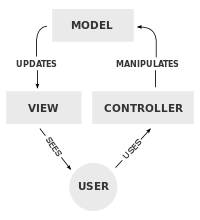
\includegraphics[width=0.5\textwidth]{model-view-controller}
 \caption{Model View Controller}
 \label{fig:model-view-controller}
\end{figure}

A native application interface is popular among server software and frequently used for desktop applications such as Microsoft Word and Microsoft PowerPoint but there has recently been a shift to using a thin-client\footnote{Use only to facilitate communication to a server}, running back-end\footnote{Main application logic} services in the cloud.

With modern networking speeds a user is typically unable to distinguish between running an application locally or interfacing with a remote server. \citep{schmidt1999interactive}.

By standardising the interface through an API, the user is also given the flexibility of using their preferred client, switching client without needing to worry about losing data and developers can design new interfaces without affecting and in parallel with the core application.

Users can also interact with multiple instances of the application running remotely. A feature particularly useful when running the application on a headless\footnote{With no monitors or peripherals.} server.

We must not neglect the benefits of using a native application. By making the UI interface with the application over the network, a whole host of complexity and security issues form.

The software needs to ensure that any user interacting with the API is authenticated and secure, as well as ensuring that there are no network issues between the interface and application.

The software itself also becomes more complex with a separate client as functionality needs to be built for handling network in both the UI and core application.

On balance, we opt for a separate interface. Membrane is a software daemon run constantly. In order to keep it lightweight and maintenance free we cannot run an interface that my use up a lot resources and get in the way for the user at the same time as the daemon.

The freedom of building additional interfaces to Membrane also helps extensiblity. Developers can easily tap into the API for additional interfaces making the requirement for both a GUI and CLI easy to fulfil.

\begin{figure}[t]
 \centering
 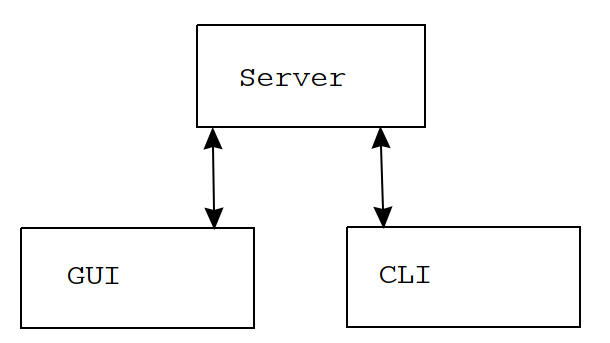
\includegraphics[width=0.5\textwidth]{client-server-model}
 \caption{Client Server Architecture}
 \label{fig:client-server}
\end{figure}

\subsubsection{Model View Controller (MVC)}

The Model View Controller (MVC) pattern, first described by \cite{krasner1988cookbook}, decouples the interface from the main logic of the program by establishing a subscribe-notify protocol between them. The view must always reflect the state of the model and the model must always update the view when a change occurs.

This approach allows for code-reuse and lets the developer to create new models without rewriting the software providing high cohesion\footnote{Groups of related actions are together}.

MVC has the disadvantage of making code harder to navigate due to added structural complexity, increasing scattering\footnote{multiple representations of objects need to be modified at the same time if required} and increases the learning curve for developers, as they need to learn how to structure the application in a new way.

Although the MVC model provides a structurally sound way of building the application we need to generalise in into the N-Tier architecture for larger applications.

\subsubsection{N-Tier Architecture}

An N-Tier architecture is simply an extension of the MVC model taking the idea of layers further. Sections of the software (or layers) can be developed and tested without interfering with each other.

A key advantage to this approach is extra layers can be added and removed, even during run time. In Membrane we will take advantage of this when running in Tracker or Local Backup mode. The Tracker can disable all of the local backup functionality as only the network layer will be required.

\begin{figure}[b!]
 \centering
 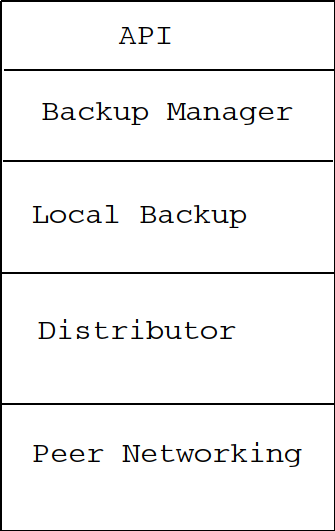
\includegraphics[width=0.35\textwidth]{membrane-n-tier}
 \caption{Membrane N-Tier Architecture}
 \label{fig:membrane-n-tier}
\end{figure}

We can see the Membrane N-Tier architecture in figure \ref{fig:membrane-n-tier}. Only modules next to each other are able to communicate directly and modules can be disabled as required.

The \emph{Local Backup} performs all the basic tasks of file monitoring and local shard storage. The \emph{Distributor} monitors the local backup for shards to send to peers and packages them up to the \emph{Peer Networking} layer for transmission. The Peer Networking layer is able to locate new peers and provides them to the \emph{Distributor} if connected.

\section{Technologies}

The technologies used in a project can define the success of a software project. Incorrectly chosen tools can slow development and be frustrating to use. While selecting technologies we will need to be weary of excitement surrounding modern technologies and look for unbiased advantages and disadvantages of each.

We will begin by selecting the language to use, followed by key libraries used within the software itself. Some of these libraries were chosen during development when the need for them arose.

\subsection{Languages}

A wide variety of languages are available for software development. We need to consider the best language for development of the Membrane Daemon, the GUI and the CLI. One of the most important features of a language is support from the developer community. An active developer community means any issues we encounter during development will most likely, already be solved by someone else.

We used the 2017 Stack Overflow Developer Survey \citep{stackoverflow2017survey} to find language popularity statistics. This is an annual survey held for users of one of the most popular developer forums covering everything from languages, to frameworks, to demographics.

\subsubsection{Daemon}

There are a few requirements when selecting a programming language for the daemon. The language must scale efficiently, restricting our choice to object-oriented languages. It must also be compiled, to reduce the chance of runtime exceptions the user would need to debug. Platform Independence is also key so Membrane can be easily ported to other platforms after the proof-of-concept is developed.

\subsubsection{JavaScript}

The most popular language by far is JavaScript, a high-level, dynamic, untyped language that is interpreted during runtime. \citep{flanagan2011javascript} It is one of the three core technologies used in the world wide web, the main driver of JavaScript's adoption. It has been standardised in the ECMAScript language specification, which has recently reached it's seventh edition. \citep{stefanov2010javascript}.

High-level languages uses strong abstraction to hide details of the underlying computer, such as memory management. This makes them easier to use and usually makes them much less bug prone.

Dynamic languages are a class of high level programming languages that execute behaviours usually performed at compile time in static languages, during runtime. \citep{trattdyamicallytypedlanguages} This typically means the language is dynamically typed (although not always). In the case of JavaScript, this is true.

An interpreted language is one for which most of the implementations execute instructions directly on the machine without compilation. The interpreter translates each statement into a sequence of subroutines that have already been compiled into machine code. In the case of JavaScript most of the runtime environments include a just-in-time (JIT) compiler, which compiles the program during runtime, dynamically recompiling and optimising frequently used code sections. \citep{aycock2003brief}

\subsubsection{Java}

We move onto Java, the second most popular (applicable) language. This is a general-purpose language that is object-oriented, class based and concurrent, \citep{gosling2014java} designed to run on all platforms that support Java without the need for recompilation. \citep{gosling1995java}

Object Orientation is a programming paradigm based on ``objects'' which contain data and methods that can act on that data. The class based aspect of java means that these objects are in fact instances of classes that determine their type. \citep{kindler2011object}

Objects offer encapsulation, an desirable feature that means they can only manipulate data inside them. This facilitates code refactoring, testing and encourages decoupling, which makes it very desirable for large software projects.

\subsubsection{C\#}

The final language we consider is C\#, which is another general-purpose programming language that offers strong typing, is imperative, declarative, functional and object-oriented. This makes it very similar to Java, and in fact has been criticised as a ``imitation'' of Java, although this has been disputed. C\# is a younger language than Java, so it was playing catch-up to Java's feature set for a long time, however, it has at this point surpassed Java. \citep{kreft2017afterjava}

On balance Java's popularity, larger community of users and open source nature means it is more suited to Membrane, although C\# has some clear advantages. Unfortunately C\# is not as well supported on Linux, requiring the Mono software platform to be run.

It is also important to take into consideration the ability of the developers coding Membrane, who have coded predominately in Java in the past.

\subsubsection{CLI}

We also need to consider the language to use in the GUI and CLI. For the CLI a fast, lightweight language is required. The three languages under consideration are Python, C and Go, selected because of their popularity, and the developer's familiarity with them.

\subsubsection{Python}

Python is a general purpose, dynamic, high level programming language. It is known for it's design philosophy which emphasises readability through forced indentation and a syntax tailored to representing algorithms in as few lines as possible.

This is a strong contender for the CLI, however, the most popular implementation of Python, \emph{CPython}, is a runtime interpreter making it slightly more difficult to ensure code correctness.

\subsubsection{C}

C is a general-purpose, imperative, statically-typed language developed in 1973 at Bell Labs. \citep{banahan1988c} It has become one of the most widely used programming languages of all time, providing low-level access to the hardware, and using language constructs that map efficiently to machine instructions requiring minimal run-time support.

One of the key disadvantages of C is that its power makes it easy to make mistakes. The low level access is not required for the CLI and it could potentially lead to subtle bugs.

\subsubsection{Go}

The final language, Go is a complied, statically typed language with garbage collection. It is designed to be scalable, not require IDEs\footnote{Integrated Developer Environment. A platform for developing.}, support networking and concurrency, and be productive and readable. \citep{golang2017faq}

This is a great compromised between the ease of programming in Python and the strictness found in C without sacrificing any of the benefits. Critics of Go say the lack of generics lead to some code duplication, but as the CLI will not require too much code, we are not concerned.

We also refer back to the Stack Overflow developer survey and see that Go is one of the most wanted and loved languages by developers, leading us to select Go for the CLI.

\subsubsection{GUI}

Finally a language for GUI development needs to be selected. This depends strongly on the choice of Electron for the GUI framework discussed in detail in section \ref{sec:gui-technology-choice}.

As we have selected a web technology we need to use JavaScript but there are two newer languages which transcompiles\footnote{Source code to source code compilation.} to JavaScript, enhancing JavaScript's feature set.

\subsubsection{CoffeeScript}

CoffeeScript aims to add syntactic sugar inspired by Python, Ruby and Haskell to improve JavaScript's brevity and readability. \citep{maccaw2012little} The compiled output is readable and tends to run as fast or faster as equivalent JavaScript. \citep{coffeescript2017faq}

There have been concerns using CoffeeScript adds bloat to development. Every change must be transcompiled before the effect can be seen, however, this can be solved by automating the process during development. Any time a page is reloaded, the server can automatically transcompile any modified CoffeeScript files to JavaScript. \citep{wheeler2017coffeescript}

Another concern is that using a transcompiled language makes debugging difficult as the debugger steps through a file that has been automatically generated for you, however, because the compiled output is intended to be readable, this has not caused issues for developers. \citep{wheeler2017coffeescript}

\subsubsection{TypeScript} \label{sec:typescript}

TypeScript is a super set of JavaScript developed and maintained by Microsoft as open source software. It is designed for the development of larger applications and aims to address the challenges of dealing with JavaScript code.

It supports static typing and adds features such as classes, modules and arrow function syntax, leading to better, more readable code. \citep{typescript2017site}

There are two major concerns with using TypeScript. To get the most out of TypeScript, developers need to add type annotations everywhere in their code, which makes coding a bit more cumbersome in comparison to JavaScript.

In addition, although TypeScript's type system is more flexible than mainstream statically typed languages, it still makes some common JavaScript software patterns difficult for developers to use. \citep{dataart2017site}

This is in addition to all of the considerations of CoffeeScript. On balance, we chose to use TypeScript for the Membrane GUI. The extra type safety provided outweighs the downsides of making it slightly more tricky to write the code. In addition if any quick coding is required, it is fully compatible with JavaScript so any sections of code unsuitable for TypeScript can be written using JavaScript seamlessly.

\subsubsection{Summary}

We have decided on three programming languages to use to create Membrane. Java, Go and TypeScript. These are three well-supported, popular languages best suited the developers coding the Membrane proof-of-concept to produce a stable and complete product.

Other languages including Bash, HTML, CSS, Python, Markdown, reStructuredText, and Groovy will be used during development, however, these are simply a requirement of the languages, frameworks and tooling chosen.

\subsection{Frameworks, Tools and Libraries}

To aid with development frameworks will be used. Some of these will be chosen at the before development, whereas other will be selected as a need for them arises.

\subsubsection{Java Build System}

There are three major build automation systems available for Java that help with application development, namely Ant, Maven and Gradle. These are responsible for compiling source code, running automated testing, detecting code coverage and packaging.

\emph{Apache Ant} was first released in 2000 and was the first modern build tool available for Java. It is able to accept plugins and is designed to have a low learning curve, enabling anyone to use it without special preparation.

Ant uses XML based configurations, to created build scripts, which is not ideal for writing the procedural scripts required. The use of XML also makes Ant difficult to use with larger projects. The build process is the biggest advantage of Ant.

\emph{Apache Maven} was released in 2004, designed to address problems developers encountered with Ant. Although it uses XML configurations like Ant it is better designed, relying on conventions and provides subroutines that can be invoked. Unfortunately the inherent downside of large build scripts remains.

One of the major advantages of Maven is the ability to download libraries and other dependencies over the network. Since this is the main purpose of Maven, custom build scripts are actually more difficult, however, these are not required by most users. \citep{viktor2014buildtools}

\emph{Gradle}, developed in 2012, is the most modern build tool and attempts to combine the power of both Maven and Ant. It uses Groovy (a JVM based language) for build scripts which results in shorter and clearer scripts, reducing the boilerplate required for creating basic configurations. \citep{gradle2017comparison} Gradle's flexibility is one of its major advantages. \citep{casperson2014comparison}

The two contenders for the build system become Gradle and Ant. Ant is preferred for developers new to build tools because of its low learning curve, however, as the developers creating Membrane have experience using all three build systems, we opt to use Gradle because of its clearer configurations.

\subsubsection{Java Networking}

The core feature of Membrane is it's ability to communicate with other peers. Using Java core networking libraries for this is an option, however, they provide an unnecessarily  low-level control over network communications. Use of these would no doubt result in reinventing one of the networking libraries available.

We look at three networking libraries in Java to see which is most appropriate for Membrane. One of the first requirements is the ability to send HTTP requests. These will be required for creating the API to interface with Membrane. Learning two networking libraries to develop Membrane would take more time with very little benefit.

The networking library of choice must also be able to establish SSL connections, which serve both the purpose of User Authentication and provide data security.

The contenders are Netty, Vert.x and Akka.

\emph{Netty} is a low level widely used library that promises quick and easy development without maintainability or performance issues. \citep{netty2017site} It is based around the reactor pattern to handle requests concurrently, and provides a wide variety of protocols for communication. It is more difficult to debug than traditional networking libraries because of the inherent concurrency, but has a wide variety of features and options.

\emph{Vert.x} is a polyglot\footnote{Multilingual.} library supporting seven languages including Java. It is built on top of Netty, focusing on a simple concurrency model, removing the complexity of debugging concurrent programs and has a simple asynchronous programming model to allow handling multiple requests at once. It aims to be a JVM alternative for Node.js, a popular JavaScript framework. \citep{vertx2017site}

\emph{Akka} is a library made for concurrent and distributed JVM applications. It draws on inspiration from Erlang for it's actor-based concurrency model, focusing on immutability and allowing actor interactions across multiple hosts when required. \citep{gupta2012akka}

We opt to use Vert.x in Membrane. It offers all the required features for peer networking with an appropriate concurrency model and without the complexity that comes from using a low-level library.

\subsubsection{Java Cryptography}

Security was a major concern for potential Membrane users and therefore the library we use for encryption needs to be selected carefully, again considering three contenders.

Membrane requires TwoFish encryption support and the ability to generate RSA public private key pairs and X.509 certificates\footnote{A way to present public keys for SSL}, as well as signing and authenticating messages using those keys.

\emph{Apache Shiro} is an open source security framework that offers authentication, authorisation, cryptography and session management, and aims to provide robust security while being easy to use. It was first released in 2010 and the latest release was 8 months prior to selection. \citep{apache2017shiro}

\emph{Bouncy Castle} is a collection of cryptography APIs for Java and C\# founded in May 2000. It is maintained by ``Legion of the Bouncy Castle Inc.'', a registered charity in Australia and prides itself on it's extensive test suite and standards compliance. It is by far one of the most popular cryptography libraries available. \citep{bouncy2017castle} The latest release was two months prior to selection.

\emph{Keyczar} is a newcomer created by Google, aiming to make it easier and safer for developers to use cryptography in their applications, providing simple one line cryptography functions to developers instead of being a general-purpose cryptography library. It was first released in 2010 and the latest release was one month prior to selection. \citep{keyczar2017github}

Shiro is a good option, however, it provides a lot of unnecessary features. It's focus is not aligned with the requirements of Membrane. Keyczar is a good library for limited use-cases.

We find that Bouncy Castle offers the best feature set. It is the oldest library by far, and it's popularity during that time makes it much less likely to have bugs.

\subsubsection{Version Control} \label{sec:versionControl}

Version Control is an important aspect of any software project. During selection we focus on the extensiblity requirement, which requests easy contribution for other open source programmers.

There are two leading platforms \emph{Github} and \emph{Bitbucket}. We opt to use Git for version control because of it's clear advantages, allowing for decentralised version control while working from multiple workstation, over competitors such as SVN and CVS.

\emph{Github} was launched in 2008. Offers code review, issue tracking, documentation, wikis, pull requests and releases. It has 5.8M active users and 19.4M active repositories. \citep{github2016octoverse} offering multiple integrations for continuous integration and code quality analysis. It also offer public repository hosting for free.

\emph{Bitbucket} was launched at the same time as Github in 2008 and started only hosting Mercurial projects but quickly expanded to Git as well. \citep{bitbucket2017site} It's main advantage is it's close integration with JIRA, a popular issue tracker. \citep{upguard2014gitvbit}

On balance, given the popularity and available integrations, we opt to use Github for version control. We use four Github integrations in the project.

\emph{TravisCI} offers continuous integration, running testing on all targeted JVMs after every commit and notifying developers if a test fails.

\emph{VersionEye} ensures that all external dependencies used are up-to-date and have no security flaws.

\emph{CodeCov} automatically checks test coverage for every commit, warning the developer if coverage is decreasing due to the commit.

Finally \emph{rtfd.io} provides documentation for the project, building a hosting documentation from the project source code.

\subsubsection{Other Libraries}

We use \emph{Google Guava} and \emph{Apache Commons Collections} to enhance the standard Java libraries, offering a wider range of functions and desirable features such as immutable collections.

For marshalling\footnote{Converting objects to text and back.} data we opt to use \emph{Jackson} for data transmission and local storage. It can serialise objects to both JSON and YAML. Advanced date functionality is added using \emph{Joda} and finally \emph{Junit Jupiter} in conjunction with \emph{Mockito} will be used for unit testing.









\chapter{System Components}

The components that make up Membrane are all designed individually and connected using Java interfaces. In this section we discuss the goals and functionality of each, explaining decisions taken in the final architecture of Membrane.

We begin with file ingestion and file system monitoring, file storage and peer appraisal. Then we determine which peers are most appropriate to hold which files and finish on networking, covering the details of authentication and security.

\section{File System Monitoring}

Monitoring the file system for local changes is key to any backup system to be able find new files to preserve. In this section we design a method to watch specified folders for these changes. First we explore methods of walking the file tree, used when the user specifies folders using wildcards\footnote{Which can be used to signify arbitrary folders} or asks to include inner folders.

We take two approaches to watching folders and discuss augmentations made to the chosen technique, ending the section by discussing methods of deduplication for repeated files and future enhancements that could be made to the implemented monitor.

\subsection{File Tree Walking}

We allow users to select folders for backup in three ways: explicitly, using wildcards\footnote{Added using a \code{*}.}, and recursively. When allowing users to specify folders recursively we must inspect the contents of the folder and visit each inner folder, determining if it is suitable for monitoring as shown below. This can be achieved using the visitor pattern in Java which lets us recursively visit each folder in base folder given to either mark or discard the folder. \citep{sugrue2010visitor}

\begin{displayquote}
 User entry (recursive): \code{/tmp/AA/BB/*/CC} \\ \\
 Matches: \code{/tmp/AA/BB/any-folder/CC} , \code{/tmp/AA/BB/any-folder/CC/FF}\\
 Does not match: \code{/tmp/AA/CC/any-folder/CC}
\end{displayquote}

Once all of the relevant folders are found we begin watching them for changes. We need to remain aware of folder additions or deletions and keep the list of watched folders up-to-date accordingly. Folders specified using wildcards might not necessarily be created in already watched folders so these folders must be manually scanned on a regular basis.

When finding folders it is important to note the difference between a file, folder, hard link and soft link (also known as a symlink or symbolic link). To understand these we must first observe how files are stored in a Unix-style file system, which supports ordinary files, folders and special files.

Index Nodes (commonly refereed to as inodes) are items\footnote{Data or metadata} in the file system stored by a unique number. Directories provide a way to structure and name these inodes by containing a list of files (references to inodes). Each file is mapped to exactly one inode, and each inode can have more than one file mapped to it. \citep{bar2001linux}

A hard link is an inode that has multiple names in the file system. These need to be deduplicated with Membrane, however, this is encompassed within the general deduplication mechanism implemented.

A symlink is formally any file that contains a reference to another file or directory which will affect path name resolution\footnote{The act of finding a file given a file path.}. The symlink is an inode that exists independent of the target inode and simply forwards any requests to the target. If the target is deleted or moved it continues pointing to the same (now invalid) location. \citep{yue2011unix}

Symlinks are a useful tool typically used to link different file systems, but they complicate file tree walking by changing the file system from a tree into a directed graph with loops.

Within Membrane we opt to ignore symlinks while walking the file tree. Users are able to specify the target directory of the symlink separately if required. Symlink deduplication is handled by a higher level mechanism, just as with hard links.

\subsection{Polling}

A naive method used to check folders for file changes is simply periodically scanning the folder, finding differences between consecutive scans. The modification time stamp of the file (provided by most modern file systems) can be used to determine if existing files have changed in the time.

This simple method is very expensive, consuming a lot of memory as it needs to retain a copy of the last modification date and all of the files in the watched folders.

This method is also IO intensive. The file listing in the directory on the file system contains no metadata, so every single inode in the folder needs to be accessed to gather its metadata. This primarily affects users using storage media with poor IOPS\footnote{Input-output Operations Per Second} common in hard disk drives. As the impact may not be observed on more modern computers it is important to consider this before deployment. \citep{mansurov2017storage}

Polling is a poor solution for Membrane. During user surveys low resource usage was requested so periodic spikes in IOPS that may adversely impact other applications are undesirable.

\subsection{Native Watching}

File Change Notifications (FCNs) are a more advanced method of watching files built into some file systems. FCNs are sent out to subscribed services when an inode changes and are used in three common scenarios \citep{kerrisk2014fcn}:

\begin{itemize}
 \item When creating a model of the file system.
 \item When logging file system activity.
 \item In gatekeeper services that ensure only permitted operations happen on the file system such as an anti-virus.
\end{itemize}

We want to use FCNs to both model the file systems internally within Membrane and to log activity in order to reproduce historical versions of the file system.

The first implementation of FCNs, \emph{dnotify}, appeared in Linux in 2001. It suffered from a cumbersome API and most notably, it kept file descriptors open causing problems when trying to unmount file systems. \citep{kerrisk2014fcn}

The inotify API was released in 2005 and aimed to address all of the issues in dnotify. It consists of three dedicated system calls \code{inotify\_init()} which maintains a list of file system objects that should be watched and a list of events generated for those objects and the commands \code{inotify\_add\_watch()} and \code{inotify\_rm\_watch()} are used to alter the list of monitored file system objects. inotify provides more information than dnotify, allows programs to deal with notifications synchronously and includes the file name modified. \citep{kerrisk2014fcn}

Java implements the \code{WatchService} API which provides low level access to the underlying inotify API of the file system. \citep{oracle2017dir} We opt to use this when the API is available, but fall back to polling when inotify or similar services are unavailable.

\subsection{Watching Enhancements}

Despite the comprehensive feature set of inotify, we still require some enhancements to prevent FCNs missed during application down time and FCN buffer overflows\footnote{inotify can only store a limited number of transactions between scans}. 

Between application runs we need to load all known and expected files into memory and scan the file system on first load. This means resorting back to maintaining a list of all monitored files in local memory, an unfortunate but necessary step.

We now match any reported modified or deleted files against the internal state, using the modification date and hash of the file to determine if the file has been changed. In order to lower resource usage we read any modified files in sections, never loading more than 4MB into local memory. These chunks become shards within the backup system.

\subsection{Deduplication}

There are two viable approaches to file deduplication for Membrane. We can choose to split the file into shards and check if shard hashes match, or use a rolling checksum, similar to Rsync to find which section of the data has changed. \citep{tridgell1996rsync}

Simply splitting the file into chunks has the disadvantage of being unable to detect overlapping data, which can lead to large amounts of accidental duplication. When data is inserted into the middle of a file any blocks after and including the change will be marked as modified and need to be restored.

The approach of simply sharding the data is simple and much less prone to bugs, so we take this approach with the initial implementation of Membrane, although we will maintain support for variable size chunks for future implementations. This is a compromise taken to lower development time for proof-of-concept.

A method of generating a unique hashes for file shards is also required. Git and Subversion opt to use SHA1 \citep{torvalds2010git} to generate unique keys for files, however, we also consider MD5 for this purpose.

Both SHA1 \citep{wang2005collision} and MD5 \citep{stevens2006fast} are cryptographically broken, meaning that it is possible to generate a collision\footnote{Two different inputs producing the same hash} without having to try every possible input into the hashing function. It is also possible to launch a first preimage attack on these hashes, something that would make them unusable for security as an attacker would be able to generate an input matching any given hash. As Membrane only uses this hash as an internal shard identifier, we do not have to be concerned about an external attacker.

The only situation in which this may cause issues in the future is if the user stores two shards with the same hash accidentally, however, the chances of that are small enough that it is not worth worrying about. In this unlikely scenario Membrane would simply reject the newer shard causing the new file to be corrupted when a reconstruction is attempted. This was discussed in detail by \cite{torvalds2006gitcollisions} and other git developers. An inadvertent collision was deemed so unlikely that it was reasonable to use SHA1 for Git.

MD5 only has a 128 bit output vs. the 160 bit output of SHA1, meaning collisions are slightly more likely, however we mostly concerned about hashing speed, seeing as this hash will be run very frequently on any files that have been altered, and studies have shown that MD5 is on average about 1.75 times faster than SHA1. \citep{saphir2007securite}

We calculate the probability of a collision by using a solution to the generalised birthday problem, which measures the probability of two objects having the same identifier given $d$ identifiers and $n$ objects.

$$p(n, d) = 1 - \frac{d!}{d^{n}(d - n)!}$$

As we are working with very large numbers we use an approximation provided by \cite{brink2012probably} that is proven to hold within 1\% for all $d$ up to $10^{18}$, which would be four yottabytes\footnote{A yottabyte is $2^{80} bytes.$}, an incomprehensibly large amount of data:

$$p(n, d) \approx 1 - \bigg(\frac{d-1}{d}\bigg)^{n(n-1)/2}$$

Assuming users will store no more than 2TB of data in 4MB shards (resulting in $5 \times 10^5$ shards), we find the probability of a collision is $1.47 \times 10^{-29}$.

Accepting users might like to backup 40TB of data the shard count increases to $10^{7}$. The collision chance still remains at an insignificant $1.47 \times 10^{-25}$.

In the future we can always convert to SHA1 which would provide a collision probability of $3.42 \times 10^{-35}$ at 40TB.

\section{Local Storage System}

As Membrane is a backup system it needs to store a log of file activity containing file meta-data and contents of each version of that file. In this section we discuss the shard storage mechanism, file history persistence and finish on the file history expiration policy used in Membrane.

\subsection{Shard Storage}

When a file change is detected the watcher shards the file into 4MB chunks and sends them directly to shard storage. The shard store manages a folder of the file system and provides functions for shard storage and retrieval, similar to those found in block storage services offered by cloud companies to allow for future integration.

When a shard is inserted into storage the file system first checks if the shard is already stored. If so the shard is ignored altogether and the write is avoided, saving disk IO\footnote{Input or Output operations, a limited resource on computers.}. Otherwise the hash of the data is confirmed and the shard is written to a file on the disk.

Because of file system limitations we use a hierarchical directory structure for storing shards. A new directory is created every five characters of the shard as shown below overcoming any restrictions on the maximum number of files per directory older file systems may have, such as ext2 and ext3 which reportedly have performance issues with anything above $10^5$ files. \citep{johnson2014files}

\begin{displayquote}
 \code{Shard [kt903hbt7h24p7h32] -> directory/kt903/hbt7h/24p7h/32.mem}
\end{displayquote}

The shard storage runs scrubbing on a regular basis, a concept taken from the ZFS file system \citep{oracle2012zfs}, periodically checking that every shard stored is consistent with its hash and is actually accessible. This is a technique commonly used to prevent errors before they result in failure, complimenting shard integrity verification during reads by proactively removing damaged shards.

\subsection{File History Storage}

The file history is the central store of the backup system. It contains a log of every file addition, modification and removal providing all of the information required to retrieve it. It is important that the store is immediately persisted to the file system upon backup so nothing is lost during unexpected shutdowns.

The naive approach uses a log implemented in the form of a linked list to record events flushing new entries immediately to a log file. Although this approach satisfies all of the requirements it is very expensive to search and quickly becomes very large.

Taking inspiration from distributed file systems such as HDFS \citep{hdfsAnalysis} and GFS \citep{mckusick2010gfs} which use NameNodes to store file system modification in a checkpoint and journal. The journal is a write-ahead commit log that takes the place of the aforementioned event log. The checkpoint is a known file system state. In the event of system failure these file systems can replay the log, starting from a persisted checkpoint to recreate the state during power loss.

Within Membrane we use checkpoints as a method of memoization\footnote{Caching results.} to speed future searches through the journal. The start and end of the journal are queried so often they are given special permanent checkpoints that are always kept up to date.

\begin{figure*}
 \centering
 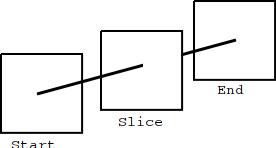
\includegraphics[width=0.35\textwidth]{journal}
 \caption{Storage Journal - Journal (line) with start, end and requested time slice}
 \label{fig:journal}
\end{figure*}

When the user queries for a specific point in time, the journal can be replayed from the closest memoized checkpoint to the requested time, quickly generating the state of the required time slice. A visualisation of this is shown in figure \ref{fig:journal}.

This proved to be an effective way of storing file history, providing quick responses to the GUI, CLI and other system components, even when full of data. If this proves insufficient for future demands. In order to help speed queries the journal can also be indexed to see every file that uses a shard.

It is important to address the distinct lack of a transactional database in a situation where the use of one seems like a natural fit. Traditional databases such as MySQL have very high memory and CPU usage, \citep{james2017sql} and although this usage can be tuned running a full database on a users computer would go against the resource usage requirement.

\subsection{Backup Management}

One of Membrane's proposed features is flexible file history. Instead of providing a backup storage duration, backups are stored until the space allocated to Membrane is completely used.

This is a step towards the maintenance free experience requested by survey participants. Many cloud solutions such as \cite{dropbox2017versions} allow users to access version history for a set amount of time, requiring extra subscriptions for additional versioning time.

In order to implement this we take the concepts used in garbage collection (GC) within programming languages and apply them to the file history. In addition to a maximum shard storage size, a target size is set.

The monitor adds shards until the maximum limit, ignoring the target size. If the storage reaches the maximum limit GC is called, compacting the file history and removing dereferenced shards. The GC is also called periodically to avoid the watcher having to retry writes due to hitting the maximum limit.

GC is a three step process that attempts to reach the target storage size in the least destructive way by:

\begin{enumerate}
 \item Garbage Collection
 \item Remove Unwatched Files
 \item Trim Older Journal using FIFO
\end{enumerate}

Garbage collection is implemented using an adapted version of \cite{dijkstra1978fly}'s mark and sweep algorithm. This works in three passes. 

\begin{enumerate}
 \item Certain shards are protected from garbage collection as they have just been added into shard storage and might not have their reference inserted into the journal yet, generating set $P$.
 \item The second pass walks the journal and collects shards mentioned in the journal creating set $R$
 \item The final pass finds $S \setminus (P \cup R)$ where $S$ is the set of all stored shards, and removes them.
\end{enumerate}

This step is intended to remove any shards that were inserted into shard storage but never followed up with a file entry, possible in the case of error during shard storage or file history storage. The implementation for garbage collection can be found in listing \ref{lst:fileGC}.

The next step is intended to remove any entries the user is not interested in any more. These could have been inserted after recovery from peers or may have been files that were temporarily backed up. If any files were deleted garbage collection is re-run to remove the relevant shards.

Finally the journal is trimmed, removing any history necessary. The algorithm creates a shard count dictionary to see if removing the last file in the log will affect the storage. If it does it is removed, otherwise the algorithm moves along to the next entry. This is repeated until the target storage size is reached. The method used means no file entries are unnecessarily removed. The implementation can be found in listing \ref{lst:storageClamping}.

\subsection{Local Backup}

With both the local storage system in place and file system monitoring, we have developed a full local backup system. Files are detected by the monitor, split into shards, which are stored in shard storage, and the modification event is stored in modification history. Available files, file history and file version recovery can be requested and completed successfully.

The components described hereafter can be completely disabled for a local Membrane installation. We next describe the Application API, which allows the user to interface with the daemon.

\section{Application API}

As extensiblity is a requirement for Membrane, it is paramount that the application API is robust and assists future developers with interactions. We look at \cite{google2017api}'s and \cite{heroku2017api}'s API design guides to form a coherent and sensible set of requests and responses for developers. The design of APIs is very important in Software Engineering and the final result can have significant impacts on usability. \citep{benslimane2008services} 

\subsection{API Type}

There are there main types of APIs considered in API design. \citep{boyd2017api}

\begin{itemize}
 \item Open - Public expose information and functionality
 \item Partner - Used for integration between a company and it's partners
 \item Private - Only used internally to facilitate communication.
\end{itemize}

The Membrane API is a private API as only the user will be permitted access. We opt to authenticate the user by using a source IP filter. Only interactions from the loopback address\footnote{An IP address that connects from the host itself. \citep{hinden2006ip} It is infeasible to send a request from this address unless it originates from the user.} $127.0.0.1$ will be permitted. This decision makes development easier and fulfils all of the proof-of-concept requirements, but it can always be expanded if the need to access the Membrane API remotely arises.

As discussed previously, we opt to use a Representation State Transfer (REST) API. In web development, an API is typically a set of Hypertext Transfer Protocol (HTTP) request messages, with defined responses in either Extensible Markup Language (XML) or JavaScript Object Notation (JSON). We opt for JSON within Membrane because XML is more difficult to parse and JSON is shorter, quicker to read and write and can use arrays.

In the past Web APIs were typically Simple Object Access Protocol (SOAP), which focused on providing access to services. \citep{benslimane2008services} More recently REST APIs, more focused on resource access have gained popularity. These aim for fast performance, scalability, simplicity, easy modification, communication visibility, portability and reliability. \citep{fielding2000architectural}

There are five main guiding constraints to building a RESTful API \citep{fielding2000architectural}: 

\begin{itemize}
 \item Client-server - By separating the user interface concerns from data storage concerns, portability across platforms is improved. In addition components can evolve independently and be in differing states of completion.
 \item Stateless - All the information required for a request is contained in one request. This reduces the need for persistence on the server side.
 \item Cacheable - Any intermediaries can cache a response to improve responsiveness, and responses must be marked as cacheable or not.
 \item Layered System - A client should be unable to tell if an intermediary is passing it's data. This improves potential scalability.
 \item Uniform Interface - This decouples the underlying architecture from the interface allowing both to evolve independently.
\end{itemize}

All of these properties are desirable within Membrane for limiting resource usage and allowing future expansion. This in addition to the vast amounts of tooling created to assist with RESTful API development such as \cite{postman2017api}\footnote{A tool for manually making REST calls}, means that we opted for a RESTful API within Membrane.

\subsection{API Design}

We now need to structure the API. There are five available HTTP methods emph{POST}, \emph{GET}, \emph{PUT}, \emph{PATCH} and \emph{DELETE} which can all be used to invoke actions on the server side.

We opt to split our requests into three categories `\emph{status}', `\emph{configure}' and `\emph{request}' to keep the API simple, intuitive and consistent, as recommended by \cite{google2017api}.

Simple status updates are available under `\emph{/status}'. The status is split into four modules of membrane: `\emph{network}', `\emph{storage}', `\emph{watcher}' and `\emph{contract}', such that a GET request to `\emph{localhost:13200/status/watcher}' would return JSON information regarding the file watcher. In the future we plan to further subdivide the API in case specific information is required, to reduce the amount of calculations required on the server side per request.

Calls to Membrane regarding configuration are grouped under `\emph{/configuration}'. Here the client needs to provide request information using the URL or accompanying data. Although using URLs is useful, this may cause issues in the future when inputting folders that use the same file separator as URLs. We opt for \cite{heroku2017api}'s suggestion to request JSON data structures. We return HTTP status codes to indicate the result of the request, compliant with RFC7231 \citep{fielding2014hypertext} as per \cite{google2017api}'s recommendation.

Last of all we require users to send requests to Membrane for file history and file recovery. Here we use both JSON POST requests and responses.

An important part of API design is human-readable documentation, so future developers can understand the API. \citep{heroku2017api} We have created documentation for the Membrane API, made available both in listing \ref{lst:apiDocs} using the reStructuredText markup language and at \url{http://mbrn.rtfd.io} using version controlled documentation generation available via Github, first mentioned in section \ref{sec:versionControl} when selecting Github.

\section{Shard Distribution}

Membrane is a peer-to-peer file backup platform. In the previous three sections we have created a functional local backup application for users wishing to backup and version file to a local storage medium, such as a removable hard drive. The following two sections focus on taking that data, securing it and passing it to peers for remote storage.

There are two important data stores that need to be distributed, the file history containing metadata required to reconstruct files and shard storage containing the data used for file reconstruction.

In this section we assume we are subscribed to a feed of peers we can send messages to. We first discuss storage blocks, the mechanism for packaging shards and metadata, followed by the contract system employed, concluding with the peer appraisal trust system applied.

\subsection{Shard Packaging}

In order to start trading data with peers a standardised container for shards needs to be created. The only limitation imposed is the size of the container. For Membrane we decide through empirical testing, a container size of 25MB is a good size. This number allows the storage of six full 4MB data shards, leaving 1MB for any any metadata required. It is also small enough that we can store multiple copies in-memory for data manipulation and in the write buffer while sending.

Each container, hereinafter refereed to as a \emph{block}, requires overhead for transfer and proof-of-existence discussed in the following section (\ref{sec:contractMech}), so it is useful to select as large a size as possible. We show a typical block diagram in figure \ref{fig:storage-block}.

\subsubsection{Compression}

When crafting a block for a potential peer, shards that the peer has not yet stored are selected. Membrane then attempts to compress these shards, some shards might not be compressible\footnote{As the data may have difficult to detect patterns.} and in that case we flag the shard as uncompressed.

We first implement Snappy due to very small amount of development time required, as discussed in section \ref{sec:compression}, and later added LZ4\_FAST compression as we had time to improve the feature. We add metadata about the compression algorithm used in the block data, so new and better compression algorithms can be added in the future, in line with the extensiblity requirement.

\begin{figure*}
 \centering
 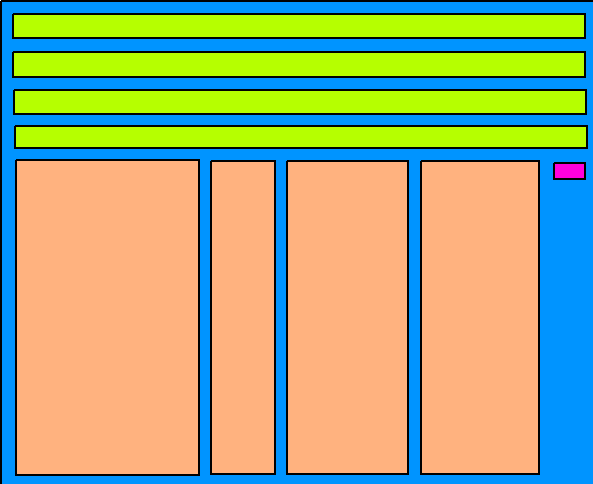
\includegraphics[width=0.5\textwidth]{storage-block}
 \caption{Storage Block - Shards (Orange), Metadata (Green), Free (Blue), Salt (Pink)}
 \label{fig:storage-block}
\end{figure*}

It is imperative the compression is performed before encryption as encrypted shards are made up of pseudorandom data. If the encryption algorithm follows \cite{shannon1945mathematical}'s laws of confusion\footnote{Each bit of the ciphertext should depend on several parts of the key} and diffusion\footnote{If a single bit of the plaintext or ciphertext, is modified then half of the bits in the ciphertext or plaintext should change respectively}.

\subsubsection{Knapsack}

To fit data in the block we are faced with the knapsack problem. This is a packing problem commonly encountered in Computer Science. \citep{skiena1999interested}

Given a maximum container size $W$ and a set of $n$ items, shard sizes in our case, each with a value $v_i$, size $s_i$ and size we must find the set 

$$\max \sum_{i=1}^{n} s_{i}x_{i}$$ 

such that 

$$\sum_{i=1}^{n} s_{i}x_{i} \leq W, x_i \in {0, 1}$$

This is an NP-Hard optimisation problem, \citep{skiena1999interested} meaning it cannot be solved in polynomial time. We are faced with the additional issue, that we do not know the size of all the shards without accessing the inode of the shard, a comparably expensive operation. There are pseudo-polynomial\footnote{Running time is polynomial in the numeric value of the input (container size in this case)} time algorithms that can solve the problem but without all of the sizes available we cannot fully benefit from them.

We attempt to solve the solution by simply looking at a subset of $100$ random shards from the queue and using the dynamic programming solution with $O(nW)$ computational and space complexity. \citep{martello1999dynamic} We lower W to a reasonable level by dividing all weights by 128kB. This gives a maximum of: 

$$(25\mbox{MB} / 128\mbox{KB}) * 100  \mbox{ shards} = 2000 \mbox{ loops}$$ 

which is far superior to the $n! = 100!$ naive solution. The code for this is available in listing \ref{lst:shard2block}. Although we are able to fill the block optimally for those 100 shards, it causes starvation for blocks sized between 1MB and 4MB.

Blocks of size 4MB filled the 25MB space until there was 1MB left, which was filled by shards of size $\leq1$MB. Shards between 1MB and 4MB were rarely selected as blocks of size 4MB and $\leq1$MB were quickly replenished.

We therefore opt for the naive approach of filling the blocks in FIFO\footnote{First In First Out}, skipping a shard and moving to the next one if it no longer fits, up to 100 shards.

When tested over a standard set of sharded files taken from the document directory of three users with compression disabled, the packing efficiency was $0.90$ with a standard deviation of $0.026$. Raw data is available in table \ref{tab:storageUsage}.

The maximum inefficiency we can observe is if the block has just under $4MB$ remaining with only $4MB$ available. This results point reaching an efficiency of approximately $21/25 = 0.84$. This leaves the expected average efficiency at $0.92$, is within margin of error the result. 

An advantage to this naive solution is we can consider the remaining space after compression. Something that would require compression of all the blocks first in the knapsack algorithm.

In the future we may attempt to find a better solution to this problem, perhaps by favouring shards that have not been uploaded for a longer time. It is important to also remember that if all peers create blocks of the same size, then the system remains in balance. This could be exploited by another client with more efficient packing.

\subsubsection{Adding metadata}

Once the block is fully packed with shard data, we place the file history for every shard in the block ensuring, that if data is lost and the block is returned, Membrane can reconstruct files as soon as possible.

We then insert a randomly generated salt into the block. This is small, however, because of the aforementioned law of diffusion \citep{shannon1945mathematical} this should lead to completely different encrypted data. This is done to ensure that the same block is never sent out twice, a requirement for proof of ownership in section \ref{sec:contractMech} that prevents one peer being able to issue proof of ownership on behalf of all peers holding the block.

We finally encrypt the shard using a SHA-256 hash of the private key used by the Membrane networking module. Twofish encryption is used, as decided in section \ref{sec:encryption}. The block is now ready to be sent to the peer by the contract mechanism.

\subsection{Peer Contract Manager (PCM)} \label{sec:contractMech}

In the literature review (\ref{sec:neg}) we explored contract negotiation within intelligent agents. Many contract negotiation techniques studied require multiple steps to come to an agreement. We hope to implement a pragmatic heuristic approach to shard allocation that does not require complex negotiation, relying on peers to offer storage for free in the hope other peers will do the same. We now describe an overview of the contract mechanism, followed by an in-depth analysis of why it works.

As in Game Theory, we assume all Membrane peers are entirely self-interested. The main purpose of the peer is to distribute blocks and the only way to achieve that is by becoming attractive to other peers for block storage. This can be done by correctly storing blocks for them. This system does not depend on altruistic behaviour, instead making good behaviour the only way to benefit from the system.

\subsubsection{Contract Update}

A contract update is the only method a PCM can change the state of a contract for a peer. It is a statement of fact indicating two things:

\begin{itemize}
 \item An integer permitted inequality. (The peer can store this many more blocks with you, than you have stored with it.)
 \item List of Blocks you are holding for the peer.
\end{itemize}

Updates are sent whenever a peer is contracted, connects, a new block arrives from the peer and every 15 minutes. To be marked down as available during that hour of the week a peer must send a contract update that hour. These marks are then used to calculate appraisal, discussed in section (\ref{sec:peerAppraisal}). To remain contracted a peer needs to maximise their appraisal.

\subsubsection{Contracts}

Contracts are Service Level Agreements (SLAs) within Membrane. When you give a peer an offset, you sign a SLA declaring you will:

\begin{itemize}
 \item Accept and store blocks from the peer (up to the amount the PCM is holding for it, plus the offset)
 \item Send Contract Updates at least once every hour while the SLA is active.
 \item Complete Block Instructions issued by the PCM - Used for proof of existence and block management.
\end{itemize}

We apply four sections of \cite{keller2002defining}'s SLA life-cycle to these contracts, the contract update allowing for three of the four life-cycle stages: Establishment, Reporting and Termination. A peer is only able to provide verifiable facts in the contract update, so it is impossible for peers to be deceitful.

The offset can be modified as required throughout the SLA, with 0 terminating the SLA. Upon termination all blocks stored for the peer are removed.

\subsubsection{Block Instructions}

Upon receiving a contract update the PCM sends one of the following block instructions (also referred to as evidence requests) to the peer.

\begin{itemize}
  \item Compute Evidence for the Block
  \item Remove the Block
  \item Send the Entire Block back
\end{itemize}

There are six possible scenarios for each block sent in the contract update.

\emph{Lost Blocks} are blocks the PCM expects the peer to have that they did not report in the CU. The block is removed from the contract and the violation is marked in the peer appraisal.

\emph{Unexpected Blocks} are blocks not in peer contract. These are temporarily\footnote{Not influencing how much space the PCM offers the peer.} inserted into the peer contract. The entire block is requested.

If the peer is truthful, the block will be correctly decrypted and lost shards will be recovered. In the next update the block will register as expired. Otherwise this will be noted as a block loss. It is therefore in the peers interest not to make up fake blocks.

\emph{Required Blocks} contain shards that are not present in local storage. These are requested for recovery.

\emph{Proven Blocks} are blocks that have already been verified this hour and are not required, these blocks are ignored with no block instructions sent.

\emph{Provable Blocks} need to be verified for a good peer appraisal score this hour. There are three ways to prove you own a block to a peer (\ref{sec:pdp}). A block instruction contains the capability of sending a short salt for this purpose.

\emph{Expired Blocks} have no salts available for proof or contain no active shards. These are removed.

If the peer correctly responds to all of these messages it will have verified all of the blocks it claims to own, increasing its attendance for the hour score and making it a more likely choice for the PCM to store blocks with.

If a peer does not verify all the blocks it declares by the end of the hour a severe penalty is applied to the appraisal rating for the peer.

\subsubsection{New Peers}

The PCM has a target number of peers that it should share blocks with. When a new peer arrives before that target is reached the PCM offers an offset of one to that peer. This qualifies as a contract modification so a contract update is sent to the peer, giving the peer an all clear to start sending blocks.

\begin{figure*}[h]
 \centering
 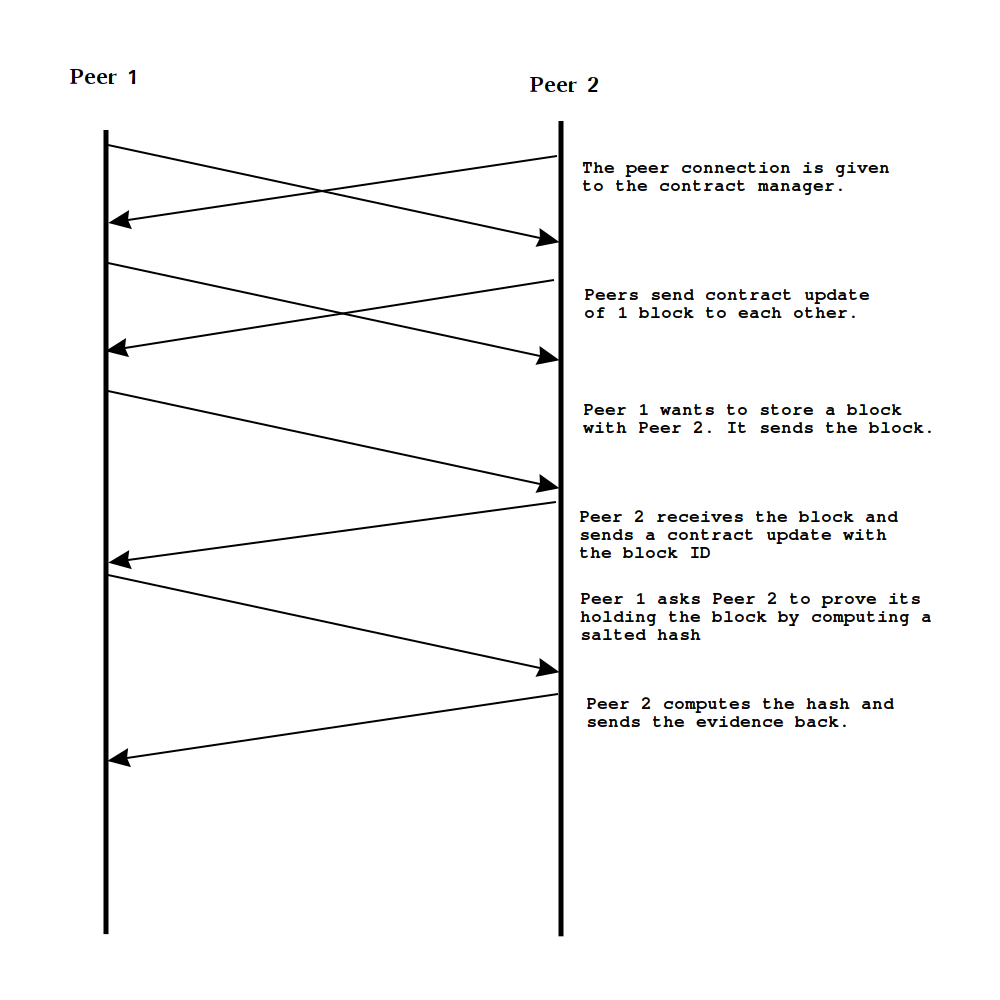
\includegraphics[width=0.8\textwidth]{contract-start}
 \caption{Peer Contract Start Example}
 \label{fig:contract-start}
\end{figure*}

We expect a similar contract update, marking the start of a contract from the peer. We stop any incoming blocks from peer that have not given us any space to store with them. This would be an unfair deal that we are not interested in. The mechanism can be observed in the initial part of fig \ref{fig:contract-start}.

\subsubsection{Provable Data Possession (PDP)} \label{sec:pdp}

To allow the peer to prove they own a file the PCM calculates a set of salts and resultant HMACs for each block deployed as described in section \ref{sec:poo}. One salt and HMAC pair for each hour for the two week lifetime of the block.

We opt for the Keccak hash function, developed by \cite{bertoni2009keccak}. It used in SHA-3, a cryptographic standard released by NIST in 2015 \citep{paul2015nist}. There are no known exploits for Keccak and we use the 512-bit variant recommended by \cite{bertoni2009keccak} in 2013.

We take advantage of the fact that there is no known way to compute a HMAC without both the data and the key. As the PCM releases the key during the hour the peer is verifying the data, the PCM can be certain the peer held the block at that point in time. \citep{ateniese2011remote}

In order to prevent all the stored blocks being loaded by the client the PCM has a 50\% probability generating an empty key (except for the first and last proof), requiring no calculation by the peer. There is no way to predict this and therefore no way to abuse this feature. This is a pragmatic, very solution specific way of reducing IO required for PDP as the peer pays a huge reputation penalty for losing a block. There are more advanced methods that can be investigated \citep*{ateniese2011remote, shacham2008compact, bowers2009proofs}, however, we opt for this solution in this proof of concept system.

We also need a demonstration that the peer will send us the full block on request. We request that 1\% of the time, instead of sending a salt and KMAC computation request, the whole block is request.

When there are no more salt and KMAC pairs that the block is marked as expired and removed during the next contract update.

We do not use Keccak Message Authentication Codes (KMACs), a newer more efficient keyed hash function that makes use of the sponge construction of Keccak to only hash once \citep{kelsey2016sha}, as the standard is new and the cryptography library we use does not support it yet.

\subsubsection{Contract Scaling}

To accelerate block trading with favoured peers for every 10 blocks traded, the PCM increases inequality by one, allowing for more flexibility and faster growth. We choose a linear scaling system as the space made available to the peer must actually be available. Growing exponentially would quickly give the peer more space than we have available. 

The maximum amount of blocks transferred to each peer per upload is capped at six. This is due to a buffer limit of 256MB by the networking layer. If we assume all blocks are full and accounting for base64 encoding used for transfers, we find that this gives space for $(256 * \frac{3}{4}) / 25 = 7.68$ blocks. Room is left for potential messages between clients while blocks are transferring.

The contract scaling allows adding friends in future expansions. A user can manually select a peer and increase their inequality, gifting them block space. We do not provide an interface to this in the proof-of-concept implementation of Membrane.

\subsubsection{Complete Data Loss Scenario}

In the case of data loss the PCM is empty containing no contracts. Previously contracted peers locate the new PCM instance using PEX, unaware of the data loss. Contract updates are exchanged informing the peer that the PCM no longer holds any of their blocks, and the PCM treats all of the received blocks as lost.

\begin{figure*}[ht]
 \centering
 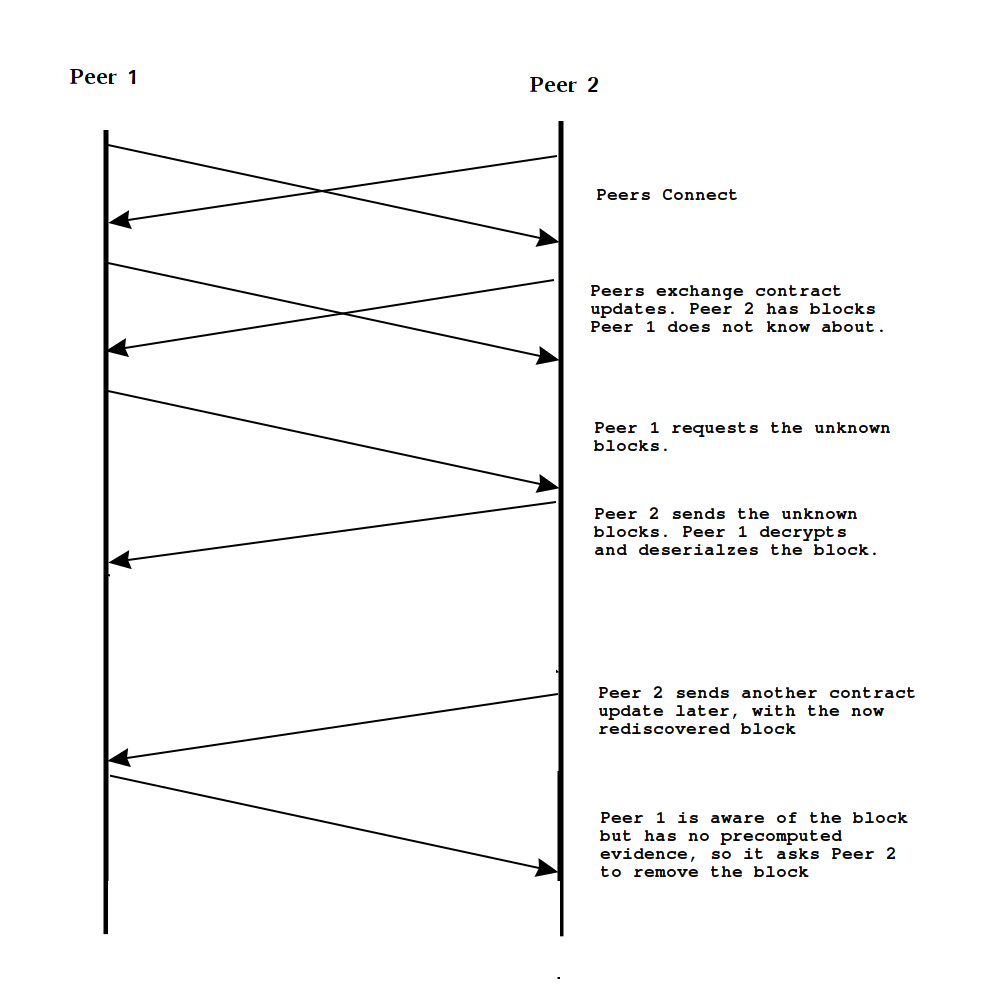
\includegraphics[width=0.8\textwidth]{lost-block}
 \caption{Lost Block Communication Example}
 \label{fig:lost-block}
\end{figure*}

If the PCM's appraisal by the peer was poor, losing all of the peers blocks may trigger contract termination, losing all of those blocks which would be unfortunate. This possibility is explored in section \ref{sec:peerAppraisal}. This would need to happen at least three times for all copies of shards held by peers to be removed causing data loss. The system correctly punishes peers that constantly lose all peer blocks.

This mechanism can be seen at work in figure \ref{fig:lost-block}.

\subsection{Peer Appraisal} \label{sec:peerAppraisal}

Peer Appraisal is the persistent trust system that allows for peer discrimination, based around three core metrics:

\begin{itemize}
 \item Common Uptime
 \item PDP Check Success Rate
 \item Block Loss Rate
\end{itemize}

We employ tools from intelligent agents to avoid potential attacks and design a system that uses a social approach \citep{pinyol2013computational} to control the acts of agents.

We first conduct a survey to see the viability of using uptime as a metric by polling users regarding their computer uptime. We find that within social groups uptime is correlated (fig. \ref{fig:uptime-survey}) confirming the potential for using peers to share storage for backup.

By sending a contract update a peer confirms they are online and we expect a given number of PDPs during the same hour. Each peer is given an array that stores the probability of a successful PDP for all shards during that hour of the week\footnote{A space of time in which we expect to see repeatable usage patterns based on the results of the survey in fig \ref{fig:uptime-survey}}. When the hour is complete we add $n$ to completed hour of the week.

$$n = \frac{\mbox{PDP Checked Shards}}{\mbox{Expected Shards}}$$

We also record the ratio of incomplete\footnote{$n$ is less than $1.0$} and fully complete reports, heavily penalising peers for incomplete reports as this indicates deceit. In addition we store a ratio of blocks lost vs. those that lasted their entire expected lifetime (two weeks).

We calculate peer appraisal with the following formula:

$$\mbox{rating} = H * R * L$$

where $H$ is the percentage of the time the peer was online at the same time the PCM, $R$ is the report completion ratio and $L$ is the block loss ratio. This produces a value that indicates the probability that the user will be online and able to pass PDP checks for all held shards, with a penalty for losing blocks.

\begin{figure}[h]
 \centering
 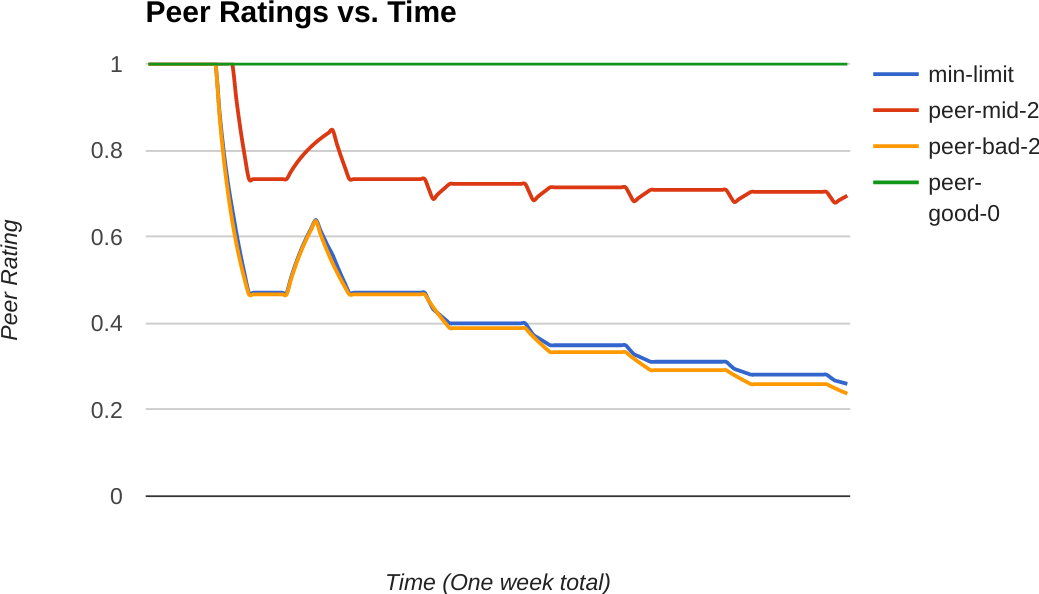
\includegraphics[width=0.7\textwidth]{peer-appraisal}
 \caption{Peer Appraisal Demonstration}
 \label{fig:peer-appraisal}
\end{figure}

If a peer rating is less than $\mu - \sigma$ we drop the peer as a contract, where $\sigma$ and $\mu$ indicates the standard deviation and mean respectively.

This system was simulated in unit testing, asserting that the peer appraisal correctly punishes peers that fail to deliver PDPs, have incompatible uptime or lose blocks.

We show a visual demonstration of the peer appraisal system in figure \ref{fig:peer-appraisal}. We configured the host generating these ratings to have a standard uptime taken from the uptime survey (\ref{fig:uptime-survey}). The good peer simulates a server with 100\% uptime and with no bad behaviour. The mid peer is online less than the host but during fairly similar times. The bad peer is only online for small parts of the weekend.

We also display the minimum rating to remain contracted as \code{min-limit} demonstrating that the bad peers would lose their contracts if there were two bad peers, two mid peers and one good peer present.

The rating mechanism is performing exactly as expected. A myriad of test cases using peers with different characteristics are tested numerically through automated unit tests ensuring the mechanism works correctly. We include a test to simulate what would happen if a peer contracted for four weeks suddenly loses all our data and assert that we would still remain contracted, and return the blocks.

Using \cite{josang2009challenges}'s nine potential attacks on reputation and trust systems described in section \ref{sec:tar} we ensure that the system is resilient to attacks.

A lot of attacks are countered by relying solely on image, instead of both image and reputation. Peers cannot use playbook, discrimination, collusion and Sybil attacks techniques. 

Peers are harshly punished for low-quality actions so a playbook attack is ineffective. Trust is instantaneous so it would be difficult to exploit reputation lag. A peer can re-enter the swarm with different credentials, but it would take a long time to regain reputation. Finally there are no easy actions the peer can perform that let them gain reputation.

As bad peers are shunned they will not have access to public PEX entries in high-performing peers, grouping poorly performing peer groups together, which is ideal.




\section{Networking}

The networking module is responsible for finding peers and providing a way to communicate with them. We first discuss authentication and account creation, followed by how we ensure peers can connect behind a NAT gateway, peers communication and how peers are able to locate each other. We end with the peer management strategy. 

\subsection{Authentication}

SSL is used for communication in Membrane. As the system is decentralised we cannot rely on a certificate authority for authentication, relying on a SHA-256 hash of the RSA public key, provided with the certificate on connection. This hash becomes the account for the peer.

If a peer is able to establish a secure connection with the provided certificate, we are certain the peer also holds the private key. \citep{menezes1996handbook} It is computationally infeasible to find the private key using only the public key, so we are guaranteed it is the same peer.

The probability that two peers will generate the same RSA key is small enough that it can be ignored. On first application launch we generate the RSA public key, private key and X.509 certificate, placing it in the Membrane config folder. Future application launches search this folder and load them into the application.

It is important that users store these credentials in a safe place. We prominently display this in the usage instructions, and in the future we plan to implement a utility to encrypt transfer the authentication information to a removable storage medium.

\subsection{Peer Connection}

We can expect Membrane peers to be behind a NAT gateway, grouping all internal IPs as one external IP. A host needs to use a NAT Traversal technique to map an external port to one of it's internal ports. A NAT gateway will typically block connections to unmapped ports. In section \ref{sec:p2pconn} we discussed four solutions, two of which we attempt. UPnP port forwarding \citep{boucadair2013universal} and TCP Hole Punching \citep{wing2010traversal}.

We use a UPnP communication library in Java for port forwarding. First we broadcast a UPnP request for potential gateways on the network. If a response is received we use UPnP to request a port forward for five minutes. If this request fails we try the next port up for a maximum of 20 attempts. In practice this has proven a large enough number to locate an available port. We then ask the gateway what the external IP is. A refresh is performed every 180 seconds to ensure the port forwarding entry never expires. A lifetime of five minutes is used to ensure the port forward stops after a reasonable time.

We attempt TCP Hole Punching but find that Vert.x, the chosen network communication library does not provide a way to both listen and send messages out of the same port. If users find that UPnP is insufficient we will investigate using the underlying communication library Netty to regain the required control.

In testing we discovered that as only one of the peers required port forwarding to generate a connection it is sufficient within the Membrane proof-of-concept.

\subsection{Peer Exchange (PEX)}

In order to allow peers that constantly change IP address and port to find each other require a method of PEX as discussed in the literature review (\ref{sec:pex}). We need to build on the PEX system used in BitTorrent in order to locate previously contracted peers in the swarm.

We introduce the concept of a \emph{PEX Advertisement}, \emph{PEX Request} and \emph{PEX Response}. Using these three messages we allow peers to locate each other within the swarm, without exposing information about peers that do no want their information public.

\subsubsection{PEX Advertisement}

Each peer periodically sends a PEX Advertisement with the following fields to all connected peers:

\begin{itemize}
 \item IP Address
 \item Port
 \item Time Stamp
 \item \code{isPublic} Flag
 \item Signature
\end{itemize}

On receipt the peer verifies the signature and checks for other entries from the same peer within its PEX Ledger, an evicting store of Peer PEX information. If this PEX advertisement was created after the latest entry it has, the update replaces the previous entry. To ensure this system is not broken by time stamps set in the future, these are automatically dropped. By default the ledger stores 300 PEX entries in the ledger, expiring them in FIFO order if full. The Ledger is persisted to disk periodically.

To sign the advertisement an RSA Signature, which can be imagined as a HMAC where the private key is used to generate a hash and the public key (contained in the X.509 certificate) is used to verify the signature against the message. The entire contents of the message (except the signature) is signed.

If a connection to the Peer is required the PEX IP address and port can be dialled to attempt a connection.

\subsubsection{PEX Request}

In the event that connection to a peer is lost, and both peers have changed address, PEX Requests can be used to attempt to find the location of the peer. A PEX request is sent to currently connected peers, asking for the most recent PEX Advertisement in their PEX ledger for the peer. The request must contain the peer id, which as established, is a sha-256 hash of their public RSA key.

The chance of guessing the key for an existing peer is sufficiently infeasible, that knowing the peer ID for the peer means the Membrane instance requesting the information has either connected to the peer before, or has heard about them at some point in time.

If there exists a PEX Advertisement Entry for the requested peer in the PEX Ledger of the peer that received the request, this is sent back in the PEX response as a PEX Advertisement.

As PEX Advertisements are signed using the original peers private key, we can be certain that the PEX response originated from the peer and was not forged. \citep{li1993remark} The time stamp in the advertisement prevents the peer sending old PEX Advertisement. The certificate of any contracted peer is persisted by Membrane to check for this signature. Therefore the PEX Advertisement can be reliably treated as if it came from the peer it describes.

\begin{figure*}
 \centering
 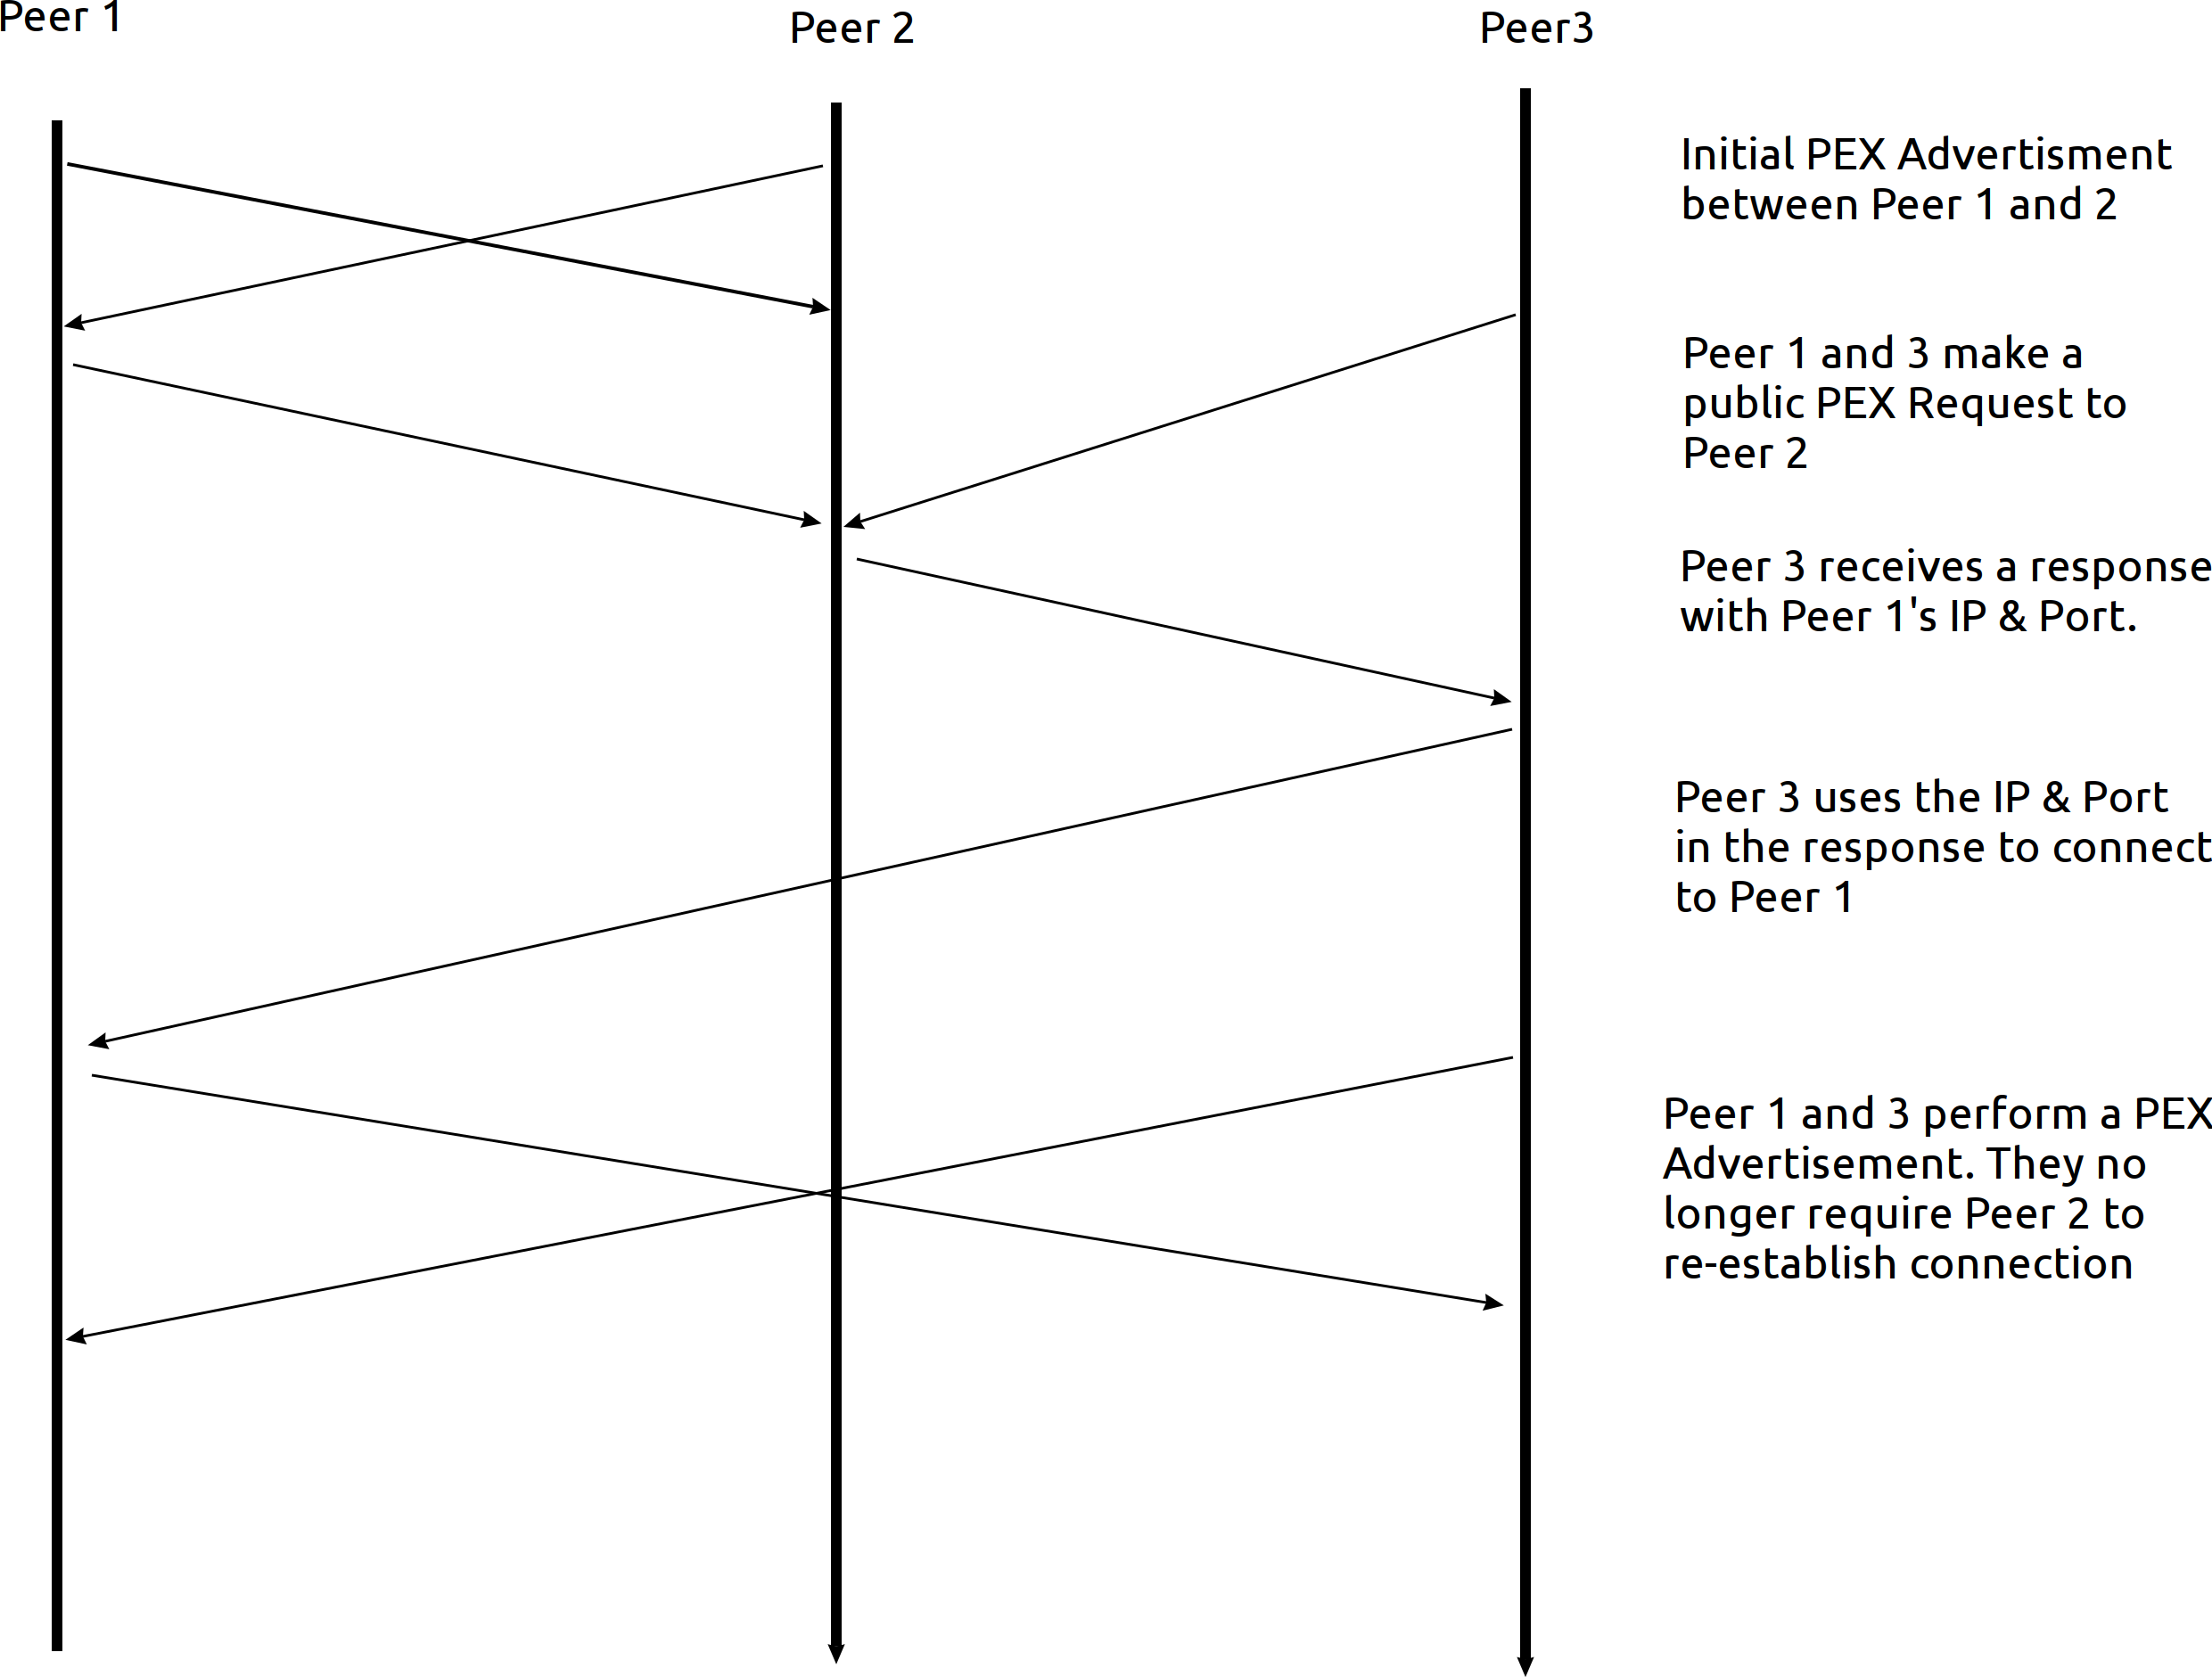
\includegraphics[width=0.8\textwidth]{pex-new-peer}
 \caption{PEX New Peer Discovery Example}
 \label{fig:pex-new-peer}
\end{figure*}

This mechanism is demonstrated in figure \ref{fig:pex-new-peer}. Two peers (1 and 3) attempt to relocate each other by using Peer 2.

\subsubsection{Public PEX Entries}

This mechanism is further extended to support public PEX entries. A PEX Request can also request fifty\footnote{Decided upon through observing the PEX mechanism in BitTorrent. \citep{vuze2010vuze}} public PEX entries. These are sent back without signature or peer ID information and are meant as an untrusted mechanism for attempting to establish peer connections.

These are stored in a second non-persisted temporary ledger and is a mechanism for discovering new peers. When peer A requests peer B for public PEX entries, peer B searches all entries in their real PEX Ledger, only selecting those entries less than 15 minutes old with the \code{isPublic} flag toggled.

We prevent amplified denial of service attacks\footnote{In which an attacker could send a IP to multiple peers, causing them all to fire connection requests at the peer} in two ways:

\begin{itemize}
 \item For an entry to be sent from a peer it must be in the real PEX ledge. This requires a signature, which requires RSA credentials, which requires work done by the generating peer to create the credentials.
 \item Only one entry per IP can exist in a public ledger. So at most one request is sent by each peer every few minutes from each IP.
\end{itemize}

If a peer is looking for new peers to connect, it can allow peers with unknown X.509 certificates to connect to it via SSL, and begin sending public PEX updates.

\subsubsection{Tracker}

A tracker is a peer found at a static IP, only running the networking module of Membrane and unable to form contracts with other peers. Is it a last resort mechanism for Membrane peers if they are unable to find other contracted peers or looking for more peers to contract. The PEX mechanism functions in exactly the same way.

The domain name of all available trackers and their user IDs is hard coded in all Membrane instances. A user may run a Membrane tracker, but as it cannot establish contracts it will quickly lose appraisal and be uncontracted.

Using a tracker has the disadvantage of giving Membrane a centralised target for attackers to take down. We mitigate this by introducing a collection of trackers the peer can connect to, all using domain names so they can be replaced if required.

\subsubsection{Summary}

The described system allows for peers to locate each other and discover new potential peers, fulfilling the requirements for PEX within Membrane. The ability for peer discovery demonstrated in figure \ref{fig:pex-new-peer} is unit tested and proven to work.

\subsection{Communication}

As established in the literature review (\ref{sec:comm}) we design an ontology for communication using the FIPA based agent communication language (ACL).

\subsubsection{Agent Communication Language}

The FIPA ACL specification based on the Speech Act theory \citep{labrou1999agent} comprises of:

\begin{itemize}
 \item A Communicative Act (or performative)
 \item An ACL Message Structure
 \item An Associated Ontology or Protocol
\end{itemize}

We choose to adapt the FIPA specification for use in Membrane replacing the standard performatives (CAs) with an implicit INFORM performative. This is a change from the performative based approach suggested in the literature review (\ref{sec:comm}) as we decide the benefits of creating a stateless protocol with no replies\footnote{As per the recommendation of \citep{google2017api}'s API guide}, saving client memory and decrease in programming complexity far outweighs the benefits of the message having redundant information describing the content.

Because of the extensiblity requirement, we have designed the message API such that performatives are completely compatible with current messages, they would simply be ignored by earlier versions.

We opt to use the following fields from the FIPA ACL specification \citep{fipa2002fipa}:

\begin{enumerate}
 \item sender - Peer id of the sender
 \item receiver - Peer id of the receiver
 \item conversation-id - Unique message id for every message. This rolls around to $0$ when $2^{64}-1$ is reached. (For Debugging Only)
 \item in-reply-to - The message id can be included. $-1$ indicates an empty field. (For Debugging Only)
 \item content - The content of the message
 \item protocol - Indicates the version number of Membrane for parsing
\end{enumerate}

We find this layout holds all the information required for handling messages. The \code{in-reply-to} field is \emph{only} used for a PING-PONG message exchange, where we send a PING and wait for the PONG to arrive to test connectivity.

\subsubsection{Protocol Design}

A protocol for both \emph{Block Storage} and \emph{Peer Exchange} messages is required. We discussed ontologies in section (\ref{sec:ontology}), but find the chosen contract technique does not require an ontology as it just relies on values rather than domain knowledge to make decisions.

We therefore follow the API design guide's suggestions for formatting data to provide content for the described ACL using object oriented techniques to structure data.

There are nine messages that need to be sent:

\begin{itemize}
 \item PING (For Debugging Only)
 \item PONG (For Debugging Only)
 \item Contract Update
 \item Evidence Request (Block Instruction)
 \item Evidence Response
 \item PEX Advertisement
 \item PEX Query
 \item PEX Response
 \item Data Block
\end{itemize}

Using the style guide suggests using base64 encoding byte arrays used for transferring blocks and salts described in RFC4648 \citep{josefsson2006base16}. It encodes each six bits of data as a byte to turn all bits into ASCII, causing a $\frac{4}{3}$ expansion in data size. This allows the data to be transferred a string within the ACL specified with expensive data expansion.

To improve on this we can chose a more efficient encoding such as \emph{basE91} \citep{joachim2015base91} or transfer data without packaging it in the ACL. While developing the proof-of-concept it was useful to transfer the data in base64 as it was easy to compare by eye, one of the main reasons it is suggested in \cite{google2017api}'s API style guide.

\subsection{Gatekeeper}

The gatekeeper is the section of the networking module is responsible for dialling and receiving connections from peers. It takes the maximum number of allowed connections, and whether it should aim to connect to uncontracted peers, and ensures only desirable peers connect. We include the relevant code in listing \ref{lst:peerPop}.

During a periodic sweep the Gatekeeper performs peer population maintenance, first sending PEX Requests, using the following rules:

\begin{itemize}
 \item Only send if more connections are required to fulfil the contract target requested.
 \item Only send if there are also more connections that can be established without going over the maximum connection count.
 \item If the gatekeeper is searching for new public peers modify the above PEX Request to also request public peers.
 \item Send a PEX Request asking for connection info to all contracted peers is sent to all connected peers.
 \item Do not wait for a response. The gatekeeper will react to PEX information if it arrives separately.
\end{itemize}

A PEX Advertisement is then sent to all peers with the external IP address and port collected from the UPnP port forwarding. The PEX Advertisement is public if searching for new peers and more contracted peers are required.

Any redundant peers\footnote{Those not contracted and not a tracker} are disconnected if the maximum connection count is surpassed.

Finally the trackers are dialled if the speed at which the gateway is finding new peers is too slow. It expects to connect to all contracted peers in 200 minutes. This is an estimated number that can later be tuned during testing with a full active Membrane network.

This maintenance procedure is sufficient to provide the PCM with new peers up to the requested maximum, while refraining to connect to the main trackers if unnecessary, satisfying the requirements for the Network Module.

\subsection{Summary}

The components described connect together to form a distributed backup program that can store data with other peers in exchange for storing their data as required.

We discussed the journey of a file from initial detection using file change notifications. Local storage using a hierarchical structure to store shards. Packaging into blocks using FIFO and knapsack for deployment with peers and ended with the module responsible for establishing connections to peers using a custom peer exchange and authentication system. We now discuss the interfaces developed for user interaction.

\chapter{User Interfaces}

In order to select folders for backup and recover files users require a user interface. As discussed in during analysis (\ref{sec:commonfeatures}) both a CLI and GUI are required. In the following chapter we delve into the building and design of the interfaces showing examples of usage.

\section{CLI}

A Command Line Interface (CLI) is a means of interacting with a computer program by issuing commands to the program in the form of successive lines of text. The program which handles the interface is commonly called a shell.

The CLI is less widely used by casual computer users who favour graphical user interfaces, typically being preferred by advanced users as they provide a more concise and powerful means of controlling applications or the operating system and allow for easier scripting.

A CLI typically requires less resources than a GUI, it is more expert friendly, easier to develop and easier to build alongside the main application as a result. On the other hand it does have a very steep learning curve, and is unsuitable for beginners.

As we are targetting more advanced users (\ref{txt:adv-users}) for the earlier versions of Membrane we make the CLI the main method of interaction.

\subsection{Commands}

Within the Unix based systems targeted for early versions of Membrane the following pattern is common for commands in Bash\footnote{Bourne again shell, a commonly used shell on Unix based systems.} \citep{gnu2016man}:

\begin{displayquote}
 \code{prompt command param1 param2 ... paramN}
\end{displayquote}

\code{prompt} is provided by the shell to give context to the command, the \code{command} targets the script or command to be executed, and \code{param} are optional parameters that tell the script or application what to execute.

We model the CLI of membrane after Git, taking inspiration from the years of evolution it has had. We require the following commands for Membrane: \code{status}, \code{files}, \code{peers}, \code{history}, \code{recover}, \code{storage}, \code{network}, \code{contracts}, \code{monitored-folders}, \code{monitored-files}, \code{watch-add}, \code{watching}, \code{watch-remove}.

An example command is shown below.

\begin{displayquote}
 \scriptsize
 \code{dominic@expiravit:\~\$ membrane status} \\
 \code{Status:         NORMAL} \\
 \code{Host:           expiravit:13200} \\
 \code{Version:        1.0.0-alpha.6} \\
 \code{Uptime:         02:13:49}
\end{displayquote}

This command structure is easy to learn as it will be familiar to most users and has been proven to work.

\subsection{Usability}

It is important to make CLI use as easy as possible. Three methods assist CLI users.

During first use users can use the command \code{membrane -h} or \code{membrane --help} for a complete manual on how to use the membrane CLI. If a user uses a command incorrectly or is unsure on a specific command they can use the \code{-h} flag to be given specific command usage instructions. At any point the \code{-v} flag can be used for verbose output, letting the user debug issues if anything does not work.

\begin{displayquote}
 \scriptsize
 \code{dominic@expiravit:\~\$ membrane history -h} \\
 \code{Usage: membrane history <file>}
\end{displayquote}

Helpful error messages are also provided to help the user debug issues. There is both CLI and daemon error checking, with error messages being as helpful as possible, providing examples and telling the user exactly why the command did not work.

\begin{displayquote}
 \scriptsize
 \code{dominic@expiravit:\~\$ membrane recover /tmp/f1.txt file2.txt} \\ \\
 \code{You must specify the full filePath.} \\
 \code{Example: /tmp/dir1/file.txt} \\
 \code{You provided: file2.txt}
\end{displayquote}

Finally we add tab completion to the CLI, a common feature of shells that allows the user to press a completion key\footnote{Typically Tab.} to show all the available options or complete the command if there is only one option remaining. This makes CLI usage both faster and more intuitive.

\subsection{Installation}

Although Membrane is available as a \code{jar} archive containing the daemon code and as a executable CLI, we provide both a \code{.deb} and \code{.rpm} package for ease of use. These contain install and uninstall scripts that place all of the files in sensible locations and setup features such as tab completion.

These also place soft links to the executables and scripts in the user's \code{\$PATH} which allows users to specify the name of the program instead of the full directory for the executables.

The install scripts also set the daemon up with \code{systemd}, a widely used init system \citep{saunders2015systemd} used to bootstrap the user environment and manage all processes, ensuring they are always in the requested state\footnote{Running in the case of Membrane}.

This allows Membrane users to easily manage the daemon and interact with it immediately after installation using tools they are familiar with.

\subsection{Summary}

The Membrane CLI maintains all of the advantages of a CLI. It is lightweight and available in a small 5MB package compared to the 56MB GUI. It requires a lot less resources to run and although only appropriate for advanced users, that is also the target user group for the Membrane proof-of-concept.

We offset the steep CLI learning curve by providing and using tools familiar to frequent CLI users, allowing them to learn commands as easily as possible. An example interaction with Membrane can be seen in listing \ref{lst:cli-status}.

\section{GUI}

A Graphical User Interfaces (GUI) allows users to interact with applications through icons and visual indicators. They were first introduced to reduce the learning curve associated with a CLI \citep{linfo2004gui} making it easier for new users to use applications.

The most common combination of elements in a GUI is: windows, icons, menus and pointers referred to as WIMP. \citep{van1997post} The GUI has become a standard in human computer interaction (HCI) and has influenced the workflow of most computer users.

We propose a GUI for monitoring in section \ref{sec:gui-req} to compete with other available backup solutions throughout the prototyping stage and plan to expand the GUI for general interaction as Membrane grows in the future. This section will discuss the choice of GUI framework, followed by usability decisions taken that influenced the design, ending with a demonstration of the interface.

\subsection{Technology Choice} \label{sec:gui-technology-choice}

The choice of GUI technology can drastically effect the feeling of the final product. We compare the three competing frameworks JavaFX, Qt and Electron used in cross platform GUI development.

JavaFX is a platform for GUI development within Java, first included with Java 8. It is made to replace Java Swing, promising a more consistent API and easy MVC pattern support. JavaFX unfortunately lacks traction resulting in less support in the real world seen in figure \ref{fig:gui-trends}, where the predecessor Swing and alternative Qt remain in the lead.

\begin{figure}[h]
 \centering
 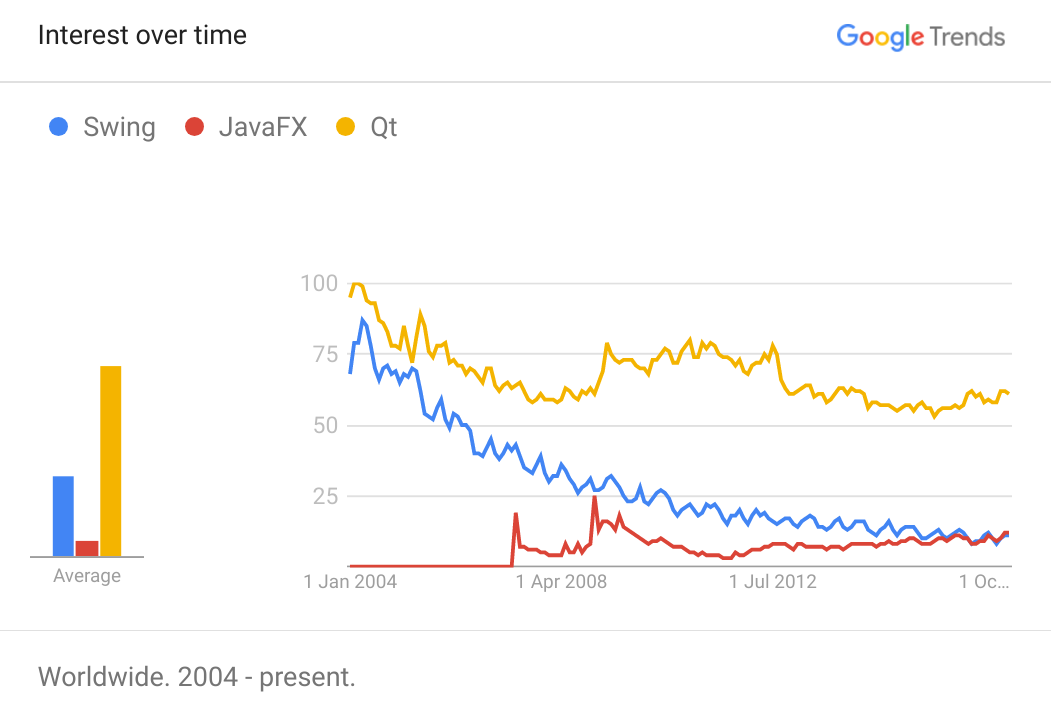
\includegraphics[width=0.5\textwidth]{gui-trends}
 \caption{GUI Framework Usage Trends (\url{trends.google.co.uk})}
 \label{fig:gui-trends}
\end{figure}

Qt is a CLI and GUI development framework for native feeling applications. It uses C++ with several extensions for signal handling. Several popular applications such as Autodesk Maya and VirtualBox \citep*{oracle2017logging, autodesk2017qt} make use of Qt. The benefits of Qt include the massive community and good professional documentation. \citep{slant2017qtelectron}

Electron is a much newer framework developed by Github. It uses Node.js for back-end and Chromium, the basis of the Chrome web browser for the front-end. It forms the basis of notable software such as Github's Atom and Microsoft Visual Studio Code \citep{james2015vselectron}. The community is very enthusiastic and active with hundreds of guides available and a solid API. Electron has the downside of being very heavy, using up a lot of memory unless developed with extreme care. Unfortunately we cannot find usage trends for Electron in figure \ref{fig:gui-trends}.

We opt for Electron for the Membrane GUI. It provides the best combination of ease of development and large community, with most of the support queries also being answered by in-browser web developers.

Although one of the requirements is for low-resource usage, this is the GUI rather than the main daemon so we do not have the same resource usage concerns.

\subsection{Usability Research}

In order to make the Membrane GUI as informative to the user as possible we look into Human Computer Interaction (HCI), specifically display designs which are typically designed to help with the perception and monitoring of relevant system variables, the exact goal of the Membrane GUI.

\cite{wickens1998introduction} describes thirteen principles split into four categories: perceptual, mental model, attention and memory principles. We look at each of these plan to design Membrane accordingly, while bearing in mind that we are designing Membrane with a minimum feature set \citep{blank2010mfs} and if the project gains traction the GUI can be improved in the future.

Principles that can be satisfied in the allocated time are met while those that are beyond the scope of the research are saved for further development. We still maintain the extensiblity requirement, ensuring that desirable features can be created in the future.

Legibility, top-down processing, information access cost and consistency are prioritised. We ensure all of the data is clear and cannot be misinterpreted, by presenting all the information in a clear listing in the centre of the application.

The information displayed is also split according to category so the user can easily find it and is not faced with unexpected and unnecessary information while using the application screens, adhering to the top-down processing principle.

We keep information access cost low, by ensuring every part of the application can be reached in one click and the user is always aware where they are in the application by clearly highlighted sections.

Finally we ensure application consistency by retaining static window decoration throughout the application. As the core sections of the application never change the user is always able to get to where they need.

Redundancy gain and pictorial realism are out of scope of the GUI. Instead of simply displaying information as text, for example storage space, a bar could be shown, indicating current usage, target usage and maximum usage, becoming more and more red as usage reaches the maximum.

This would help with user interaction, however, it is more important to get user feedback on Membrane as a whole instead of building the GUI to perfection and then finding that users do not like certain aspects of the daemon that would require a GUI redesign. 

We have have created an interface that is difficult to misinterpret and allows for simpler monitoring that the CLI.

\begin{figure*}
 \centering
 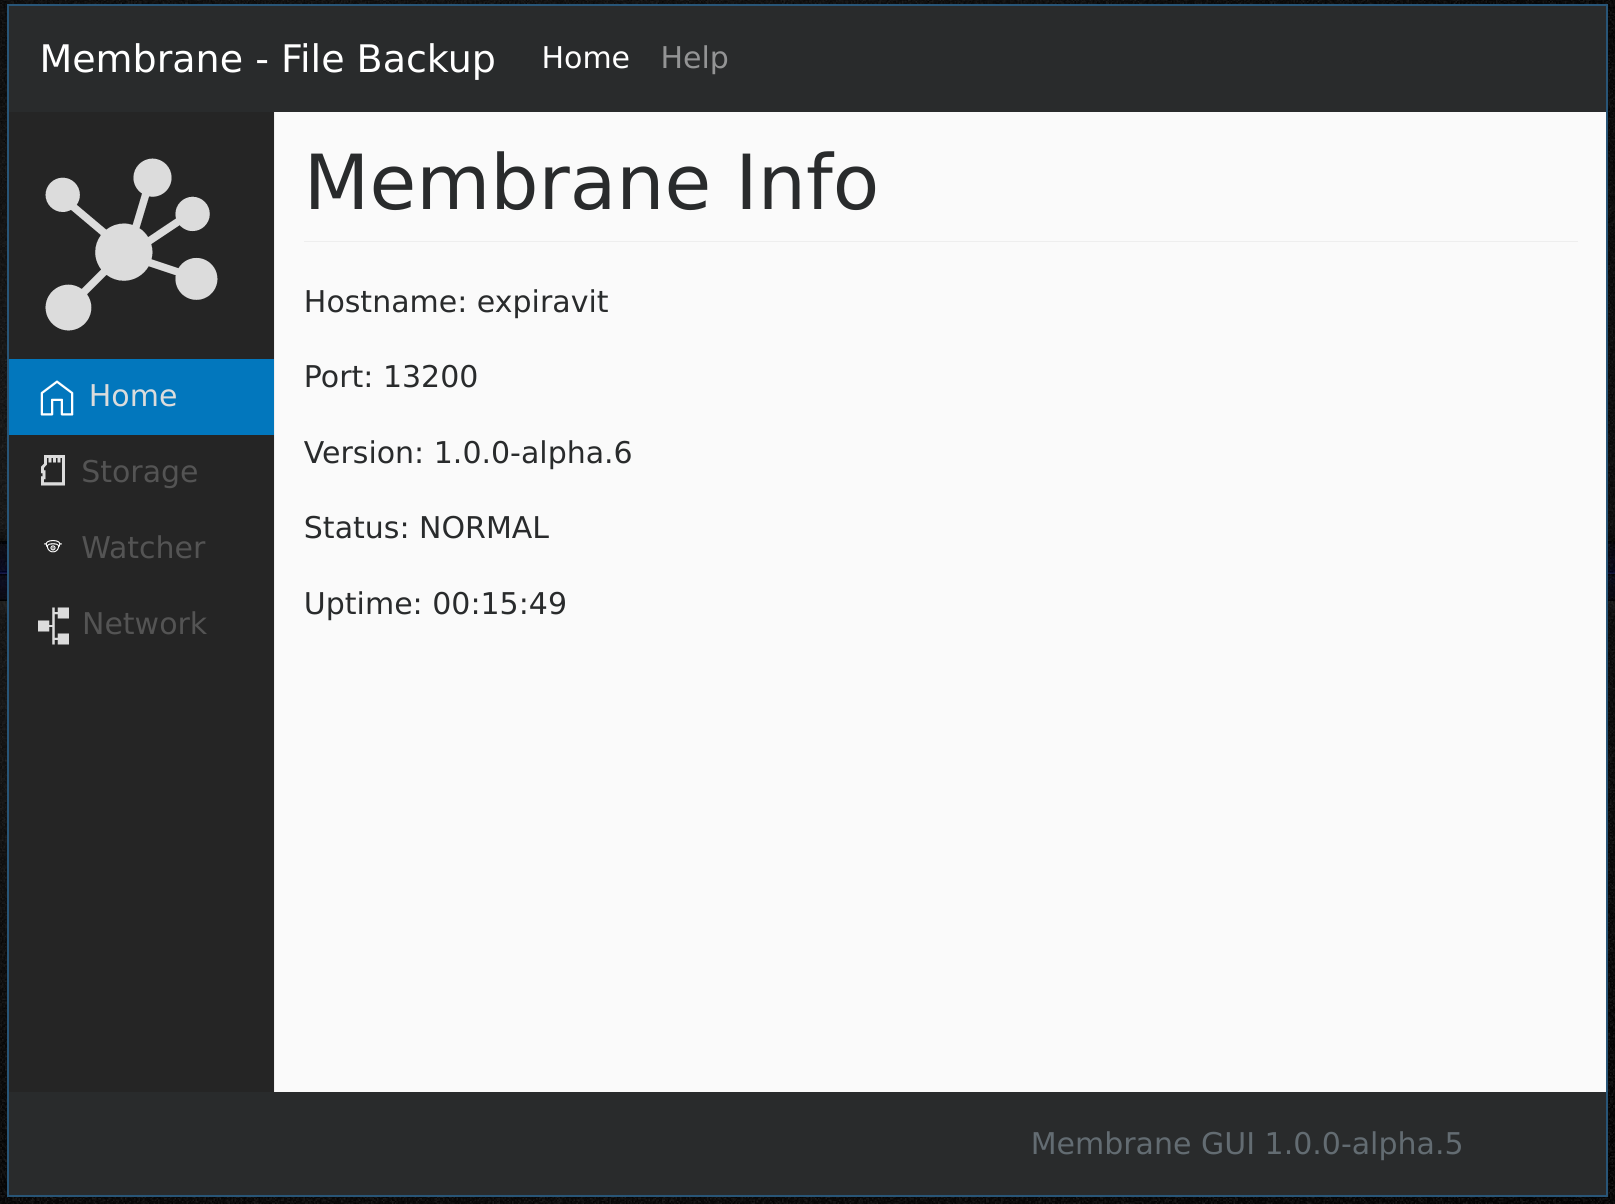
\includegraphics[width=\textwidth]{gui-main}
 \caption{GUI Main Screen}
 \label{fig:gui-main}
\end{figure*}

\subsection{Development}

Within Electron we built a simple web page that can display all of the required information. We make use of the popular front-end framework Bootstrap, developed by Twitter and Angular 2, a TypeScript based front-end web platform created by Google and a community of open source developers.

The main competitor against Angular, React.js was decided against as both frameworks offer very similar features and the developers creating the GUI were familiar with Angular, so we are unaffected by the higher learning curve of Angular \citep{house2016ng2react} and retain the use of TypeScript, which provides type correctness along with all of the other benefits discussed in section \ref{sec:typescript}.

The choice of Angular forces the MVC pattern to be used in the GUI architecture, splitting the application into services which hold the model and components which control the view. Angular connects these in the background controlling their interaction as the controller.

NPM is used for dependency management allowing packages to be automatically updated when required, automated packaging scripts and portability across multiple developments environments, fulfilling the role of Gradle in the JavaScript ecosystem.

\subsection{Design}

We now describe the design of the interface, which is split into four main sections. The home screen (fig. \ref{fig:gui-main}), storage (fig. \ref{fig:gui-storage}), watcher (fig. \ref{fig:gui-watcher}) and network screen (fig. \ref{fig:gui-network}). There is also a help screen (fig. \ref{fig:gui-help}) which contains a link to the main Github page with documentation and usage instructions.

\begin{figure*}
 \centering
 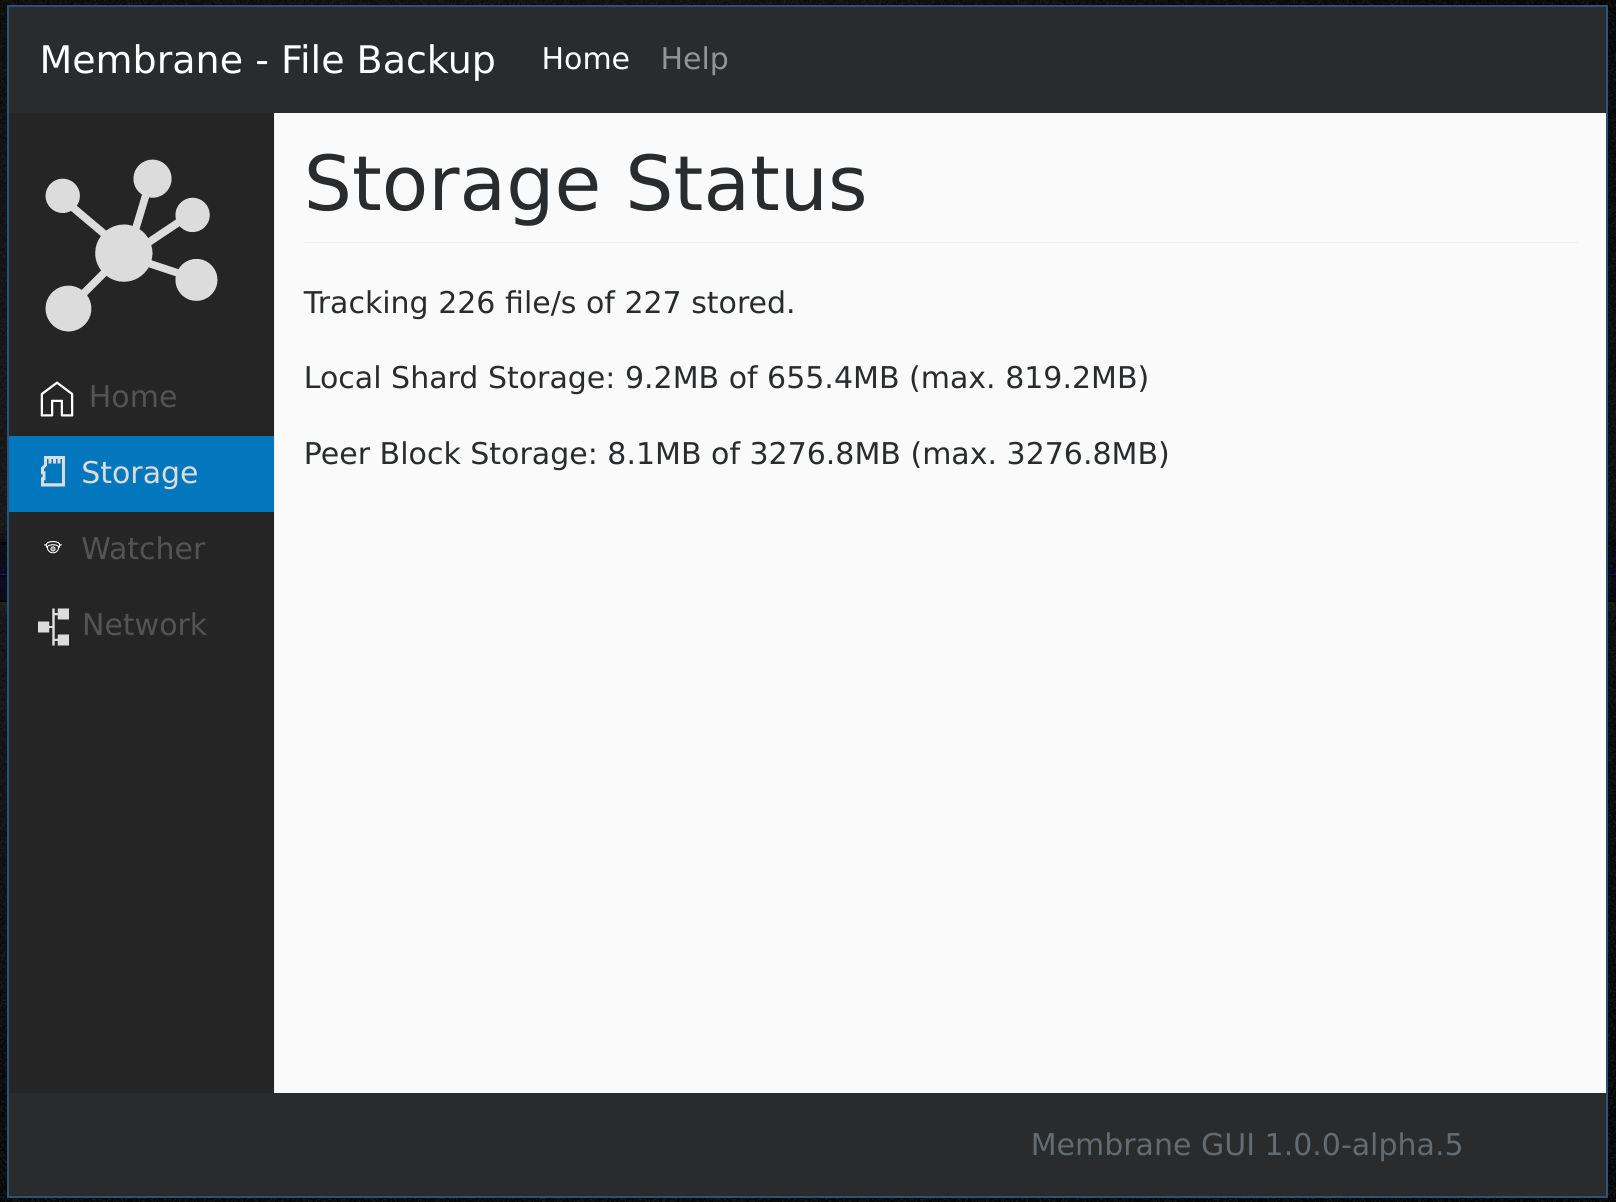
\includegraphics[width=\textwidth]{gui-storage}
 \caption{GUI Storage Screen}
 \label{fig:gui-storage}
\end{figure*}

The design is kept clean and simple with the information being the key focus of the interface. Any information that the user may want to observe, such as number of connected users, is included.

More complex information such as a listing of every file and folder monitored is excluded, as the user is expected to use the CLI for more complex interactions.

Navigation is assisted through using animations on elements that can be clicked, prompting the user to click on them, allowing for a more intuitive user experience.

\subsection{Installation}

The user can either choose to download a \code{tar.gz} archive containing just the GUI, A common Unix packaging technique, or the full Membrane \code{.rpm} or \code{.deb} packages which will automatically unpack the GUI into a sensible location and place it on the user path for simple access.

One of the downsides of Electron, is the size of the package. At 56MB after compression it is the largest part of Membrane, but this is a great trade-off for the ease of development provided by the framework and the quality of the resulting application.

\section{Configuration}

It is important to also mention the configuration file Membrane provides for user interaction. Users can manually add watch folders and much more advanced behaviour such as the number of connected users. This is currently only used for diagnosing problems, but is intended to be a way of tuning Membrane for advanced users in the future.

For many this a preferred form of interaction as users can use tools of their choice to modify and version control the configuration files, easily transferring options to new systems.

We ensure any interface manipulations are immediately persisted to the configuration file but require a restart to load configuration file changes, giving the user a chance to corrects mistakes without affecting any active instances of Membrane.

YAML a human readable serialisation language \citep{evans2009yaml} is used for the configuration file, making it as user friendly as possible. This is inspired by the configuration of Elasticsearch \citep{elastic2017config}, a popular distributed database.

By restricting some changes, such as the target number of contract and shard size to the config, we ensure that users will not accidentally modify key values during runtime. The fact the config can only be modified using root permissions also keeps new users away from dangerous changes that could adversely affect their backups.

\section{Conclusion}

We have provided two interfaces and three methods to allow users to configure Membrane. This fulfils the requirements (\ref{sec:commonfeatures}) and gives the users an variety of options for interaction.

With the daemon and interfaces complete Membrane is now complete and functional. It remains to test the functionality and ensure that users are able to use the application.

\chapter{Testing \& Evaluation}

It is crucial to test software before deployment, particularly if it is run by users where it cannot be monitored and handling user's personal data. We ensure it is impossible for Membrane to delete any files that it has not created or otherwise adversely affect the host system.

In this section we discuss three types of testing: unit, integration and usability outlining the importance and methodology in all three, trying to discover and address any problems discovered.

\section{Unit Testing}

Unit testing aims to test individual units of source code, to determine if they are fit for use and have expected inputs and outputs. \citep{huizinga2007automated} A unit is the smallest testable part of the application, ranging from an entire module to individual functions.

In order to isolate components of Membrane we make use of method stubs and mock objects \citep{osherove2015art} using Mockito, a library that uses reflection\footnote{A way of accessing encapsulated variables in objects.} for this. We also create temporary test objects such as the \code{EvictingContractManager}, in places where more complex mocking is required.

Test Driven Development (TDD) is used to scope modules while coding. We turn requirements into test cases breaking them down into constituent components that can co-exist. This technique uses the following development cycle \citep{beck2003test}:

\begin{enumerate}
 \item Create a test
 \item Run all tests and see if the new test fails.
 \item Write or modify code to ensure the test passes
 \item Refactor the code and move new code to where it logically belongs.
\end{enumerate}

By repeating this procedure the software grows without unnecessarily exceeding requirements. JUnit Jupiter is used as the testing framework. This integrates with Gradle into part of the project build, so any time code changes are made, tests are run to ensure code correctness.

\begin{figure*}[!ht]
 \centering
 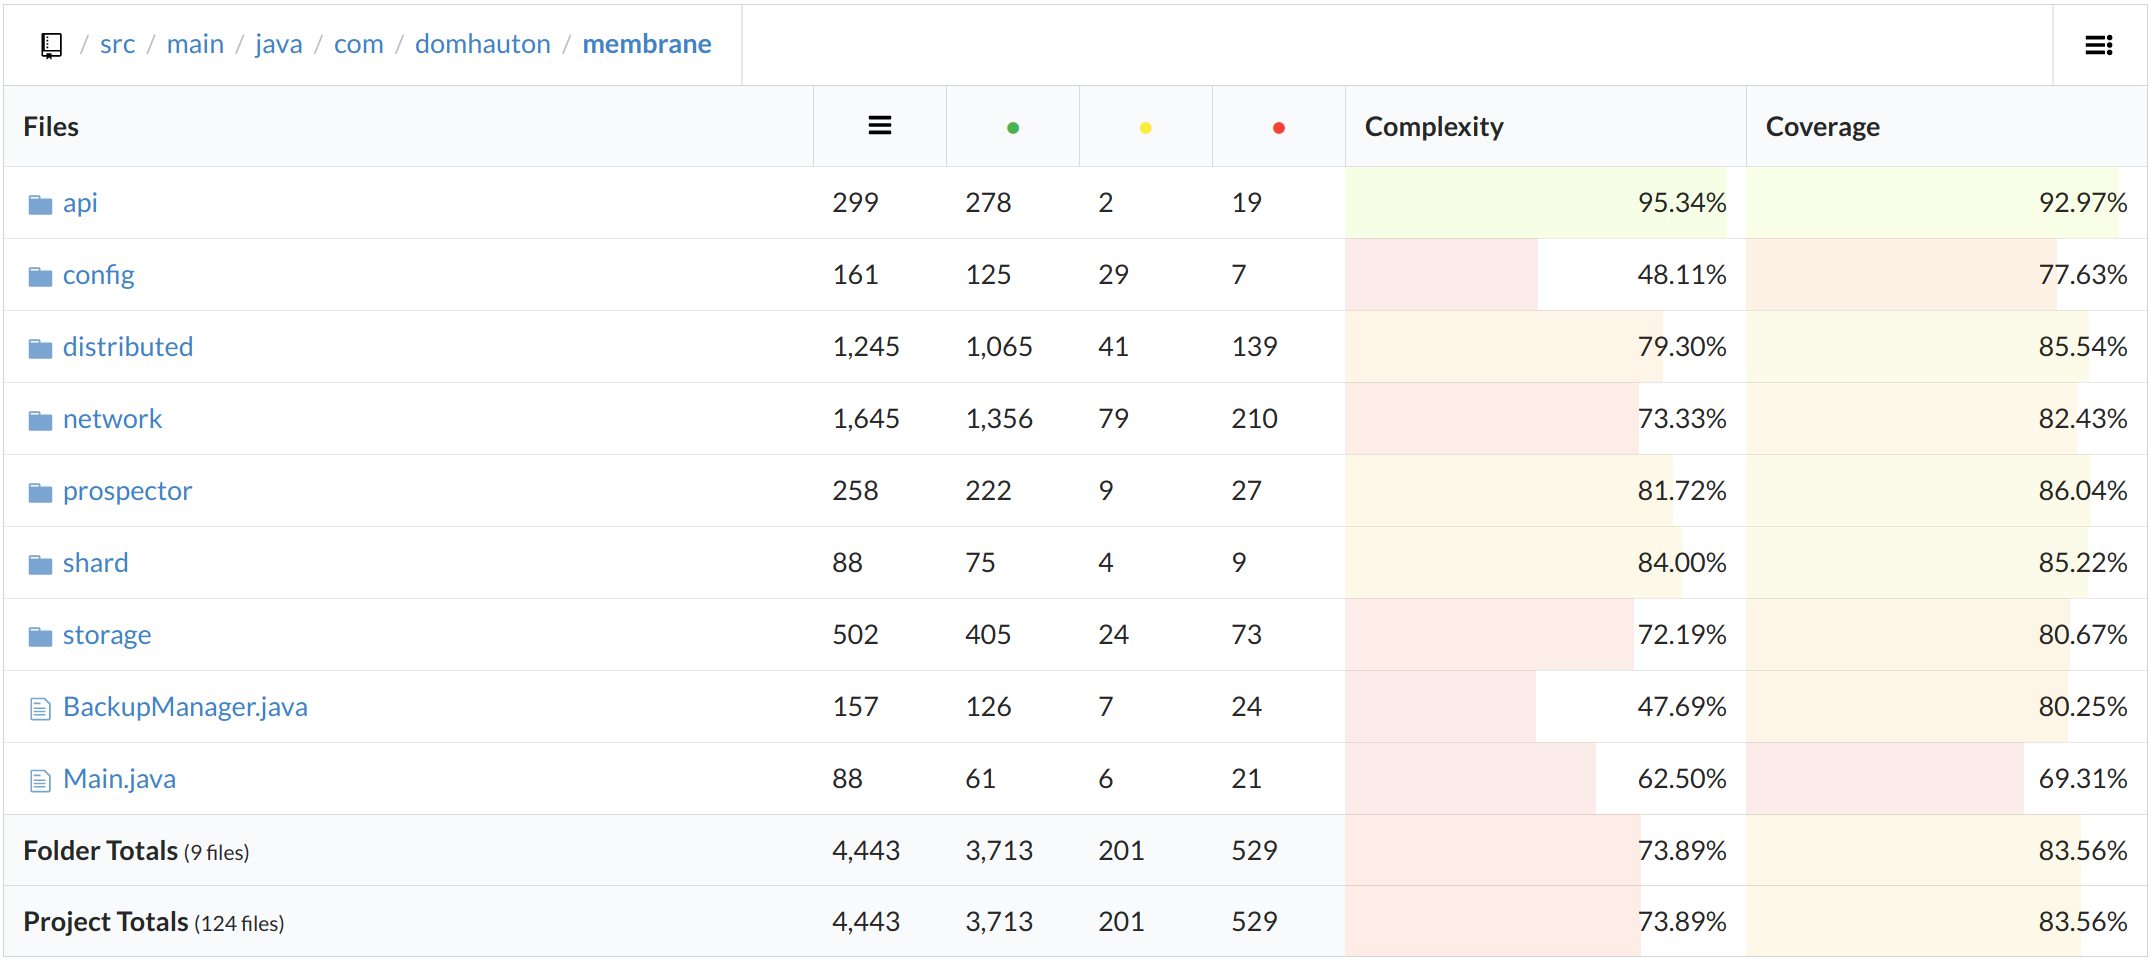
\includegraphics[width=\textwidth]{code-coverage}
 \caption{Membrane Code Coverage (\url{http://codecov.io/gh/domhauton/membraned})}
 \label{fig:code-coverage}
\end{figure*}

While designing unit tests it is important to prioritise areas of the program to test. Although it would be ideal to test every line of code sometimes this is impractical. An example of this is testing very niche situations such as, what would happen if the permissions on a config file changed mid-save. Although important to handle, creating an environment where this happens automatically is both time consuming and ultimately irrelevant compared to more important functionality.

Code coverage is a metric through which we can rate the unit test. This is a percentage of code lines that were executed during testing, a higher percentage usually indicating a lower number of unexpected bugs. \citep{miller1963systematic} More complicated coverage criteria such as branch coverage\footnote{Has every possible \code{if} statement been evaluated.} can also be used.

In Membrane we aim for 80\% line coverage and 70\% branch coverage. We measure this using VersionEye, a code coverage tool integrated into Github which tests code coverage on every commit and find that we achieve 83.20\% line and 73.74\% complexity coverage, varying slightly between modules as seen in figure \ref{fig:code-coverage} where green, yellow and red is full, partial and not covered line count respectively.

We ensure critical elements that could potentially cause problems for the user have 100\% coverage with every possible scenario considered.

\section{Integration Testing}

Integration testing combines all the software modules and tests them as a group. Its purpose is to verify both functional and non-functional requirements. The test cases focus less on individual object behaviour and more on the system as a whole.

There are a few integration test patterns to select from such a big-bang, bottom-up and top-down testing. \citep{binder2000testing} We opt for top-down testing which looks to approach testing from the main module, the \code{BackupManager} in Membrane, to all of the other sub-modules. One of the major advantages of this methodology is the ability to produce early skeletal program demonstrations, which was required during the ``demonstration of progress'' section of the project.

Throughout development we ensure the software is free of integration problems by using Continuous Integration (CI), a technique first proposed by \cite{booch1991object}. We adopt an evolution of the concept that advocates build servers that automatically build and test the project after every commit. 

Using TravisCI, a Github integration we test the code using both OpenJDK 8 and OpenJDK 9, a future version of Java ensuring we will have no trouble moving onto the more efficient JDK when it is fully released ensuring extensiblity. We are also able to automate deployment using TravisCI, assuring potential users who view the source code repository that the software is fully testing.

We finally ensure that all of the requirements have been met. This is done through a combination of unit and integration testing where appropriate. We find that all of requested functional requirements have been fulfilled and the software is ready for usability testing by the users.

\section{Usability Testing}

Usability Testing focuses on asserting software functionality with real users. It provides direct feedback on how the system will be used \citep{nielsen1994usability} allowing us to verify that the original goals of Membrane have been satisfied.

As we are not focusing on HCI testing, but rather the entirety of Membrane we choose hallway testing for our study. This is a quick and cheap method of testing that relies on asking a random selection of people to try Membrane. The only restriction in this methods is participants should not be too close to project, preventing bias.

\subsection{Methodology}

We use a slightly modified version of hallway testing, relying on remote testing and user feedback reflecting a true usage scenario. Using \cite{usajobs2014hallway}'s recommendations on successful hallway testing we design the test, slightly adapting their more physical testing scenario.

When deciding on a location we target user groups that enjoy technology and tinkering. This provides us with constructive feedback and is likely to have a higher overlap with people who use Unix-based operating systems compatible with the proof-of-concept version of Membrane.

We prepare the testing scenario by providing documentation and packaging the software. We provide both \code{.deb} and \code{.rpm} packages, covering a wide range of Linux users, as well as an online chat available at \url{https://gitter.im/mbrnd} for feedback and support. To make the test as authentic as possible we ask testers to simply visit the Membrane homepage (\url{http://mbrn.io}) and try to install the software. The markdown documentation the testers were presented with is also available in listing \ref{lst:readme}.

The full test specification that testers had to follow is available in the appendix (\ref{lst:mbrntst}). We run through the test in person with two testers first, to ensure the test plan works without issue. The volunteer is rewarded through a charity donation on their behalf and we take care to be mindful of the tester's time, by only requesting testers to perform one task that validates the project's main goals: a simple installation and the ability to backup files and recover them from the peer swarm after data loss. We hope the users are able to achieve this without external assistance.

At the end of the test we simply ask testers for written summary on their thoughts of using Membrane and completing the task, using the given feedback to assess the success of the project.

\subsection{Results}

The usability testing was conducted with five participants and the raw results are available in listing \ref{lst:mbrntestresult}. Overall the test was a success. Membrane was successfully installed on the participant's systems. With the instructions provided testers were able to successfully backup the requested files. When simulating a full system loss, Membrane was able to recover and reconstruct requested files.

The themes of the feedback are as follows:

\begin{itemize}
 \item Installation was short and simple. It did not cause any problems\footnote{One reported issue was caused because of incorrect RPM packaging, where the target system was unable to interpret \code{\#!/usr/bin/env bash} correctly at the start of scripts}.
 \item The concept of adding a watch folder did not cause issues.
 \item Copying authentication information out of Membrane needs some work but was achievable for all testers.
 \item Testers were surprised the GUI could only offer monitoring, despite this always being the intention.
 \item Recovery was always successful.
\end{itemize}

The feedback is very encouraging, demonstrating that the core logic of Membrane works although the interfaces could be improved. It is important to also consider the limitations of this study. 

The test was performed over a very short time span, so the trust mechanism could not be fully tested. As there were limited number of users online during testing\footnote{the maximum reaching four} it is difficult to fully assess the behaviour of the application when in a swarm of hundreds of users. But there is no inherent advantage or disadvantage to using a smaller swarm and it is promising that four of our five testers were able to use the distributed backup portion of Membrane with no issues.

One of our testers was unable to connect to peers. After a thorough investigation we find the subject was installing Membrane on a AWS hosted virtual server. The underlying hypervisor\footnote{An operating system with multiple embedded virtual operating systems.} of the virtual machine was interfering with the SSL handshake between two peers during connection, closing the connection mid-handshake. Debugging using Wireshark, a network protocol analyser that offers deep packet inspection gave no details as to the root of the issue.

The usability testing showcases that the components of Membrane work, and tell us where improvements need to be made during further development to increase adoption.

\section{Summary}

Throughout testing we have used well established techniques with modern tooling to prove with certainty that Membrane works and is capable of achieving all of the original requirements found during analysis (\ref{sec:requirements}).

We ensure it is impossible for Membrane to cause damage on a user's system and observe that all of the use-cases have been satisfied through unit, integration and usability testing.

With the Membrane tested we have a system ready for deployment to real users, barring a few patches requested by testers.

\chapter{Conclusion}

Throughout the project we studied, designed and built a marriage of distributed storage and backup technology. The problem was decomposed and researched ending in the creation of the distributed backup platform, Membrane.

In the conclusion we ruminate on the project, delving into the process and limitations, and planning the future development of the platform.

\section{Discussion}

We began the project by setting out the goal for Membrane:

\begin{displayquote}
 \emph{Allow users to easily backup and recover the contents of folders on their computer without needing to pay for a subscription-based service.}
\end{displayquote}

The project is designed to question the backup industry and explore the viability of a peer-based system that allows for file recovery without the need of a centralised system. We created a proof-of-concept, harnessing the cheap high-speed internet and redundant storage that many computer users have access to.

We structured Membrane into five distinct modules and list any challenges anticipated in the development process. These guided the literature review, from which we drew inspiration for the design.

\subsection{Literature Review}

Reflecting on the literature review, we find that although we were able to find solutions to all of the problems expected, in practice some of the ideas in literature are difficult or impractical to use.

An example of this is the reasoning system, which was made much simpler than the literature suggested it would need to be. This led to some of original research being redacted as we found more practical ways to implement aspects of the system.

Another example is ontology development which offers great flexibility and is powerful tool for communicating agents, but when agents have a single service and resource they can exchange information using simple protocols was easier to build and debug.

We also find that technologies researched that are presented as superior in literature fall short in practice due to limitations of tools, especially when faced with time constraints and working at a higher level of abstraction.

This manifested in the NAT Translation solution, in which we used the seemingly inferior  UPnP technique which requires support in the NAT gateway, but is much better documented and supported in Java than TCP hole punching. 

On balance despite the modifications required to the literature review during building we find that it is an invaluable tool for helping shape the project. It is however more helpful to treat it as an iterative tool that can grow with the project.

\subsection{Analysis}

After the literature review we proceed to the analysis, where we planned the design and structure of Membrane before starting development. We first questioned potential users on desired features. An insightful way to gather requirements, followed by a look at existing options.

Reflecting on the initial user poll, it would have been useful to discuss the final requirements with the polled users. Although all key requested requirements were fulfilled we find that the GUI was a far more desirable feature than first shown by polls and expected by almost all testers. In future projects we will go back with the completed requirements to the users after the initial poll giving them the opportunity to provide feedback at this early stage.

Looking at features of existing solutions, specifically looking at how they differ proved an extremely valuable way of scoping Membrane. Many of the desirable features discovered during the user survey were reiterated during the common feature analysis.

We discussed the concerns about requirements while creating them, aiming to make them brief and concise without formal dependencies. These proved perfect for the task with no misinterpretation. It is important to note in this case that requirement engineering and application development were fulfilled by the same person so small details may have been implicit, however, we postulate that with good communication the same details of requirements could be used within a development team.

The use cases presented proved the least helpful tool during analysis, requiring frequent modification as the software evolved. In retrospect use-cases should have been created after the software architecture was planned and the skeleton of the code was created, during which most of the modifications had to occurred. This would retain the benefits of ensuring all requirements were met and the ability to create integration tests around use-cases, while eliminating time required to keep them up-to-date.

Designing the architecture and selecting appropriate technology is required for any software project. Carefully assessing the technologies available saved time during implementation. We found the chosen N-Tier architecture good for testing and development allowing for simultaneous development of multiple sections and the ability to mock whole layers when required.

Separating the interfaces from the daemon also proved beneficial. The RESTful communication between components was well documented and easy to debug as suggested by literature.

\subsection{System Components}

\subsubsection{Monitoring}

The file system monitoring implementation covers all of the original software requirements, giving Membrane the ability to watch requested folders on the local file system, while adding new watch folders while running as efficiently as possible given the research performed. There are some points of expansion available, that would help processing speed and usability.

Firstly using a faster CRC32 checksum to check the file contents has not changed would allow for both more efficient operation and rsync style shard deduplication. This would be far more powerful and desirable method of deduplication.

We also limit users to using wild-cards to define folders instead of full regular expressions, which could provide a more comprehensive way of specifying folders.

It is important to remember that these were not included in order to control the size of Membrane and expected development time. As long as methods of adding these features later can be implemented later, Membrane does not lose out and we can get feedback faster to work on features that users like most. This is an important part of software development, as poor scoping can lead to projects that are never released.

\subsubsection{Local Storage}

The local storage system implemented is adapted from those used by distributed databases, resulting in a robust and resilient system as required by the specification. The challenge of this was not initially anticipated and we have identified several improvements that could have been made during implementation.

The local shard storage system is extensible with cloud block storage systems provided by companies like AWS, anticipating for access time and encryption layer shims\footnote{An addition that would mean all shards can be encrypted for storage and decrypted during reads}.

This was an unnecessary step that made the shard storage interface more limited than required and added feature envy\footnote{Logic relating to shard storage being present in other areas.} to both the file ledger and shard distribution (where a second instance was used for peer block storage). Although this will become useful in future iterations, it diverges from the minimum feature set ideology that guided development.

The file history implementation suffered from distributed storage influences. The original implementation using a write-ahead commit log prioritised writing instead of reading the data, and introduced requirements for indexing\footnote{Creating a copy of data optimised for specific searches} to increase read speeds, resulting in multiple representations of the data that need to be kept in sync.

The retroactive fix resulted in a patchwork of additions and a re-write of the module is required, conveniently made easily possible due to detailed unit testing. All-in-all the current implementation in the proof-of-concept does work, is stable and satisfies all expected requirements. Due to the modular nature of Membrane, the module could be swapped out with ease not affecting the majority of the code.

Overall the local shard storage system is a success, albeit with some cleanup required if new open-source developers were brought in to help with development.

The REST API development proved simple and was hugely successful. The ability to debug RESTful calls using tools such as curl\footnote{A Bash CLI tool to make HTTP requests} resulted in very fast development. The only downside encountered during development, was the requirement for a fixed listening port, meaning only one instance of the application could be run at a time. Outside of development testing this should never be required.

\subsubsection{Shard Distribution}

We come to the shard distribution module of Membrane, which focuses mostly on resource allocation and trust from multi-agent systems. This module required the most testing and was the most experimental section of the project, implementing a new heuristic based trust system and requiring meticulous testing to ensure the system works as expected.

The final system was able to correctly match appropriate storage agents and generate contracts with them. When we began development we aimed for a very complex negotiation system, prompted by MAS literature studied. Although the system should have worked in theory it also became very complex and after some development was dropped in favour of a negotiation free system that offered better flexibility and was more appropriate for the challenge posed.

Negotiation works in literature but, it requires two-way communication, which dramatically increases complexity and requires stateful messages. The networking layer does have support for stateful messages that wait for a response but it is easier for both debugging and construction to make the system fully stateless.

The constructed mechanism never requires a response to messages, keeping any state out of communication instead giving permission to peers and expecting permission back. It makes the response beneficial to the peer, prompting it. This system does not rely on timeouts or complex search required for negotiation keeping resource usage to a minimum with no downsides.

Another major benefit of the implemented system, is contracts scale with relationships, naturally making contract violations have less of an impact on desirable peers with lots of shared blocks and better peers being more likely to be chosen store more of our blocks.

Looking critically at the system it does fall short in two places. We cannot be sure the  offered space is real, meaning we might temporarily store blocks for peers that will never offer anything in return. This is the price for not having to wait until both peers have a block for upload and could be patched if this is abused.

The second flaw is that new peers have a high rating to begin with, so the required appraisal could be inflated if there an influx of new bad peers. We hope that with the target of 100 peers these spikes cannot have a significant impact on well established peers. A bad peer will also almost instantly start losing rating so this is slightly mitigated.

A final benefit of the distribution system is that peers are incentivised to report and send blocks to the PCM, removing the need for a DHT to map files in the swarm again reducing complexity.

\subsubsection{Networking}

The goal of the networking module was to provide secure connections to peer in the swarm. The PEX and authentication system built achieve exactly this.

Using Vert.x for communication means the system is entirely asynchronous. When a peer is dialled the rest of the system does not know if the dial is successful, a connection simply appears downstream after some time if successful, just as if the peer dialled reducing complexity by allowing for huge amounts of code reuse.

The PEX system was created from scratch, only drawing on some inspiration on BitTorrent. Again, the system achieves everything it was designed to do with no issues, allowing the re-location of old peers and discovery of new peers with minimal reliance on a centralised server.

Authentication was successfully completed using industry standard X.509 certificates and RSA encryption, guaranteed to be secure.

It is important to consider the limitations of the networking module.

We find one flaw of the PEX system. If we request information about another peer, the peer that received the request can now also request information about that peer, meaning the \code{isPublic} flag does not guarantee only contracted peers can find the peer. If this ever causes issues we could look into better systems, such as requiring the PEX Request to contain a signature of both their own and the peers ID signed by the peer being searched for. This would proving to anyone that the targeted peer has given the requesting peer permission to request their PEX information.

We also do not know how the PEX system scales with 100 users connected as planned. This would result in fifty PEX advertisements arriving per minute on average, which might need to be slowed down.

As RSA relies on the discrete prime factorisation problem it is not secure in a world with quantum computers which can use Shor's Algorithm to crack the encryption. We use a very long key at 4096-bits, however, this doesn't help against quantum computation. We are reassured by the fact that for the meantime, the most of the world uses RSA for authentication.

There is no implemented protection against denial of service attacks from peers sending large amounts of data. This would need to be implemented before Membrane can be fully deployed.

Finally, we use UPnP for listening across a NAT gateway. This does not work in every situation but we accept this as a limitation of the proof-of-concept.

\subsection{Testing}

Three types of testing were used in Membrane to demonstrate requirement satisfaction and prove the concept of distributed backup.

Unit testing was used during development to ensure individual software components worked as expected. We used JUnit and Mockito as the testing framework and used test driven development to ensure components were build correctly and to specification.

A major advantage of unit testing was how easy it was to modify components without concerns about the behaviour changing. This was taken advantage of during component refactoring, particularly while tuning the appraisal module ensuring correct peers were selected and values returned.

It was also useful while debugging issues, allowing very specific parts of the software to be run individually to observe behaviour.

Thorough logging also proved vital for debugging the system as a whole. When in \emph{trace} mode everything was logged, allowing developers to find unexpected actions and work backwards to see what caused them.

Integration testing was used to validate general system behaviour, using TDD to create module tests satisfying the requirements and use-cases.

With TDD integration testing it was difficult to predict the interfaces that needed to be tested for the module to work. During development it was common to add new methods for interaction and then have to modify the integration tests as a results.

On balance they provided the huge benefit of scoping the module so extra work was not done unnecessarily.

Usability testing was the most complex part of the testing as it required real participants. We used an adapted form of hallway testing to see if users would be able to install Membrane and accomplish a simple backup and recovery task. We gathered a lot of useful feedback, both finding bugs caused by running the software in new environments and generating feature requests for further improvements.

This was by far the most time-consuming testing but the feedback generated made the investment worthwhile. The main advantage of the hallway testing was how realistic the tests were, able to simulate how real users could potentially use Membrane on their systems.

As an improvement to the first round of hallway testing we will look to implement a method of providing feedback directly in test versions of the Membrane interfaces. This could automatically send logs to help test with large numbers of users. Despite only using five users for our testing, it took a few days to individually organise and test each run providing the test subjects with help if required. By letting people test the software in their own time and remotely provide feedback testing could be made much easier.

Overall the project is deemed a success. The system works is capable of the backup discussed in the introduction and with further development we believe it could potentially replace solutions like OneDrive which has notoriously bad Linux support for some users.

\section{Limitations}

The final software and project both have several limitations which need to be addressed. We shall expand on those mentioned during the discussion and include other limitations which we believe should be noted.

\subsection{Limitations of the System}

Distributed backup inherently has issues compared to using the cloud. The first is backup guarantee. Although Membrane does it's best to stop data loss, it can never guarantee that your data will be recoverable.

There is always a chance that all of the people holding your data will fail at the same as you. Cloud services have the same limitations as they need to store data on physical mediums too after all, but professional data centres will keep several backups on very stable platforms, with redundancy at every step.

With Membrane we can at best keep replicating data onto users who may unpredictably disappear without warning and do not have a mean time before failure (MTBF) metric like the hard drives which could be used to predict when peers will be lost.

Backup Size is also limited in distributed backup. The more secure the data should be the more redundant space we need with the requirement simply being a multiplier of the data we have sent out. With the system we have implemented there is no useful way to reduce this using peer block compression (as the blocks are encrypted) or using erasure coding as blocks are not guaranteed to be returned at the same time.

This limits Membrane's usefulness for full system backups, however, many cloud users only use the free storage provided with their account on sign up, typically around 10GB which is easily achievable for Membrane, only requiring 40GB of redundant space 40GB.

As shown during the initial survey users are concerned, and rightly so, about the resource usage of backup software. If we wish to provide PDP, a requirement within Membrane then users will be required to read and perform calculations on at least some of the data they have stored for others periodically. This will use bandwidth, CPU and disk and we can at most limit this.

An interesting idea would be to allow the addition of trusted friends who do not need to perform PDP for data, providing much more predictable uptime and reducing the requirement for as many copies.

The final limitation is the size of the swarm required for Membrane to become viable. We aim for each user to establish 100 contracts to be able to spread their data over a wide range of peers, reducing the impact of a peer disappearing. This will certainly not be the case during early Membrane development so we require significant interest before peek usability is reached and we can assess the efficiency of the system.

We will look at providing an option to backup to cloud block storage, eliminating most of the concerns described above, giving users the option to pay a small amount to use Membrane for both secure cloud backup and distributed backup as an extra redundancy and recovery feature.

\subsection{Limitations of the Study}

As discussed previously, during user testing the Membrane swarm was small. Our testing gives us no indication of the effects of large numbers of users using Membrane.

To fully test the implementation the bugs uncovered up during the initial study need to be addressed and a public beta would need to be started, hopefully bringing in large numbers of users for more comprehensive testing.

We can attempt to simulate a large number of peers but to get the desired feedback we require real users. We could then observe the effects of limited network bandwidth and latency on the solution.

In short, Membrane works in the lab, but the distributed nature means real-world performance could be much different.

\section{Further Work}

The software in it's current state is a proof-of-concept, demonstrating that distributed backup is indeed possible and the concepts behind it are sound. We look into the four main features users have demanded in both the initial survey and during hallway testing.

\subsection{USB Credential Store}

Throughout hallway testing, users reported that the method of extracting credentials from Membrane was clunky and very easy to do incorrectly. We propose a system that encrypts the credentials and launcher, placing them onto a USB stick along side a script for easy single command installation and restoration.

By automating the process we stop users ever needing to visit the root-owned folder that holds Membrane's backups, making the process much safer and simpler.

\subsection{GUI Improvements}

The GUI was another concern raised by testers. We plan to completely overhaul the GUI, converting it into the only mechanism required to interact with Membrane. This would help improve interaction with Membrane making it accessible to those that do not like interacting with applications over a CLI.

This would also alleviate usability problems discovered with the CLI, as it would become aimed solely for expert users who do not have access to the GUI, for example on a headless server.

\subsection{Cloud Integration}

As discussed in the limitations, cloud integration with commercial cloud services would offer a cheap way for users to backup and recover data eliminating most of the downsides of distributed storage.

We designed the shard storage to be replaceable with cloud block storage APIs, so users would simply need to provide their credentials to start backing up at \$0.005/GB/Month \citep{backblaze2017pricing} or other services. This is much cheaper than any plan offered by solutions like Dropbox or Google Drive.

It is important to note that block storage services offer free upload, extremely cheap storage but make money on download fees when users need to access data\footnote{\citep{backblaze2017pricing} charges \$0.02/GB for download, compared to \$0.005/GB/Month for storage.}.  

Membrane users would benefit from the cheap storage on block storage services such as Backblaze, without having to pay for download unless it is a last resort and Membrane cannot recover blocks that it backed up with peers, offering the best of both worlds.

\subsection{FUSE Mount}

The current method of accessing files requires a command per file version the user wishes to recover, which is only useful if the user wants a very specific file. Although we could allow for full folder recover in one command, FUSE offers a much better solution by allowing us to mount a virtual file system on the user's file system.

The user could select the time slice they wish to recover from using a slider on the GUI, and the FUSE mount would reflect the state of the system at that point in time, allowing the user could copy files out using familiar tools. Membrane would reconstruct files on the fly as the file system requested them.

\section{Summary}

Throughout the project we analysed, design and built the proof-of-concept for an amalgam of distributed storage and backup technology, demonstrating that it is indeed possible to create a system that fairly exchanges your data with peers, to provide backup, file versioning and recovery.

The four planning techniques used: scrum boards, Gantt charts, weekly supervisor meetings and weekly goals proved a highly effective way of ensuring the project stayed on track through the process. Problems were identified early and corrected immediately causing no issues.

We find that Membrane can provide all of the requirements set out during the specification, successfully testing the validity of the software using unit, integration and usability testing. Feedback gathered from system was mainly positive with concerns mostly revolving around the interface which can easily be improved now the concept is proven.

We also find the limitations of the concept: constraints on storage space dictated by the redundant space on the host machine, the possibility that all the peers holding a portion of data disappear when it is needed for recovery, periodic system resource usage for proving to peers you still hold their data and finally the need for a large group of users also using the service.

Overall the original goals of the project are satisfied. We successfully created a program that allows users to backup files and recover them from peers after data loss, with simple installation that does not require any expert knowledge.

With the four suggested extensions: a USB credential store, improvements to the GUI, integration with cloud block storage for emergency access and FUSE mount file retrieval Membrane becomes an excellent cheap backup tool.

\bibliography{dissertation}

\newpage

\chapter{Appendix}

\section{Software}

The source code is provided in three parts all located in different folders within the provided tar archive.

The use of an IDE is highly recommended while perusing code due to the size of the project, which contains roughly 22,000 lines of production and test code spread over roughly 300 files.

IDE config files for IntelliJ Idea 2017.1 (Daemon), Webstorm 2017.1 (GUI) and Gogland PREVIEW (CLI) are included with the source code.

The code is also available on Github. We recommend visiting \url{http://mbrn.io} to browse, checkout and install Membrane, however, all of the code is also available in the following states in the provided multi-part zip\footnote{The multi-part zip houses the aforementioned tar.}:

\begin{itemize}
 \item Source code - Copies of the code repositories hosted on Github
 \item Compiled code - Compiled versions of the source code that can be run immediately
 \item Packages - Software packages that can be installed using the README in the Appendix 
\end{itemize}

\subsection{Source Code}

Available in three folders containing different software parts. The instructions pull the freshest code available from the git repository. If you want to use the submitted code simply copy the folder from \code{membrane-code/source}.

\subsubsection{Daemon}

\begin{itemize}
 \item To run this code you must install Java 8 and Gradle.
 \item The software has been tested on Ubuntu 16.10 but should work on any Unix system.
 \item Run the following commands with a Network Connection
 \begin{enumerate}
  \item \code{git clone git@github.com:domhauton/membraned.git}
  \item \code{cd membraned}
  \item \code{./gradlew --refresh-dependencies clean check shadowJar -Dscan}
  \item \code{java -jar build/libs/membraned-1.0.0-alpha.7-all.jar -v}
 \end{enumerate}
 \item Gradle script will run unit tests and ensure membrane works on your system
 \item The final command runs the daemon in verbose mode.
\end{itemize}

\subsubsection{CLI}

\begin{itemize}
 \item To run this code you must install golang 1.8.
 \item The software has been tested on Ubuntu 16.10 but should work on any Unix system.
 \item Run the following commands
 \begin{enumerate}
  \item \code{git clone git@github.com:domhauton/membrane-cli.git}
  \item \code{cd membrane-cli/}
  \item \code{export GOPATH="\$(pwd)"}
  \item \code{go build -o bin/membrane src/domhauton.com/membranecli/membrane.go}
  \item \code{bin/membrane status}
 \end{enumerate}
 \item Run commands using \code{bin/membrane param1 param2}
 \item Instructions are found in the README (Listing \ref{lst:readme})
 \item Use \code{bin/membrane -h} for help
\end{itemize}

\subsubsection{GUI}

\begin{itemize}
 \item To run this code you must install nodejs.
 \item The software has been tested on Ubuntu 16.10 but should work on any Unix system.
 \item Run the following commands with a Network Connection
 \begin{enumerate}
  \item \code{sudo npm install typescript -g}
  \item \code{sudo npm install tslint -g}
  \item \code{sudo npm install electron -g}
  \item \code{sudo npm install electron-packager -g}
  
  \item \code{git clone git@github.com:domhauton/membrane-gui.git}
  \item \code{cd membrane-gui/src}
  \item \code{npm install}
  \item \code{node\_modules/electron/dist/electron main.js}
 \end{enumerate}
 \item The GUI should appear.
\end{itemize}

\subsection{Compiled Code}

Available in three folders containing different software parts. Instructions assume you are in \code{membrane-code/compiled}.

\subsubsection{Daemon}

\begin{itemize}
 \item To run this code you must install Java 8
 \item The software has been tested on Ubuntu 16.10 but should work on any Unix system.
 \item Run the following commands
 \begin{enumerate}
  \item \code{java -jar membraned/membraned-1.0.0-alpha.7-all.jar -v}
 \end{enumerate}
 \item The final command runs the daemon in verbose mode.
\end{itemize}

\subsubsection{CLI}

\begin{itemize}
 \item This code has no requirements.
 \item The software has been tested on Ubuntu 16.10 but should work on any Unix system.
 \item Run the following commands
 \begin{enumerate}
  \item \code{membrane-cli/membrane status}
 \end{enumerate}
 \item Run commands using \code{membrane-cli/membrane param1 param2}
 \item Instructions are found in the README (Listing \ref{lst:readme})
 \item Use \code{membrane-cli/membrane -h} for help
\end{itemize}

\subsubsection{GUI}

\begin{itemize}
 \item To run this code you must install nodejs.
 \item The software has been tested on Ubuntu 16.10 but should work on any Unix system.
 \item Run the following commands
 \begin{enumerate}
  \item \code{membrane-gui/membrane-gui/membrane-gui}
 \end{enumerate}
 \item The GUI should appear.
\end{itemize}

\subsection{Packaged Code}

Packages can be found in: \code{membrane-code/packages}.

Use the instructions found in the README (Listing \ref{lst:readme})

\section{Code Snippets}

\begin{lstlisting}[language=Java, caption=Garbage Collection Implementation, label=lst:fileGC]
  /**
   * Removes any shards not referenced in the catalogue from the storage.
   */
  long collectGarbage() {
    logger.info("Garbage collection - Start");
    Set<String> requiredShards = fileCatalogue.getReferencedShards();
    Set<String> garbageShards = shardStorage.listShardIds();
    garbageShards.removeAll(requiredShards);
    garbageShards.removeAll(tempProtectedShards);
    logger.info("Garbage collection - Found {} de-referenced shards", garbageShards.size());
    AtomicLong removedSize = new AtomicLong(0L);
    garbageShards.stream()
            .peek(x -> logger.info("Garbage collection - Removing shard: [{}]", x))
            .forEach(x -> {
              try {
                long fileSize = shardStorage.removeShard(x);
                removedSize.addAndGet(fileSize);
              } catch (ShardStorageException e) {
                // Ignore - It doesn't exist already
              }
            });
    logger.info("Garbage collection - Complete - Removed {}MB", ((float) removedSize.get()) / (1024 * 1024));
    return removedSize.get();
  }
\end{lstlisting}

\begin{lstlisting}[language=Java, caption=Storage Clamping Implementation, label=lst:storageClamping]
  public synchronized long clampStorageToSize(long bytes, Set<Path> trackedFolders) throws StorageManagerException {
    long currentStorageSize = getStorageSize();
    long spaceToRecover = currentStorageSize - bytes;
    logger.info("Space Recovery - Reducing storage to {}MB. Current size {}MB. Need to remove {}MB", ((float) bytes) / (1024 * 1024), ((float) currentStorageSize) / (1024 * 1024), ((float) Math.max(spaceToRecover, 0)) / (1024 * 1024));
    if (spaceToRecover > 0) {
      logger.info("Space Recovery - Collecting unnecessary shards.");
      spaceToRecover -= collectGarbage();
    }

    if (spaceToRecover > 0) {
      logger.info("Space Recovery - Finding un-tracked files.");
      Set<Path> notTrackedFiles = fileCatalogue.getCurrentFiles().stream()
              .filter(x -> !trackedFolders.contains(x.getParent()))
              .collect(Collectors.toSet());
      if (notTrackedFiles.size() > 0) {
        logger.info("Space Recovery - Removing {} un-tracked files.", notTrackedFiles.size());
        notTrackedFiles.forEach(x -> fileCatalogue.forgetFile(x));
        spaceToRecover -= cleanStorage(fileCatalogue.getOldestJournalEntryTime());
      } else {
        logger.info("Space Recovery - No un-tracked files found.", notTrackedFiles.size());
      }
    }

    if (spaceToRecover > 0) {
      logger.info("Space Recovery - Retiring older journal entries.");
      fileCatalogue.removeOldestJournalEntries((int) spaceToRecover);
      spaceToRecover -= cleanStorage(fileCatalogue.getOldestJournalEntryTime());
    }

    if (spaceToRecover > 0) {
      logger.warn("Space Recovery - Could not meet {}MB requirement. Excess is {}MB.", ((float) bytes) / (1024 * 1024), ((float) spaceToRecover) / (1024 * 1024));
    } else {
      logger.info("Space Recovery - Successful file size reduction. Reduced to {}MB.", ((float) (bytes + spaceToRecover)) / (1024 * 1024));
    }
    return spaceToRecover;
  }
\end{lstlisting}

\begin{lstlisting}[language=Java, caption=Knapsack Shard to Block Fitter, label=lst:shard2block]
  public static Set<String> calculateBestShards(String[] shardIds, int[] shardSizes, int blockSize) {
    boolean[][] retainShard = new boolean[shardSizes.length][blockSize + 1];
    int[][] tmpTable = new int[shardSizes.length + 1][blockSize + 1];

    for (int shardIdx = 1; shardIdx <= shardSizes.length; shardIdx++) {
      for (int size = 1; size <= blockSize; size++) {
        if (shardSizes[shardIdx-1] > size) {
          tmpTable[shardIdx][size] = tmpTable[shardIdx-1][size];
        } else {
          int keepShardSize = shardSizes[shardIdx-1] + tmpTable[shardIdx-1][size-shardSizes[shardIdx-1]];
          int ignoreShardSize = tmpTable[shardIdx-1][size];
          if (keepShardSize > ignoreShardSize) {
            retainShard[shardIdx-1][size] = true;
            tmpTable[shardIdx][size] = keepShardSize;
          } else {
            tmpTable[shardIdx][size] = ignoreShardSize;
          }
        }
      }
    }

    Set<String> selectedShards = new HashSet<>();
    for (int i = shardSizes.length-1; i >= 0; i--) {
      if (retainShard[i][blockSize]) {
        selectedShards.add(shardIds[i]);
        blockSize = blockSize - shardSizes[i];
      }
    }
    return selectedShards;
  }
\end{lstlisting}

\begin{lstlisting}[language=Java, caption=Peer Population Control, label=lst:peerPop]
  /**
   * Attempt to connect to new peers, spread PEX information and disconnect redundant peers.
   */
  void maintainPeerPopulation() {
    logger.info("Running peer maintenance.");
    Set<String> contractedPeers = contractManager.getContractedPeers();
    Set<String> connectedPeers = connectionManager.getAllConnectedPeerIds();
    Set<String> trackerPeers = trackerManager.getTrackerIds();

    // First attempt to connect to any peers with pre-established contracts
    connectToContractedPeers(contractedPeers, connectedPeers);


    // Check if new connections are required and have space
    int knownPeerCount = getKnownPeerCount(contractedPeers, connectedPeers, friendPeers, trackerPeers);
    int remainingConnectionCount = remainingConnections(knownPeerCount, maxConnections);
    int requiredConnections = requiredPeers(knownPeerCount, contractManager.getContractCountTarget());

    boolean requireMoreConnections = requiredConnections > 0;
    boolean haveRemainingConnections = remainingConnectionCount > 0;

    logger.info("{} more peer connections for contracts. {} to connect to more peers. Should {} connect to new public peers",
        requireMoreConnections ? "Require" : "Do not require",
        haveRemainingConnections ? "Able" : "Unable",
        searchForNewPublicPeers ? "" : "not");

    Collection<Peer> connectedPeerSet = connectionManager.getAllConnectedPeers();

    if (requireMoreConnections && haveRemainingConnections) {
      PexManager.requestPexInformation(connectedPeerSet, contractedPeers, searchForNewPublicPeers);
      if (searchForNewPublicPeers) {
        pexManager.connectToPublicPeersInPex(connectionManager, requiredConnections);
      }
    }

    boolean isPexUpdatePublic = searchForNewPublicPeers && requireMoreConnections;

    ExternalAddress externalAddress = portForwardingService.getExternalAddress();
    logger.debug("Sending external address {}:{}", externalAddress.getIpAddress(), externalAddress.getPort());
    PexManager.sendPexUpdate(externalAddress, connectedPeerSet, isPexUpdatePublic);

    // Disconnect from peers taking up useful connection slots

    if (remainingConnectionCount < 0) {
      logger.debug("Need to disconnect redundant peers. Too many connections.");
      disconnectRedundantPeers(-remainingConnectionCount, contractedPeers, connectedPeerSet);
    }

    // Connect to a tracker if struggling for peers.

    logger.info("Checking if tracker connection necessary.");
    int contractedPeerTarget = contractManager == null ? 0 : contractManager.getContractCountTarget();
    int connectedPeerCount = connectedPeerSet.size();
    int minutesFromStartup = Minutes.minutesBetween(startUpDateTime, DateTime.now()).getMinutes();
    boolean hasPexEntries = pexManager.getPexEntryCount() > 0;

    if (trackerManager.shouldConnectToTrackers(contractedPeerTarget, hasPexEntries, minutesFromStartup, connectedPeerCount)) {
      logger.debug("Connecting to tracker to assist locating more peers.");
      trackerManager.connectToTrackers(connectionManager, connectedPeers);
    } else {
      logger.info("Tracker connection not required.");
    }
  }
\end{lstlisting}

\section{Documents}

\begin{lstlisting}[language=RsT, caption=Membrane README (\url{http://mbrn.io}), label=lst:readme]
# Membrane Daemon

Membrane is a Distributed Backup System that swaps your storage space with other users in the Membrane swarm to backup your data.

Features
--------

- Both [GUI](https://github.com/domhauton/membrane-gui) and [CLI](https://github.com/domhauton/membrane-cli) interfaces
- File history ensures file versions are never removed until necessary.
- Log in from anywhere using your generated 4096-bit RSA key
- Twofish encryption ensuring strong security for data privacy.
- Deduplication reduces storage requirements for similar files.
- Prioritise backup to friends and family.

Installation
------------

- Download the 
[deb](https://github.com/domhauton/membraned/releases/download/1.0.0-alpha.7/
membrane-1.0.0-alpha.7.deb) or [rpm](https://github.com/domhauton/membraned/releases/download/1.0.0-alpha.7/
membrane-1.0.0.alpha.7.rpm) package
- Install using `dpkg -i /path/to/membrane-1.0.0-alpha.7.deb` or `rpm -i /path/to/membrane-1.0.0-alpha.7.rpm`
- Start the daemon using `sudo systemctl start membraned.service`
- Check status using `membrane status`
- Run GUI using `membrane-gui`
- Logs can be viewed using `journalctl -u membraned.service`
- Backup your credentials from `/root/.config/membrane/auth`
- To restore another account replace `/root/.config/membrane/auth` with your backed up credentials

Requirements
------------

- Java 8 or above
- Systemd (if using packages)

Usage
-----

- Use the GUI to monitor the membrane daemon `membrane-gui`
- To add watch folders to backup use `membrane watch-add <folder>`
- To check backed up files use `membrane files`
- To explore file history use `membrane history <file>`
- To recover file use `membrane recover <file> <target> <optional: date>`
- Use the `-h` flag at any point for command help

Support
-------

If you are having issues, please let us know.

We have a mailing list located at: support@mbrn.io

License
-------

The project is licensed under the MIT license.
\end{lstlisting}


\begin{lstlisting}[language=RsT, caption=Membrane API Documentation, label=lst:apiDocs]
API
---

The Rest API is available on port ``13200`` by default.

Available Calls include:

Status
~~~~~~

- **URL** : /
- **Method** : GET
- **Response Params** : {hostname: [string], startTime: [dateTime], port: [number], version: [string], status: [string], tagline: [string]}
- **Response Codes** : Success (200 OK), Unauthorized (403), Internal Error (500)

Network
~~~~~~~

- **URL** : /status/network
- **Method** : GET
- **Response Params** : {enabled : [bool], connectedPeers: [number], networkUID: [string], maxConnectionCount: [number], peerListeningPort: [number], upnpAddress: [string]}
- **Response Codes** : Success (200 OK), Unauthorized (403), Internal Error (500)

Storage
~~~~~~~

- **URL** : /status/storage
- **Method** : GET
- **Response Params** : {currentFiles: [string[]], referencedFiles: [string[]], localShardStorageSize: [number], targetLocalShardStorageSize: [number], maxLocalShardStorageSize: [number], peerBlockStorageSize: [number], targetPeerBlockStorageSize: [number], maxPeerBlockStorageSize: [number]}
- **Response Codes** : Success (200 OK), Unauthorized (403), Internal Error (500)

Watcher
~~~~~~~

- **URL** : /status/watcher
- **Method** : GET
- **Response Params** : {trackedFolders: [string[]], trackedFiles: [string[]]}
- **Response Codes** : Success (200 OK), Unauthorized (403), Internal Error (500)

Watch Folders
~~~~~~~~~~~~~

- **URL** : /status/watch_folder
- **Method** : GET
- **Response Params** : {watchFolders: [watchFolder[]]}
- **Response Codes** : Success (200 OK), Unauthorized (403), Internal Error (500)
- **Other** : watchFolder = {directory: [string], recursive: [bool]}

Contract
~~~~~~~~

- **URL** : /status/contract
- **Method** : GET
- **Response Params** : {contractManagerActive: [boolean], contractTarget: [number], contractedPeers: [string[]], undeployedShards: [string[]], partiallyDistributedShards: [string[]], fullyDistributedShards: [string[]]}
- **Response Codes** : Success (200 OK), Unauthorized (403), Internal Error (500)

Modify Watch Folder
~~~~~~~~~~~~~~~~~~~

- **URL** : /configure/watch_folder
- **Method** : POST
- **Request Params** : {type: [string (ADD|REMOVE)], watchFolder: [watchFolder]}
- **Response Codes** : Success (200 OK), Partial Fail (304), Invalid Request (400), Unauthorized (403), Internal Error (500)
- **Other** : watchFolder = {directory: [string], recursive: [bool]}


Request Storage Cleanup
~~~~~~~~~~~~~~~~~~~~~~~

- **URL** : /request/cleanup
- **Method** : POST
- **Response Codes** : Success (200 OK), Invalid Request (400), Unauthorized (403), Internal Error (500)


Reconstruct File
~~~~~~~~~~~~~~~~

- **URL** : /request/reconstruct
- **Method** : POST
- **Request Params** : {filepath: [string]}
- **Response Codes** : Success (200 OK), Partial Fail (304), Invalid Request (400), Unauthorized (403), Internal Error (500)


Request File History
~~~~~~~~~~~~~~~~~~~~

- **URL** : /request/history
- **Method** : POST
- **Request Params** : {filepath: [string], targetFilePath: [string], dateTimeMillis: [number]}
- **Response Params** : {filePath: [string], fileHistoryEntryList: [fileHistoryEntry[]]}
- **Response Codes** : Success (200 OK), Partial Fail (304), Invalid Request (400), Unauthorized (403), Internal Error (500)
- **Other** : fileHistoryEntry = {dateTime: [string], hashes: [string[]], size: [number], remove: [boolean]}
\end{lstlisting}

\begin{lstlisting}[language=RsT, caption=CLI Usage Example, label=lst:cli-status]
dominic@expiravit:/tmp/mbrn-test$ membrane 
contracts          history            monitored-folders  peers              status             watch-add          watch-remove
files              monitored-files    network            recover            storage            watching           


dominic@expiravit:/tmp/mbrn-test$ membrane status 
Status:         NORMAL
Host:           expiravit:13200
Version:        1.0.0-alpha.6
Uptime:         00:31:14


dominic@expiravit:/tmp/mbrn-test$ membrane storage 
226 current files stored.
227 total files.
Local Shard Storage. 9MB of 655MB used (max 819MB)
Peer Block Storage. 8MB of 3276MB used (max 3276MB)


dominic@expiravit:/tmp/mbrn-test$ membrane contracts 
Peers Contracted:       3 (max. 100)
Undeployed Shards:      0
Partially Deployed:     225
Fully Deployed:         0


dominic@expiravit:/tmp/mbrn-test$ membrane network 
User ID:        92d81c1cb271d4110a3fec62cdeb41e352a63f391421ca9316e36525806a0b9d
Peers:          2 (max. 100)
Peer Port:      14200
UPnP Address:   81.135.110.126:14217


dominic@expiravit:/tmp/mbrn-test$ membrane peers 
Contracted Peer(s):
        e71ef553a177fef4fb4af6fd555f486bf33b02e9224b9c2dd15ec1e4eea8caf9
        4df5387fc333612205b4715df6cb8e5160f20ac772fe15449bc394a90f98e7e2
        de9426306d4e1adca19dec07529e669b809239cbeab20e51f0c785479e73c0d2
\end{lstlisting}

\section{Tables}

\begin{table}[h!]
\centering
\label{tab:storageUsage}
\begin{tabular}{|l|l|l|l|l|}
\hline
       & Total File Size (MB) & Total Number of Blocks & Effective Block Size (MB) & Efficiency \\ \hline
User 1 & 4111                 & 176                    & 4400                      & 0.93       \\ \hline
User 2 & 8556                 & 387                    & 9375                      & 0.88       \\ \hline
User 3 & 758                  & 34                     & 850                       & 0.89       \\ \hline
\end{tabular}
\caption{Storage Usage vs. Actual File Size}
\end{table}

\section{Surveys}

\begin{lstlisting}[language=RsT, caption=Membrane Feature Survey, label=lst:mbrnsurvey]
 Question: What 5 features would you be looking for in a distributed backup system, that uses a network of peers to add resilience to your data?
   
 Response 1:
 - Make sure my data is safe
 - Should be easy to setup and not require my attention
 - Should avoid using too much of my network as I have limited data
 - Should not slow down my games
 - I would like a web interface like dropbox has 
  
 Response 2:
 - I don't want to have to care about it after setup
 - Should let me see old copies of my work
 - People storing my data shouldn't be able to see it
 - I want to be able to view the backups in a window
 - I need to be able to get my files back quickly if I delete them accidentally (like a recycle bin)
 
  
 Response 3:
 - I don't want to have to rely on the speed of peer's connections to recover files.
 - I want to be able to move my files from system to system, like onedrive does.
 - Don't use data when connected to a phone hotspot from my laptop
 - No-one can be able to see my files.
 - A way to recover files by just plugging a USB stick in.
 
  
 Response 4:
 - Strong encryption - something that, to the best of the knowledge in the community, has not been ``broken'' and would take even super computers and exorbitant amount of time to brute force
 - I use OneDrive to move files from my desktop to my laptop, this would need to be able to do the same.
 - I don't wat to ever have to think about the backup service unless I'm recovering files. Should be completely transparent to me.
 - The option to be able to use my own server for backup. I don't want to only rely on the network for backup.
 - A good syncing feature like OneDrive so what is in the backup is always up to date, with at least a OneDrive level of versioning or better (deleted files are recoverable but changes are not)
 
  
 Response 5:
 - The people storing my files cannot see them
 - Should be able to see old documents. If I make a change to something and want to go back to the previous version I should be able to.
 - I use Google Photos for image backups. A system that showed my a nice album of the images I backed up would be cool.
 - Transfer Files Between System
 - I want to be able to use this from a USB stick, plug it in and it immediatly starts backing up and recovering files.
 
  
 Response 6:
 - This needs to be able to work without my babysitting it, and cannot break!
 - It needs to use an unbreakable encryption for my files. I don't want any chance of someone seeing the data they are backing up for me. I also want to be sure I'm not backing up anything illegal for anyone else!
 - I need quick access to any files I backup. Otherwise this is useless.
 - This can't be a drain on my laptop battery. If I noticed my fans spin up on my laptop because of backup, I would immedialy uninstall it.
 - I sometimes use Google Drive to access my file from uni for example. It would be nice if I could do the same with this.
 
 
  Response 7:
 - I want to be able to just backup to my friends
 - No wait for file recovery
 - Should be able to see old file version, like in dropbox
 - Can't slow down my computer
 - I want to be able to add friends who I trust
  
  
 Response 8:
 - This cannot use too much of my laptop battery.
 - I use dropbox for file versioning sometimes, this needs to be able to do the same.
 - This needs to be able to run without me noticing it, just like dropbox.
 - It needs to be able to show my old versions of files. I also want to be able to share files I've backed up from other people's computers.
 - It wouldn't be a must by any stretch, but I think it would be nice to have 1 backup tool that handles everything.  As in, it does this cloud sync thing, but you can also plug in an external drive and it uses the same tech to fill it up, etc.
\end{lstlisting}

\begin{lstlisting}[language=RsT, caption=Membrane Hallway Test Guide, label=lst:mbrntst]
 Hallway Test Instructions for Testers
 =====================================
 
 This is a guide for Membrane testers.
 
 For every test complete a £5 charity donation will be made to http://www.extra-life.org/
 
 Goals
 -----
 
 Testing the usability of Membrane, ensuring it works as expected.
 
 Instructions
 ------------
 
 1. Visit http://mbrn.io and follow the installation instructions
 2. Ensure Membrane is running
 3. Checkout the membraned git repository into a folder in /tmp
 4. Add the folder you just checked out as a recursive watch folder to Membrane.
 5. Ensure the backup is successful and all shards have been exchanged with at least one other peer.
 6. Backup the Membrane credentials manually onto your machine.
 7. Uninstall Membrane.
 8. Delete the checked out git repository
 9. Delete `/root/.membrane` and `/root/.config/membrane` folders on your machine.
 
 10. Install Membrane and run it once to regenerate the config folders.
 11. Replace the new generated credentials with your old credentials and restart Membrane.
 12. Wait until Membrane displays recovered files.
 13. Recover `/tmp/membraned/README.md`
 
 Feedback and Support
 --------------------
 
 Please provide any observations and potential improvements in `gitter.im/mbrnd` or via chat with Dominic Hauton
\end{lstlisting}

\begin{lstlisting}[language=RsT, caption=Membrane Hallway Test Feedback, label=lst:mbrntestresult]
 Response 1:
 - Easy installation
 - Gui was okay for watching the backups but should be improved.
 - Fairly responsive, seemed to find people without any issues, wasn't able to fully backup the folders though.
 - Re-installation was a bit convoluted but it worked.
 - Was able to recover the requested file fairly quickly in the end. Nice!
  
 Response 2:
 - Was okay to install, but would be better with a real page
 - Wasn't able to connect to any hosts, but the local part of the backup worked.
 - I've sent you over logs as requested.
 - Was able to recover the files from the local copy, as you suggested.
 
 Response 3:
 - Was a bit fiddly to store the 'auth info'. It should be one file!
 - Fairly easy to add watch folders. It should fill in the directories for me too. Not just the commands.
 - Recovery was okay, but same as above, you have to be very precise with names while typing them in..
 - Overall it worked, obviously needs some love before release to the masses though.
  
 Response 4:
 - You should put sudo in the installation instruction, I was copy pasting and the command failed because of that.
 - I wasn't able to do anything through the gui. I had to use the command line, you should be able to set up the whole backup through the gui.
 - Had a few failed commands while using the command line. Help was okay though, you should consider a man page.
 - Recovery worked fairly quickly, neat.
 
 Response 5:
 - Had a bit of trouble installing using the rpm. Was able to diagnose issues over chat though.
 - Backup worked.
 - Recovery worked but should be able to do more over the gui.
\end{lstlisting}

\section{Use Cases} \label{sec:apdx-usecase}

\setlist{nolistsep}
\subsection{Add Watch Folder}
The expected behaviour of Membrane during a normal backup operation when a new folder is added. The computer owner is primary actor.

\subsubsection{Goal}

Store redundant copies of files on the system

\subsubsection{Steps}

\begin{enumerate}
 \item User adds folder for backup with files.
 \item Folder is persisted to the configuration file.
 \item New files in folder are detected.
 \item Files are sharded into equal chunks and sent to shard storage.
 \item The change is logged and saved in the file's history.
\end{enumerate}

\subsubsection{Extensions}
\begin{enumerate}
  \item Submitted folder does not exist:
	\begin{enumerate}
	  \item Accept entry and wait until it does.
	\end{enumerate}
  \item Cannot persist watch folder due to IO error
	\begin{enumerate}
	  \item Inform the user
	  \item Do not continue
	\end{enumerate}
  \item Shard storage full:
	\begin{enumerate}
	  \item Do not log the change in file history.
	  \item Shorten the history until soft limit is reached.
	  \item Retry submission later.
	\end{enumerate}
  \item Cannot log change in file history:
	\begin{enumerate}
	  \item Leave new shards.
	  \item Retry submission later.
	\end{enumerate}
\end{enumerate}


\subsubsection{Variations}
\begin{enumerate}
  \item Folder is file:
	\begin{enumerate}
	  \item continue and wait until file becomes a folder
	\end{enumerate}
  \item File present in multiple watch folders:
	\begin{enumerate}
	  \item De-duplicate file by sharding
	  \item log changes from both folders if path different
	\end{enumerate}
\end{enumerate}

\subsection{Watched File Modified}
The expected behaviour of Membrane when a watched file is modified. The computer users are the primary actor.

\subsubsection{Goal}

Store a copy of the modified file in shard storage

\subsubsection{Steps}

\begin{enumerate}
 \item User modifies files in watch folder.
 \item During next scan file change is observed.
 \item Assert if file modification time has changed.
 \item File is sharded.
 \item File shards are hashed to check for similarities.
 \item Assert at least one shard has changed.
 \item Chunks and sent to shard storage.
 \item The change is logged and saved in the file's history.
\end{enumerate}

\subsubsection{Extensions}
\begin{enumerate}
  \item Modification time has not changed:
	\begin{enumerate}
	  \item Ignore change
	\end{enumerate}
  \item None of the file shards have changed:
	\begin{enumerate}
	  \item Ignore change
	\end{enumerate}
  \item Shard storage full:
	\begin{enumerate}
	  \item Do not log the change in file history.
	  \item Shorten the history until soft limit is reached.
	  \item Retry submission later.
	\end{enumerate}
  \item Cannot log change in file history:
	\begin{enumerate}
	  \item Leave new shards.
	  \item Retry submission later.
	\end{enumerate}
  \item File cannot be read:
	\begin{enumerate}
	  \item Retry later.
	\end{enumerate}
\end{enumerate}

\subsubsection{Variations}
\begin{enumerate}
  \item File renamed:
	\begin{enumerate}
	  \item De-duplicate file by sharding
	  \item Log as different files.
	\end{enumerate}
\end{enumerate}

\subsection{Remove Watch Folder}

The expected behaviour of Membrane during a normal backup operation when watch folder is removed. The computer owner is primary actor.

\subsubsection{Goal}

Stop watching the provided folder

\subsubsection{Steps}

\begin{enumerate}
 \item User removes folder for backup with files.
 \item Removal is persisted to the configuration file.
 \item Any queued modified files are removed.
 \item Stop scanning for changes in folder.
\end{enumerate}

\subsubsection{Extensions}
\begin{enumerate}
  \item Submitted folder is not watched:
	\begin{enumerate}
	  \item Report user error to user.
	\end{enumerate}
  \item Cannot persist watch folder due to IO error
	\begin{enumerate}
	  \item Inform the user
	  \item Do not continue
	\end{enumerate}
  \item Files from folder persisted
	\begin{enumerate}
	  \item Do not remove file history.
	\end{enumerate}
\end{enumerate}


\subsubsection{Variations}
\begin{enumerate}
  \item Folder is file:
	\begin{enumerate}
	  \item treat as folder
	\end{enumerate}
\end{enumerate}

\subsection{Recover File}

The expected behaviour of Membrane when user tries to recover a file. The computer owner is primary actor.

\subsubsection{Goal}

Recover a file into a new location

\subsubsection{Steps}

\begin{enumerate}
 \item User asks to recover a file to a given location.
 \item File log checks for most recent version of file.
 \item File shards read and reassembled.
 \item File written to target destination.
\end{enumerate}

\subsubsection{Extensions}
\begin{enumerate}
  \item File never saved to Membrane:
	\begin{enumerate}
	  \item Report user error to user.
	\end{enumerate}
  \item File deletion most recently recorded in Membrane:
	\begin{enumerate}
	  \item Report user error to user.
	\end{enumerate}
  \item Shards cannot be retrieved or not present
	\begin{enumerate}
	  \item Inform the user
	\end{enumerate}
  \item Target destination already has file in it
	\begin{enumerate}
	  \item Do not overwrite
	  \item Report error to user
	\end{enumerate}
\end{enumerate}


\subsubsection{Variations}
\begin{enumerate}
  \item Given file is a folder:
	\begin{enumerate}
	  \item Report error. Only accept files.
	\end{enumerate}
\end{enumerate}

\subsection{Recover Old File Version}

The expected behaviour of Membrane when user tries to recover a previous version of a file. The computer owner is primary actor.

\subsubsection{Goal}

Recover a previous version of a file into a new location

\subsubsection{Steps}

\begin{enumerate}
 \item User requests for all available versions of file.
 \item Show users all known 
 \item User asks to recover the version of the file at a specific point in time to a given location.
 \item File log checks for most recent version of file.
 \item File shards read and reassembled.
 \item File written to target destination.
\end{enumerate}

\subsubsection{Extensions}
\begin{enumerate}
  \item File never saved to Membrane:
	\begin{enumerate}
	  \item Inform user no versions exist.
	\end{enumerate}
  \item File deleted in period of time user requested:
	\begin{enumerate}
	  \item Inform the user.
	\end{enumerate}
  \item Shards cannot be retrieved or not present
	\begin{enumerate}
	  \item Inform the user
	\end{enumerate}
  \item Target destination already has file in it
	\begin{enumerate}
	  \item Do not overwrite
	  \item Report error to user
	\end{enumerate}
\end{enumerate}

\subsubsection{Variations}
\begin{enumerate}
  \item Given file is a folder:
	\begin{enumerate}
	  \item Report error. Only accept files.
	\end{enumerate}
\end{enumerate}

\subsection{Peer Connects}

The expected behaviour of Membrane when a peer connects and wants to exchange storage. The peer should be given one free block to allow them to start storing data.

\subsubsection{Goal}

Establish a new storage contract with peer if required.

\subsubsection{Steps}

\begin{enumerate}
 \item Peer connects.
 \item Peer identity is verified.
 \item If contracts are required.
 \item Peer certificate is persisted
 \item Peer is given to the contract manager.
 \item Contract Manager gives the peer one new shard of storage.
 \item Contract Manager sends a Contract Update to the Peer.
\end{enumerate}

\subsubsection{Extensions}
\begin{enumerate}
  \item Peer already contracted:
	\begin{enumerate}
	  \item Proceed whether or not contract is required.
	\end{enumerate}
  \item Peer identity verification fails:
	\begin{enumerate}
	  \item Drop connection.
	\end{enumerate}
  \item No contracts required
	\begin{enumerate}
	  \item Keep connected
	  \item Do not contract
	  \item Do not persist certificate
	\end{enumerate}
  \item Disconnects before contract update can be sent
	\begin{enumerate}
	  \item Keep contracted
	  \item If peer does not provide you with one contract inequality before shutdown remove them.
	\end{enumerate}
\end{enumerate}

\subsubsection{Variations}
\begin{enumerate}
  \item Peer is a tracker:
	\begin{enumerate}
	  \item Do not contract them.
	\end{enumerate}
\end{enumerate}

\subsection{Peer Sends Contract Update}

The expected behaviour of Membrane when a peer sends a contract update. The peer should be provided with proof-of-ownership instructions for any owned blocks they have not authenticated this hour.

\subsubsection{Goal}

Provide peer with proof-of-ownership instructions.

\subsubsection{Steps}

\begin{enumerate}
 \item Verified Peer sends Contract Update
 \item Remove any blocks we thought the peer had but they have lost. Note these down in the appraisal.
 \item Request any unexpected blocks (We may have lost information about them on our side)
 \item Request deletion of any expired blocks which we cannot assert ownership of.
 \item Request salted hash for any blocks they have not confirmed yet this hour. Include salt.
 \item Record that peer has been in contact this hour.
 \item Send requests back to peer.
\end{enumerate}

\subsubsection{Extensions}
\begin{enumerate}
  \item Peer not contracted:
	\begin{enumerate}
	  \item All blocks will be unexpected.
	  \item Request all of the blocks. They might have been lost during a data loss incident.
	  \item Blocks will be deleted on the next request.
	\end{enumerate}
\end{enumerate}

\subsection{Peer Sends Proof of Ownership}

The expected behaviour of Membrane when a peer sends a proof of ownership response. Any successful responses should be noted down for the peer.

\subsubsection{Goal}

Check ownership details for the peer and record them in appraisal if successful.

\subsubsection{Steps}

\begin{enumerate}
 \item Verified Peer sends Proof of Ownership Response
 \item Process any full blocks returned, adding missing shards.
 \item Check salted hash was correct.
 \item Add correctly confirmed or returned blocks to peer appraisal.
\end{enumerate}

\subsubsection{Extensions}
\begin{enumerate}
  \item Peer not contracted:
	\begin{enumerate}
	  \item Ignore any salted hashes
	\end{enumerate}
\end{enumerate}

\subsubsection{Variations}
\begin{enumerate}
  \item Full block returned as response:
	\begin{enumerate}
	  \item Decrypt the block
	  \item Decompress any compress shards in the block
	  \item Place shards in local shard store
	  \item Place any file history in the block into the file history store.
	\end{enumerate}
\end{enumerate}

\subsection{Distribute Shard}

The expected behaviour when a shard is stored in local backup. The shard should be packaged with other similar shards into a block, and sent to a peer offering storage space.

\subsubsection{Goal}

Deploy shard to peers.

\subsubsection{Steps}

\begin{enumerate}
 \item Shard is placed into local shard storage.
 \item Distributor performs periodic local shard storage scan and finds shard.
 \item Connected peers are ranked from best to worst.
 \item Any peers with a rating less than $\mu - \sigma$ are ignored and the contracts are cancelled.
 \item Shards not yet sent to each peer are collected.
 \item Shards are compressed and placed into a block until the block reaches a predetermined size.
 \item The history of any files associated with the shards is placed into the block.
 \item The block is encrypted.
 \item The block is sent to the peer.
 \item The peer sends a contract update on receipt.
\end{enumerate}

\subsubsection{Extensions}
\begin{enumerate}
  \item No contracted peers connected:
	\begin{enumerate}
	  \item Wait for new contract or contracted peer to connect.
	  \item Retry.
	\end{enumerate}
  \item Shard is missing from local shard storage during read:
	\begin{enumerate}
	  \item Log the error and skip the shard during this pass.
	  \item Retry.
	\end{enumerate}
  \item No shards fit into the block:
	\begin{enumerate}
	  \item Log the error and move onto the next peer.
	  \item Continue as normal.
	\end{enumerate}
  \item Shard compression is unsuccessful:
	\begin{enumerate}
	  \item Place the shard into the block with the compression flag disabled.
	  \item Continue as normal.
	\end{enumerate}
\end{enumerate}

\subsubsection{Variations}
\begin{enumerate}
  \item Block does not arrive at peer:
	\begin{enumerate}
	  \item Mark loss of block on peer appraisal.
	  \item Mark incomplete hourly report on peer appraisal.
	  \item Remove block from local contract.
	\end{enumerate}
\end{enumerate}

\setlist{}

\begin{figure}[ht!]
 \centering
 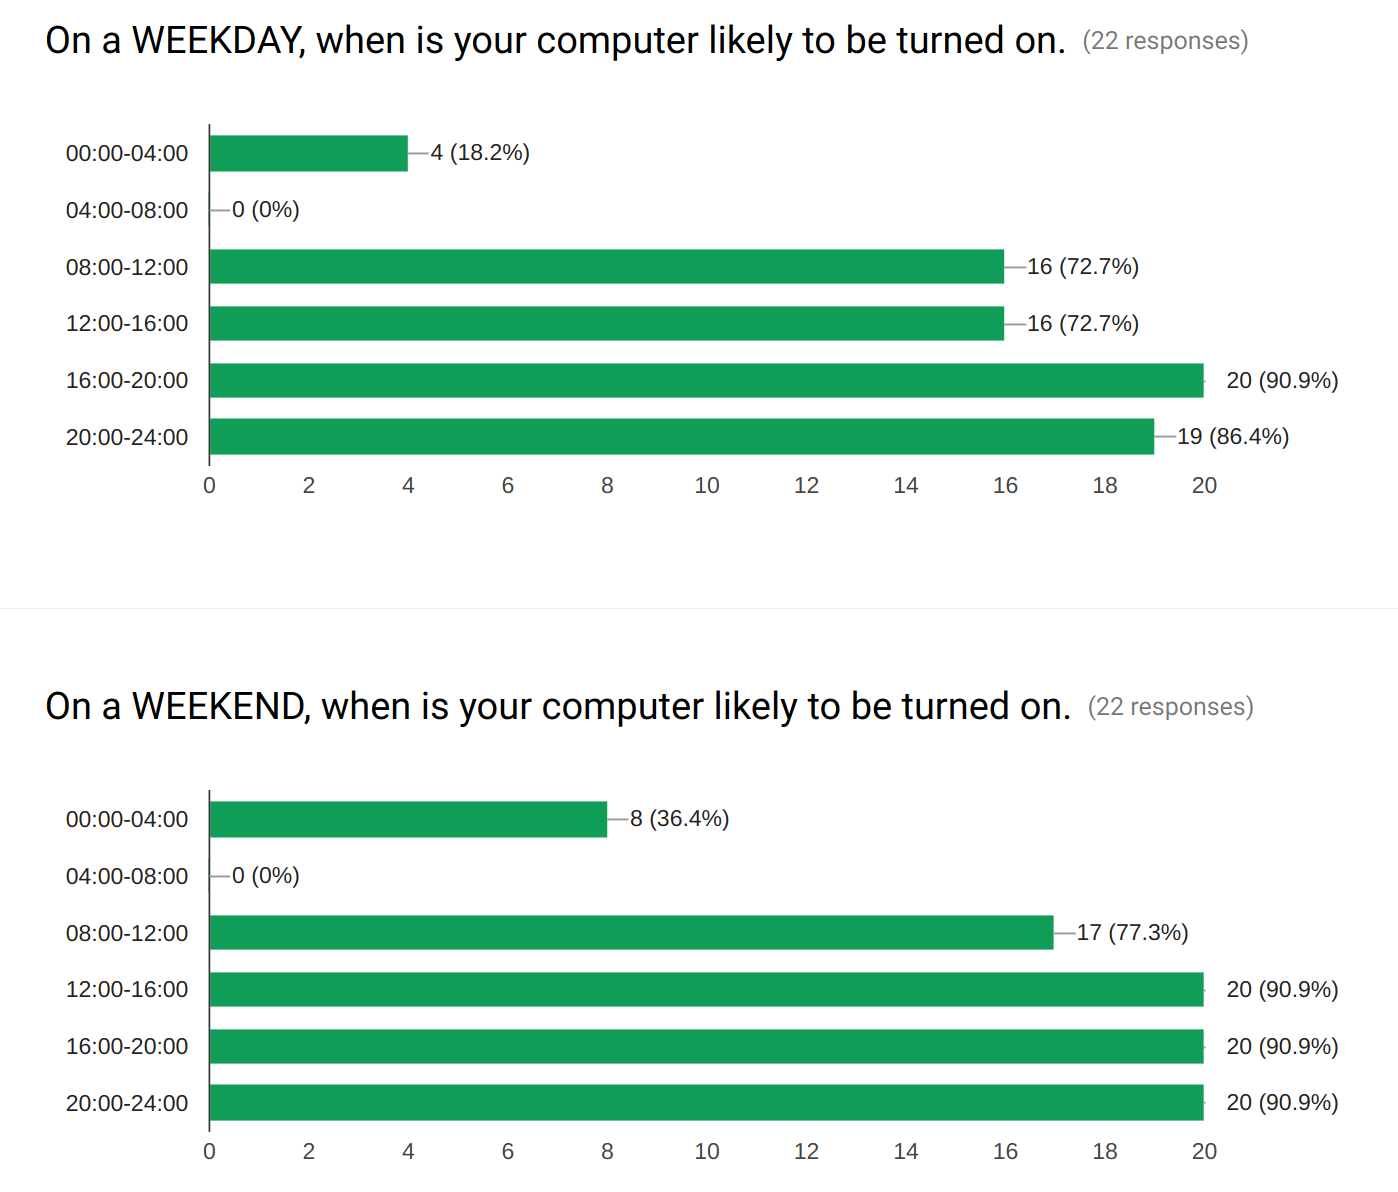
\includegraphics[width=\textwidth]{uptime-survey}
 \caption{Uptime Survey}
 \label{fig:uptime-survey}
\end{figure}

\pagebreak

\section{Images}

\begin{figure*}[!htb]
 \centering
 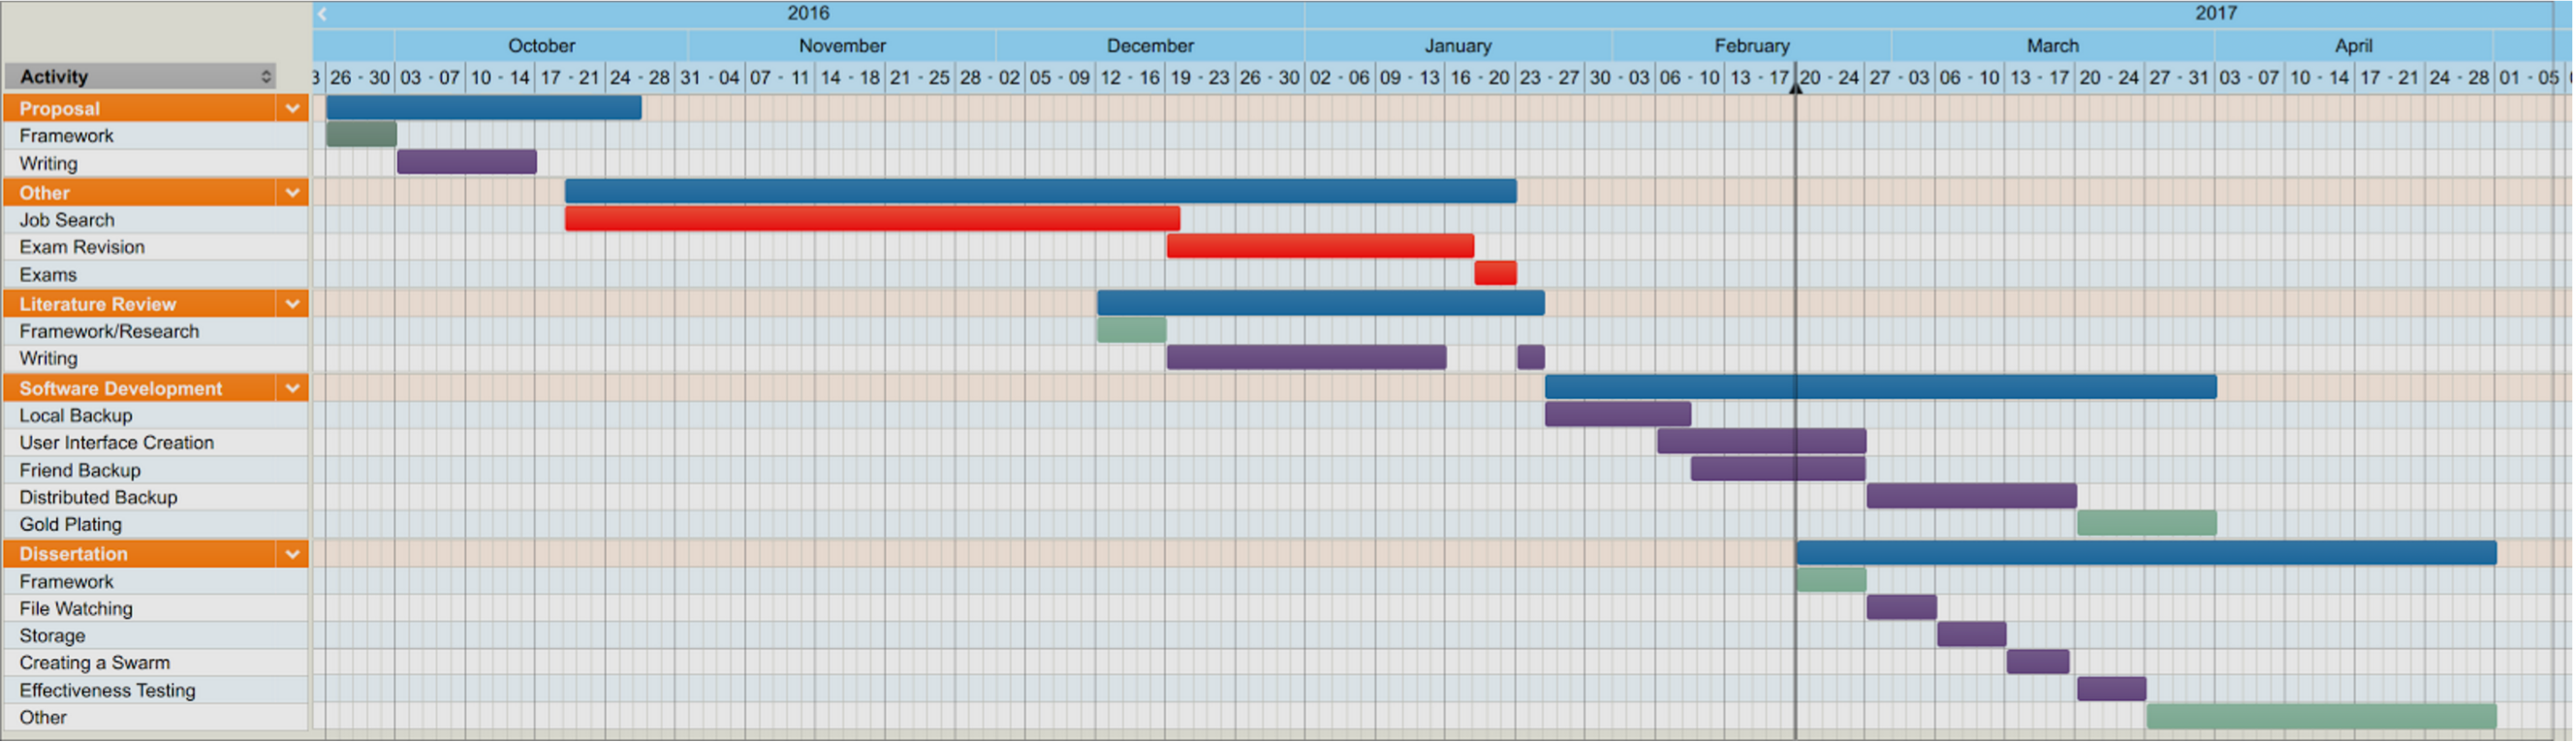
\includegraphics[width=\textwidth]{gantt}
 \caption{Gantt Chart (February 2017)}
 \label{fig:gantt}
\end{figure*}

\begin{figure*}[!htb]
 \centering
 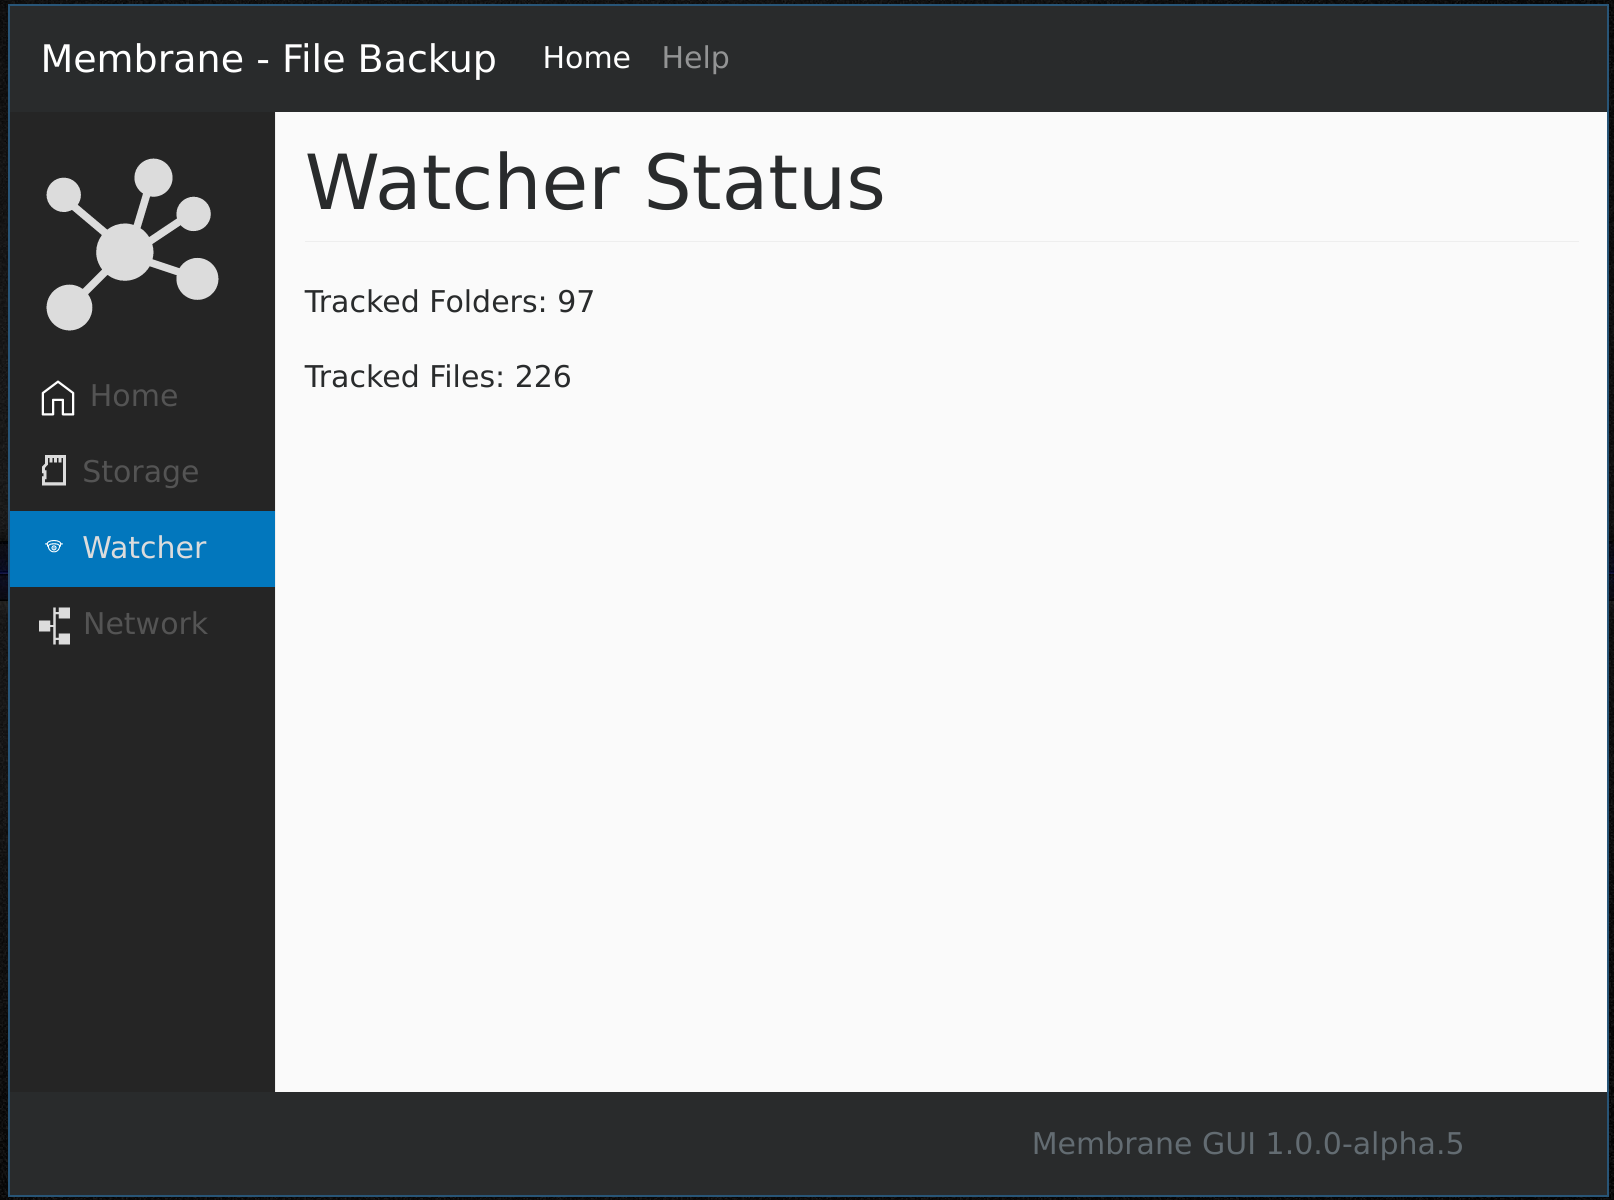
\includegraphics[width=\textwidth]{gui-watcher}
 \caption{GUI Watcher Screen}
 \label{fig:gui-watcher}
\end{figure*}

\begin{figure*}[!htb]
 \centering
 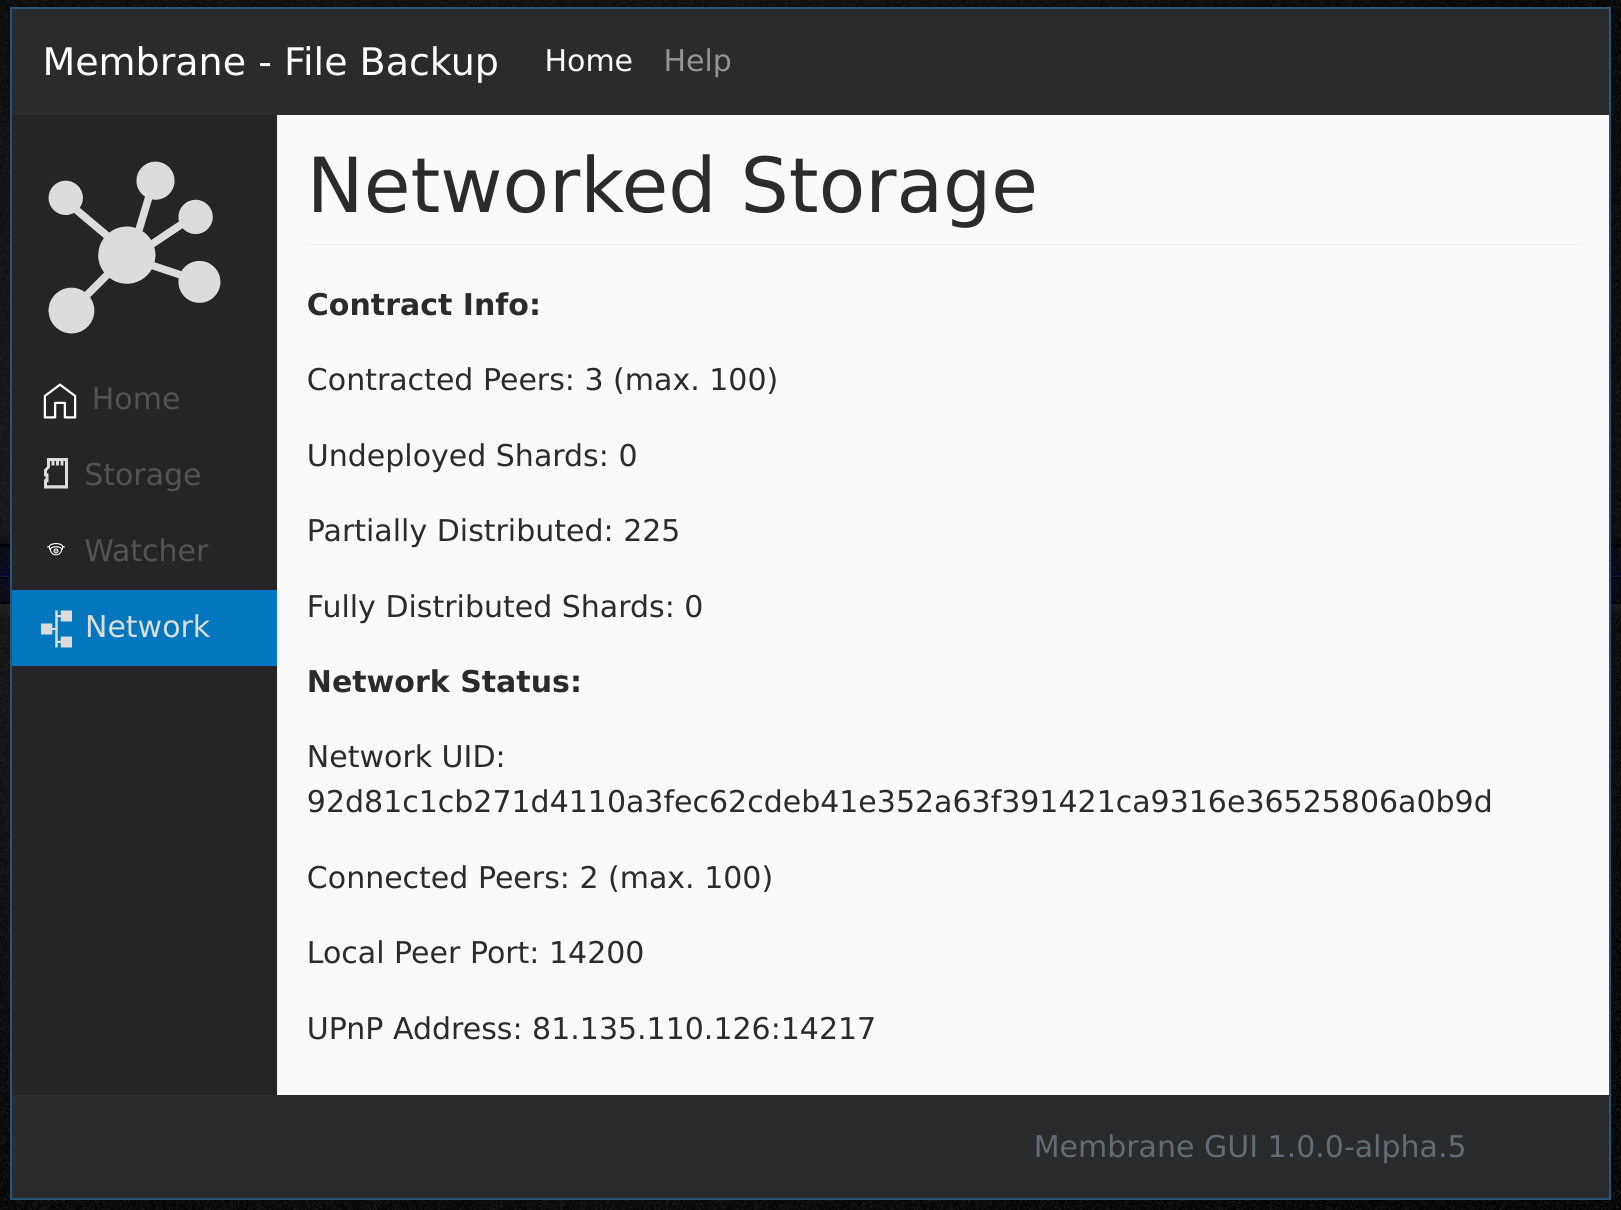
\includegraphics[width=\textwidth]{gui-network}
 \caption{GUI Network Screen}
 \label{fig:gui-network}
\end{figure*}

\begin{figure*}[!htb]
 \centering
 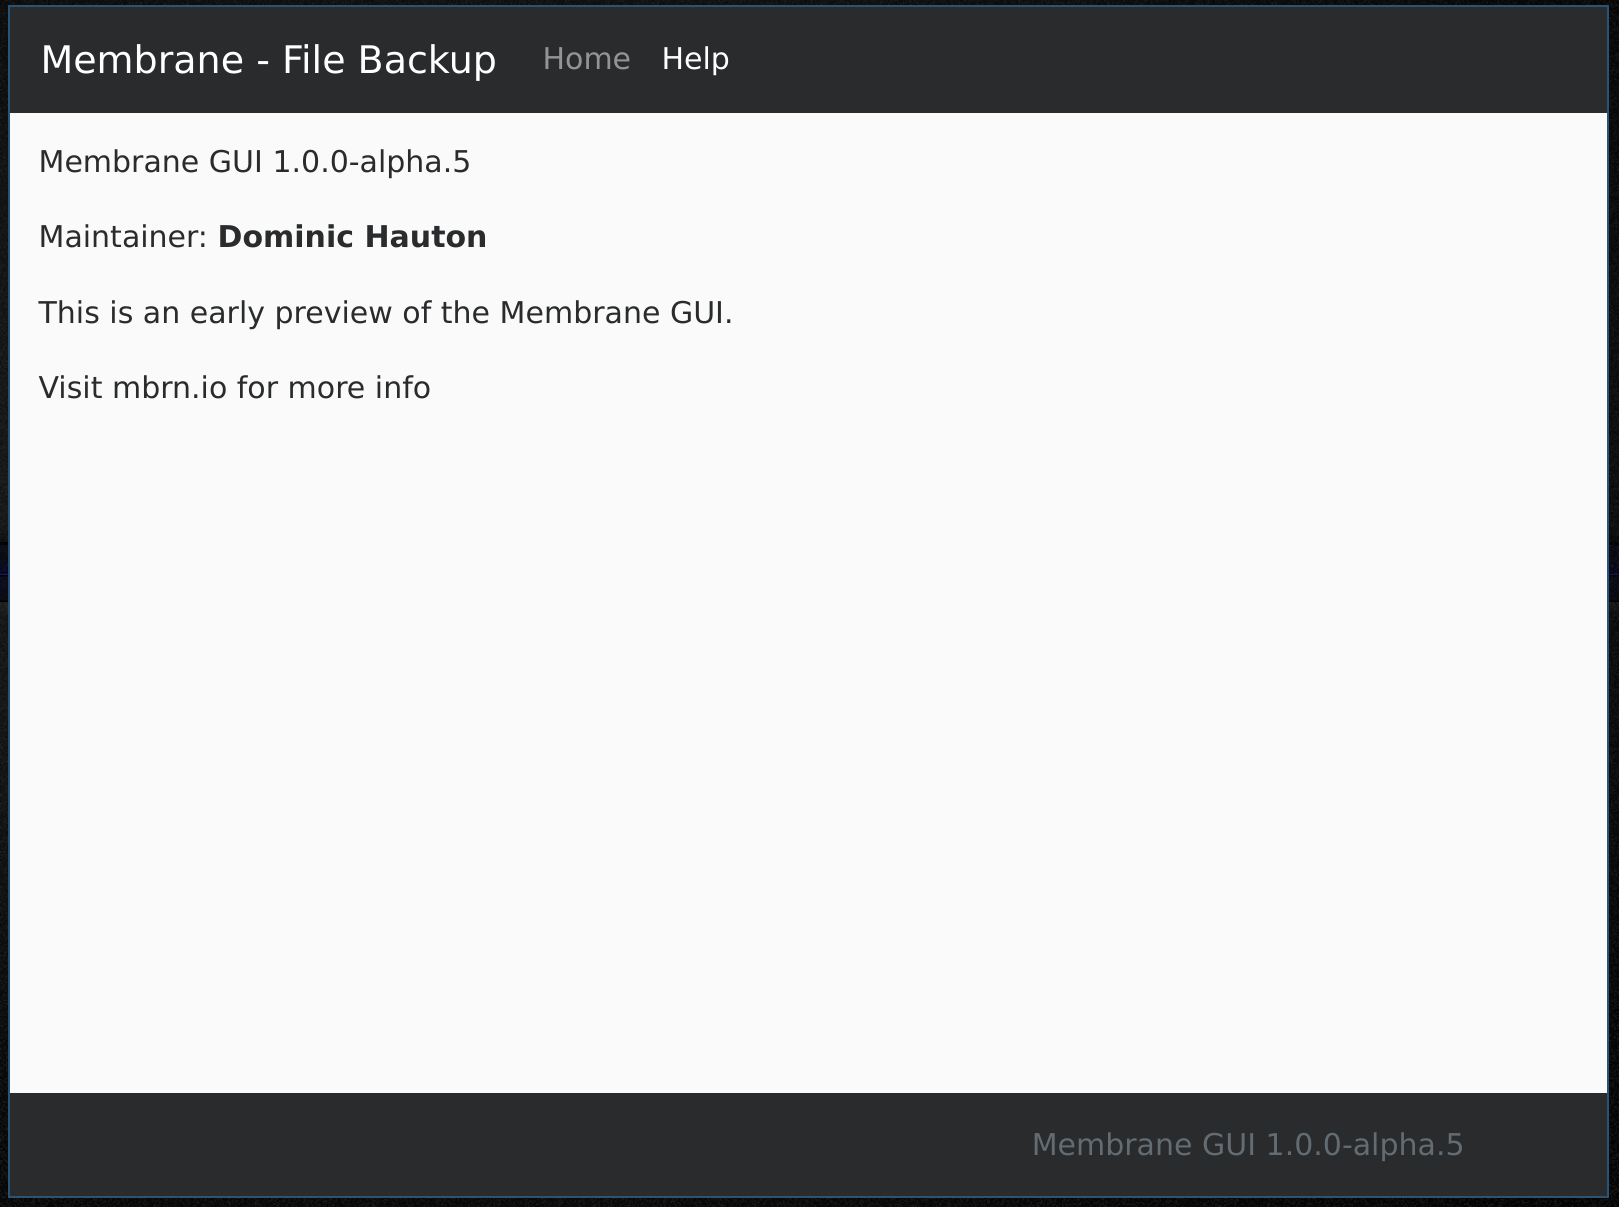
\includegraphics[width=\textwidth]{gui-help}
 \caption{GUI Help Screen}
 \label{fig:gui-help}
\end{figure*}

\end{document}
